\chapter{Evaluation}\label{chap:evaluation}
In this chapter, we present our evaluation criteria and the findings which we got from them.
We evaluate the four models with a three-pronged strategy, targeting the following characteristics:

\begin{enumerate}
    \item\textbf{Accuracy} - the share of correct next-activity predictions
    \item\textbf{Training time} - the amount of time required for training
    \item\textbf{Stability} - the change in prediction accuracy with progress
\end{enumerate}

The first two criteria target the general usability of each model.
We measure accuracy because it is a good indicator of how often the model predicts the right class, and permits comparisons to other works.
Different from typical machine learning evaluations, we do not measure recall, because it is not typically measured by works in Predictive Process Monitoring.
Training time is of interest because a real-world application should use as little computing ressources as possible.
The stability criterion permits making a judgment about the stability of the predictions. The works of Francescomarino et al.~\cite{francescomarino2015} and Klinkmüller et al.~\cite{klinkmuller2018reliablemonitoring}, inspired this measure. It provides an understanding of how the prediction accuracy of a model changes as the traces gets longer. This can facilitate building trust in the model, as indicated in the introduction of the thesis~\cite{klinkmuller2018reliablemonitoring, boehmer2018probability}.
During the evaluation, results for BPIC logs and the HelpDesk dataset should not be compared too closely, as the BPIC logs are a lot more resouceful in terms of data attributes.

We discuss the acurracy of the models in \autoref{sec:eval:accuracy}, followed by the discussion of the required training time in \autoref{sec:eval:training-time}. We go on to discuss stability in \autoref{sec:eval:stability}, and conclude the chapter in \autoref{sec:eval:discussion}.

\section{Accuracy}\label{sec:eval:accuracy}
The accuracy on unseen data is a good indicator of the prediction performance of any prediction model.
It is the share of correct predictions that match their target labels, among the number of total predictions:

$$\frac{n_{correct}}{n_{total}} $$

In the following paragraphs, we present the maximum accuracies obtained on the validation set of each log.
For each log, we show a plot of the different model accuracies, grouped by batching strategy.
The presentation of the logs is ordered by process complexity, similar to \autoref{tab:dataset-characteristics}.
We end the section with a verdict of the observations.\\

% individual strategy
\paragraph{Accuracy on HelpDesk}
\autoref{fig:max-accuracies-helpdesk} displays the different accuracies on the validation set from HelpDesk log.
With the individual, grouping and padding strategies, the SCH, SP2 and PFS models score above $0.80$.
As expected, the windowing strategy impacts accuracy significantly, with all models seeing large degradations in accuracy.
The SP2 model is impacted the least by the windowing strategy, presumably because its SP2 features capture the history that is cut away.
While the SCH, SP2 and PFS models do not show strong reactions to changes in the first three batching strategies, the accuracies by the EVM model fluctuate immensely.
On the individual strategy, it exhibits $0.724$; $0.316$ and $0.3$ on the grouping and padding strategies.

\begin{figure}[!htb]
    \centering
    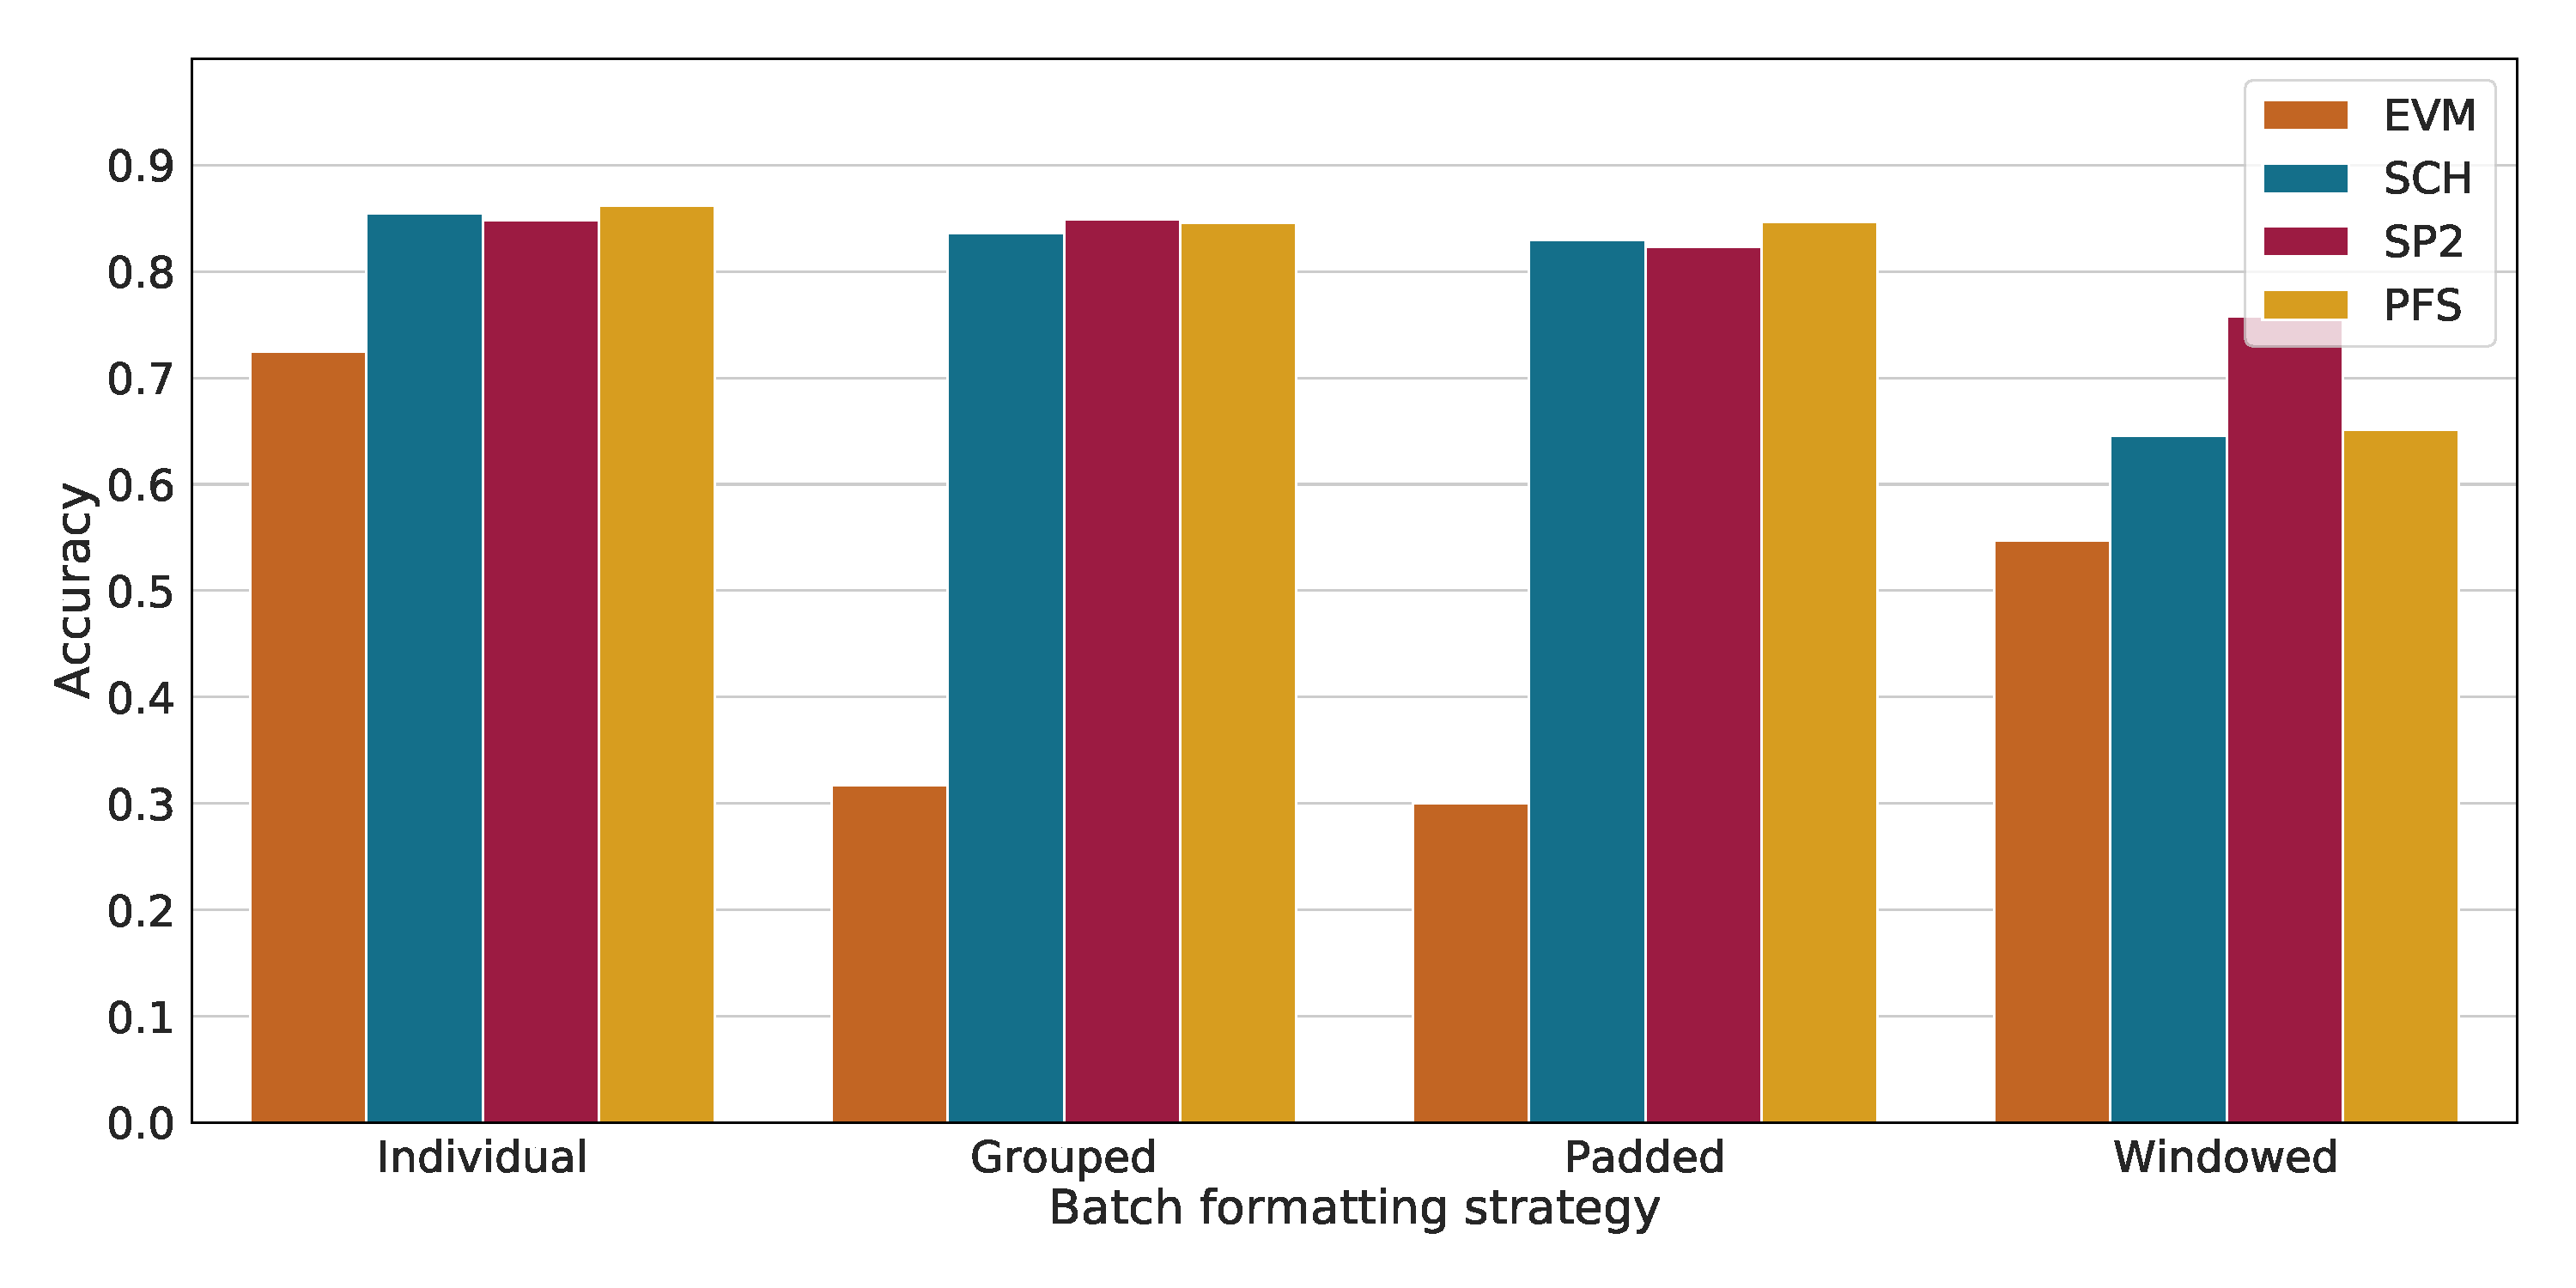
\includegraphics[width=\textwidth]{gfx/helpdesk/accuracies.pdf}
    \caption{Best accuracies on the validation set of HelpDesk}
    \label{fig:max-accuracies-helpdesk}
\end{figure}

\paragraph{Accuracy on BPIC12}
BPIC12 is small step up in process complexity, and the accuracy measurements are visualized in \autoref{fig:max-accuracies-bpic2012}.
Again, the EVM, SCH, and SP2 models exhibit very similar accuracies for the three batching strategies that supply the complete process history.
With the individual and padding strategies, all three of them reach over $0.840$.
In the case of the grouping strategy, the tree accuracies are between $0.750$ and $0.765$.h
We attribute the small drop in accuracy with the grouping strategy to the large batch sizes that the strategy produces (cf. \autoref{tab:dataset-characteristics}).
The windowing strategy leads to bigger differences between the three SCH, SP2 and PFS models.
The SP2 model performs the best here as well, presumably because of its features.
The worst performance is again shown by the EVM model on all four strategies.
Its accuracies with the individual and grouping strategies are very similar.

\begin{figure}[!htb]
    \centering
    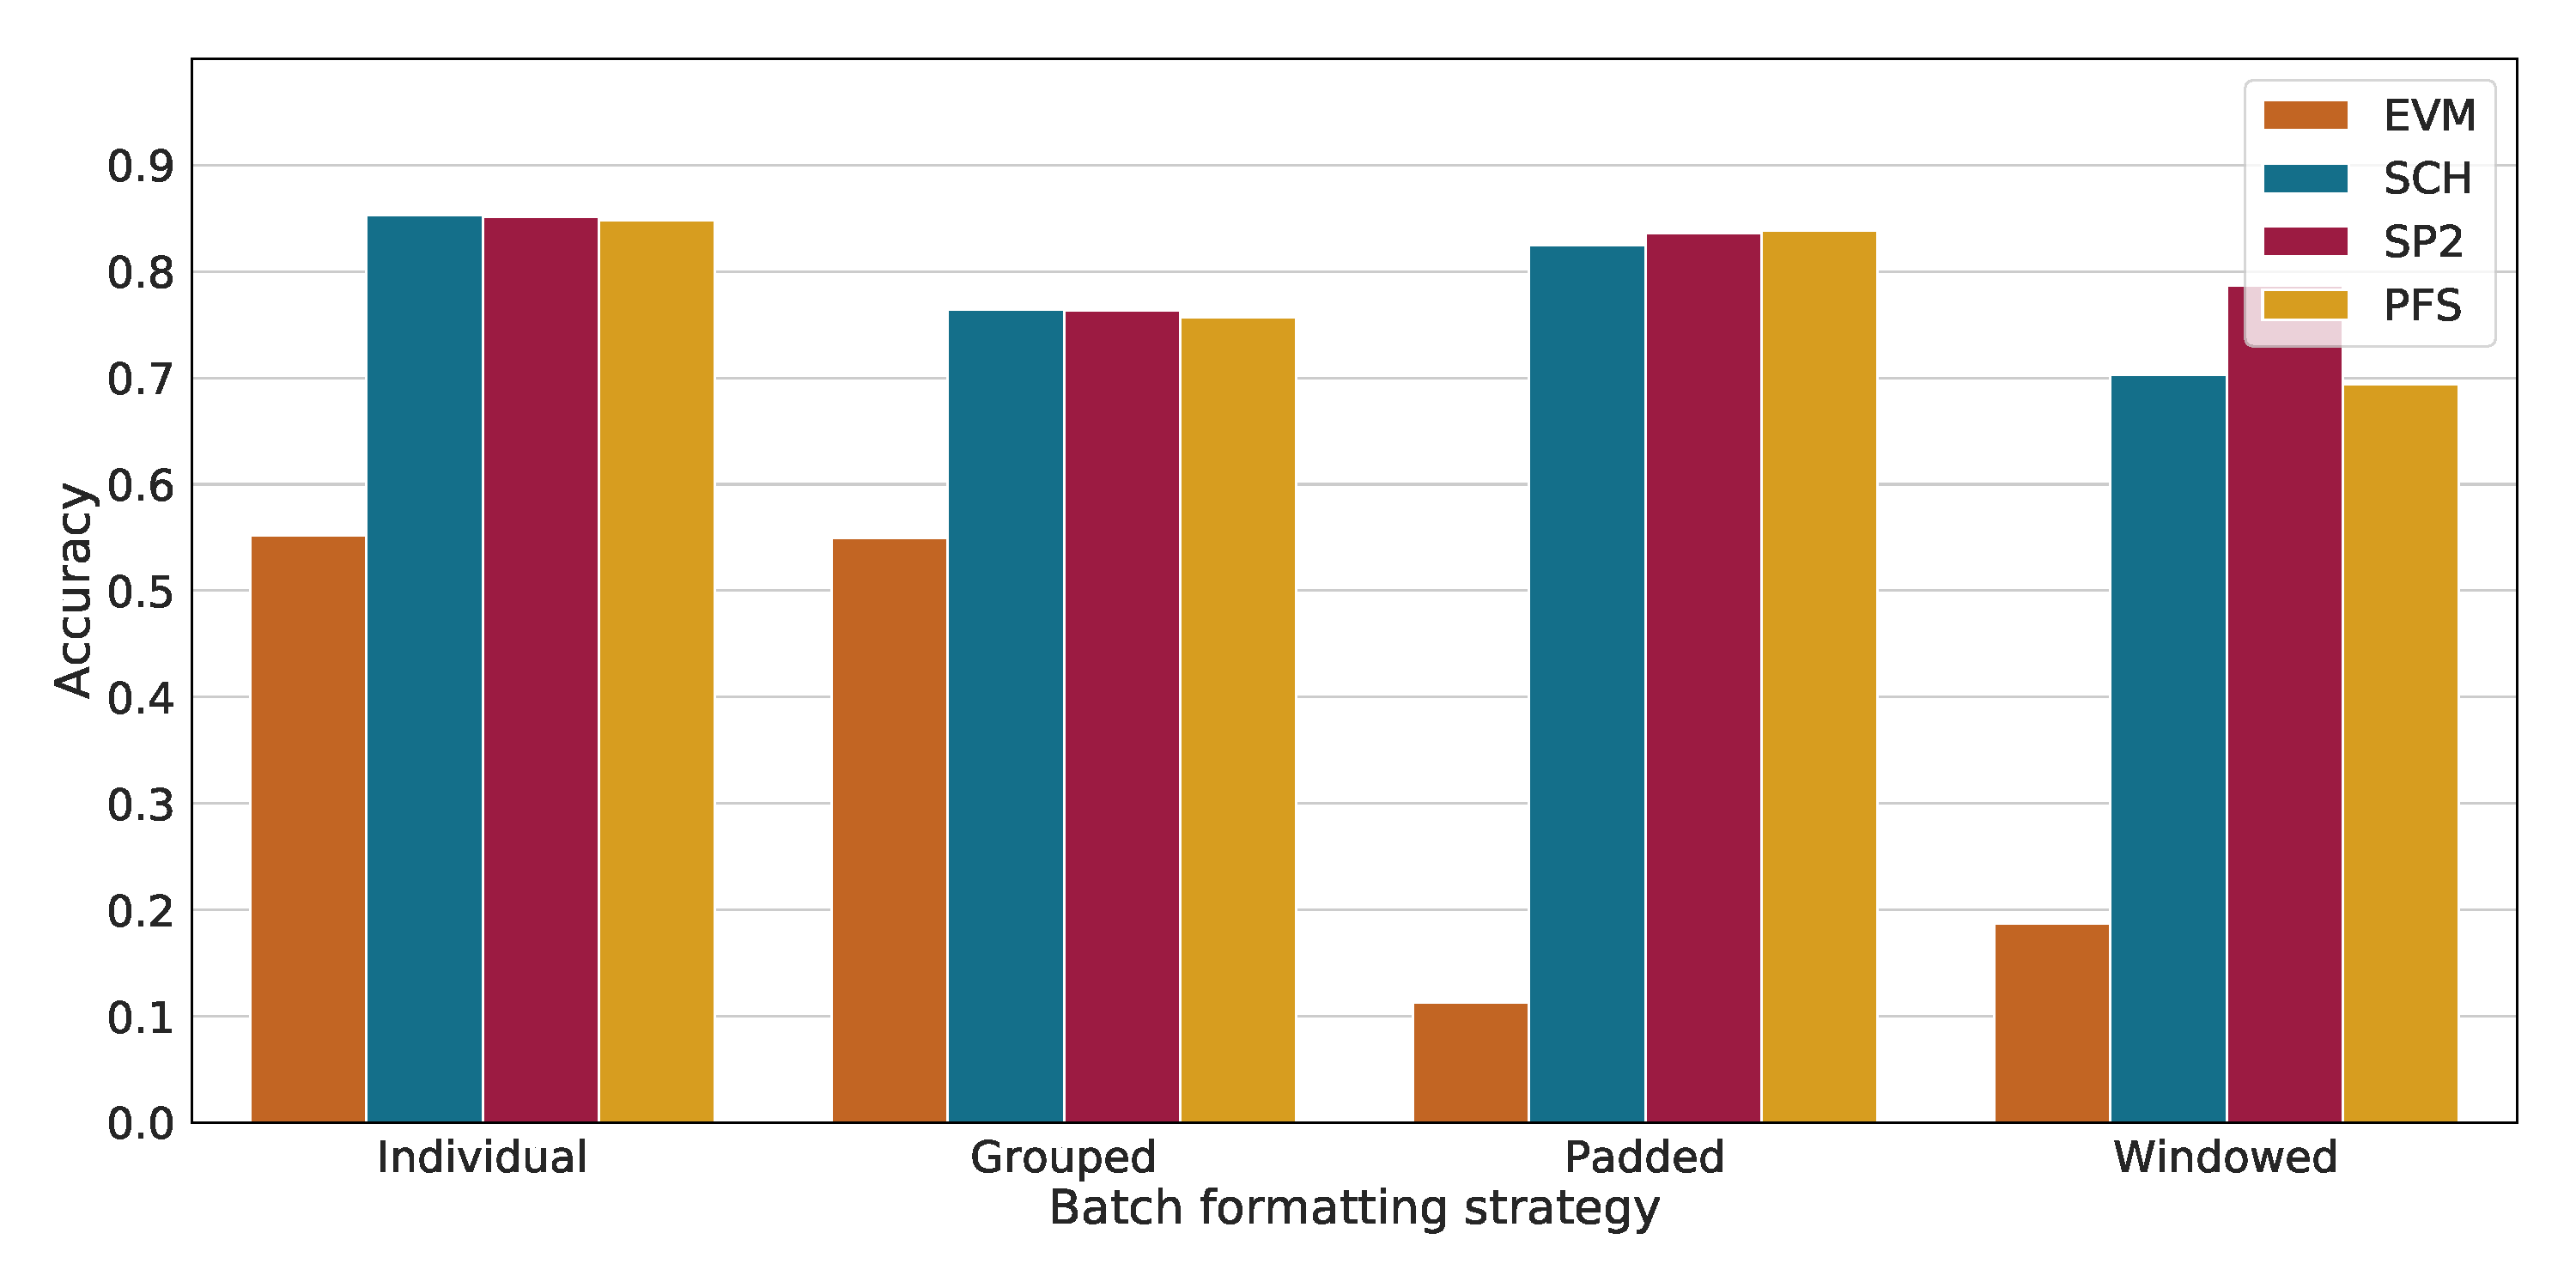
\includegraphics[width=\textwidth]{gfx/bpic2012/accuracies.pdf}
    \caption{Best accuracies on the validation set of BPIC12}
    \label{fig:max-accuracies-bpic2012}
\end{figure}

\paragraph{Accuracy on BPIC15}
The accuracies obtained on the validation sets of the BPIC15 logs are visualized in \autoref{fig:max-accuracies-bpic2015-1} to \autoref{fig:max-accuracies-bpic2015-5}.
Four common themes emerge in the plots:

First, the accuracies of the SCH, SP2 and PFS models are very similar across the individual, grouping and padding strategies.

Second, the SCH model always gives the highest accuracy of the four models with the individual strategy.

Third, the SP2 model gives the highest accuracies on all other strategies.
Also, its accuracies on the windowing strategy are the highest by far.
We presume that this is caused by the SP-2 features which encode some of the history that was cut away during windowing.

Fourth, the EVM model accuracies are unusable. While still above $0.1$ on the individual and grouping strategies, the model completely breaks down on the others.

\begin{figure}[!htb]
    \centering
    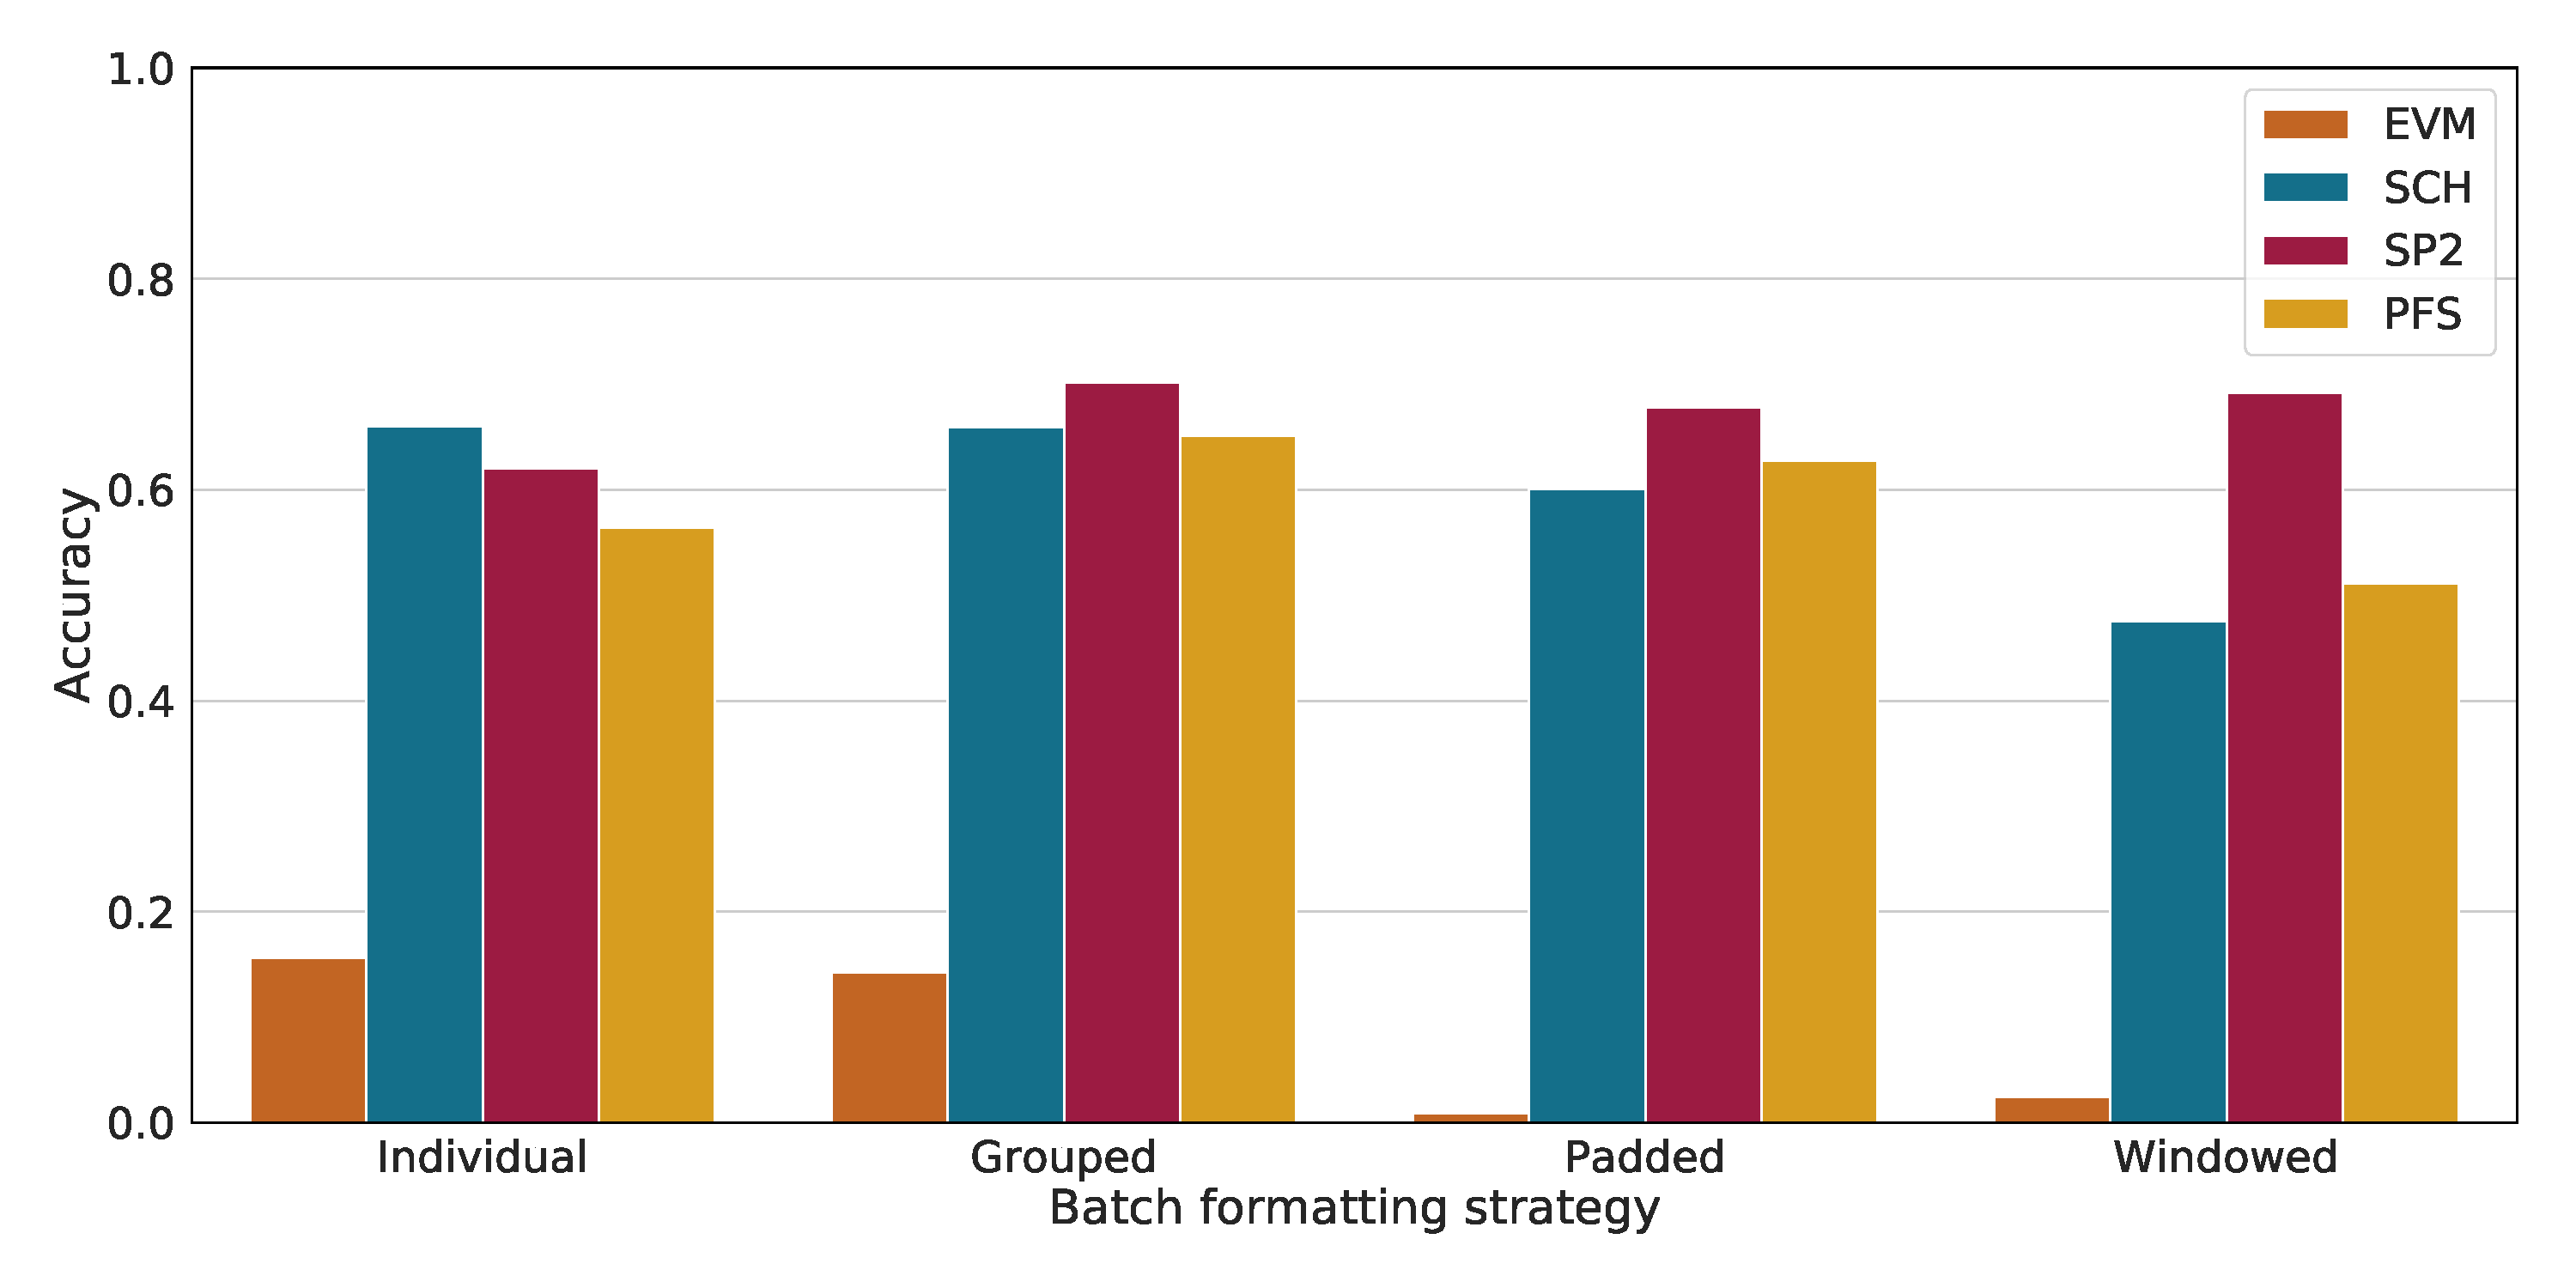
\includegraphics[width=\textwidth]{gfx/bpic2015_1/accuracies.pdf}
    \caption{Best accuracies on the validation set of BPIC15-1}
    \label{fig:max-accuracies-bpic2015-1}
\end{figure}
\begin{figure}[!htb]
    \centering
    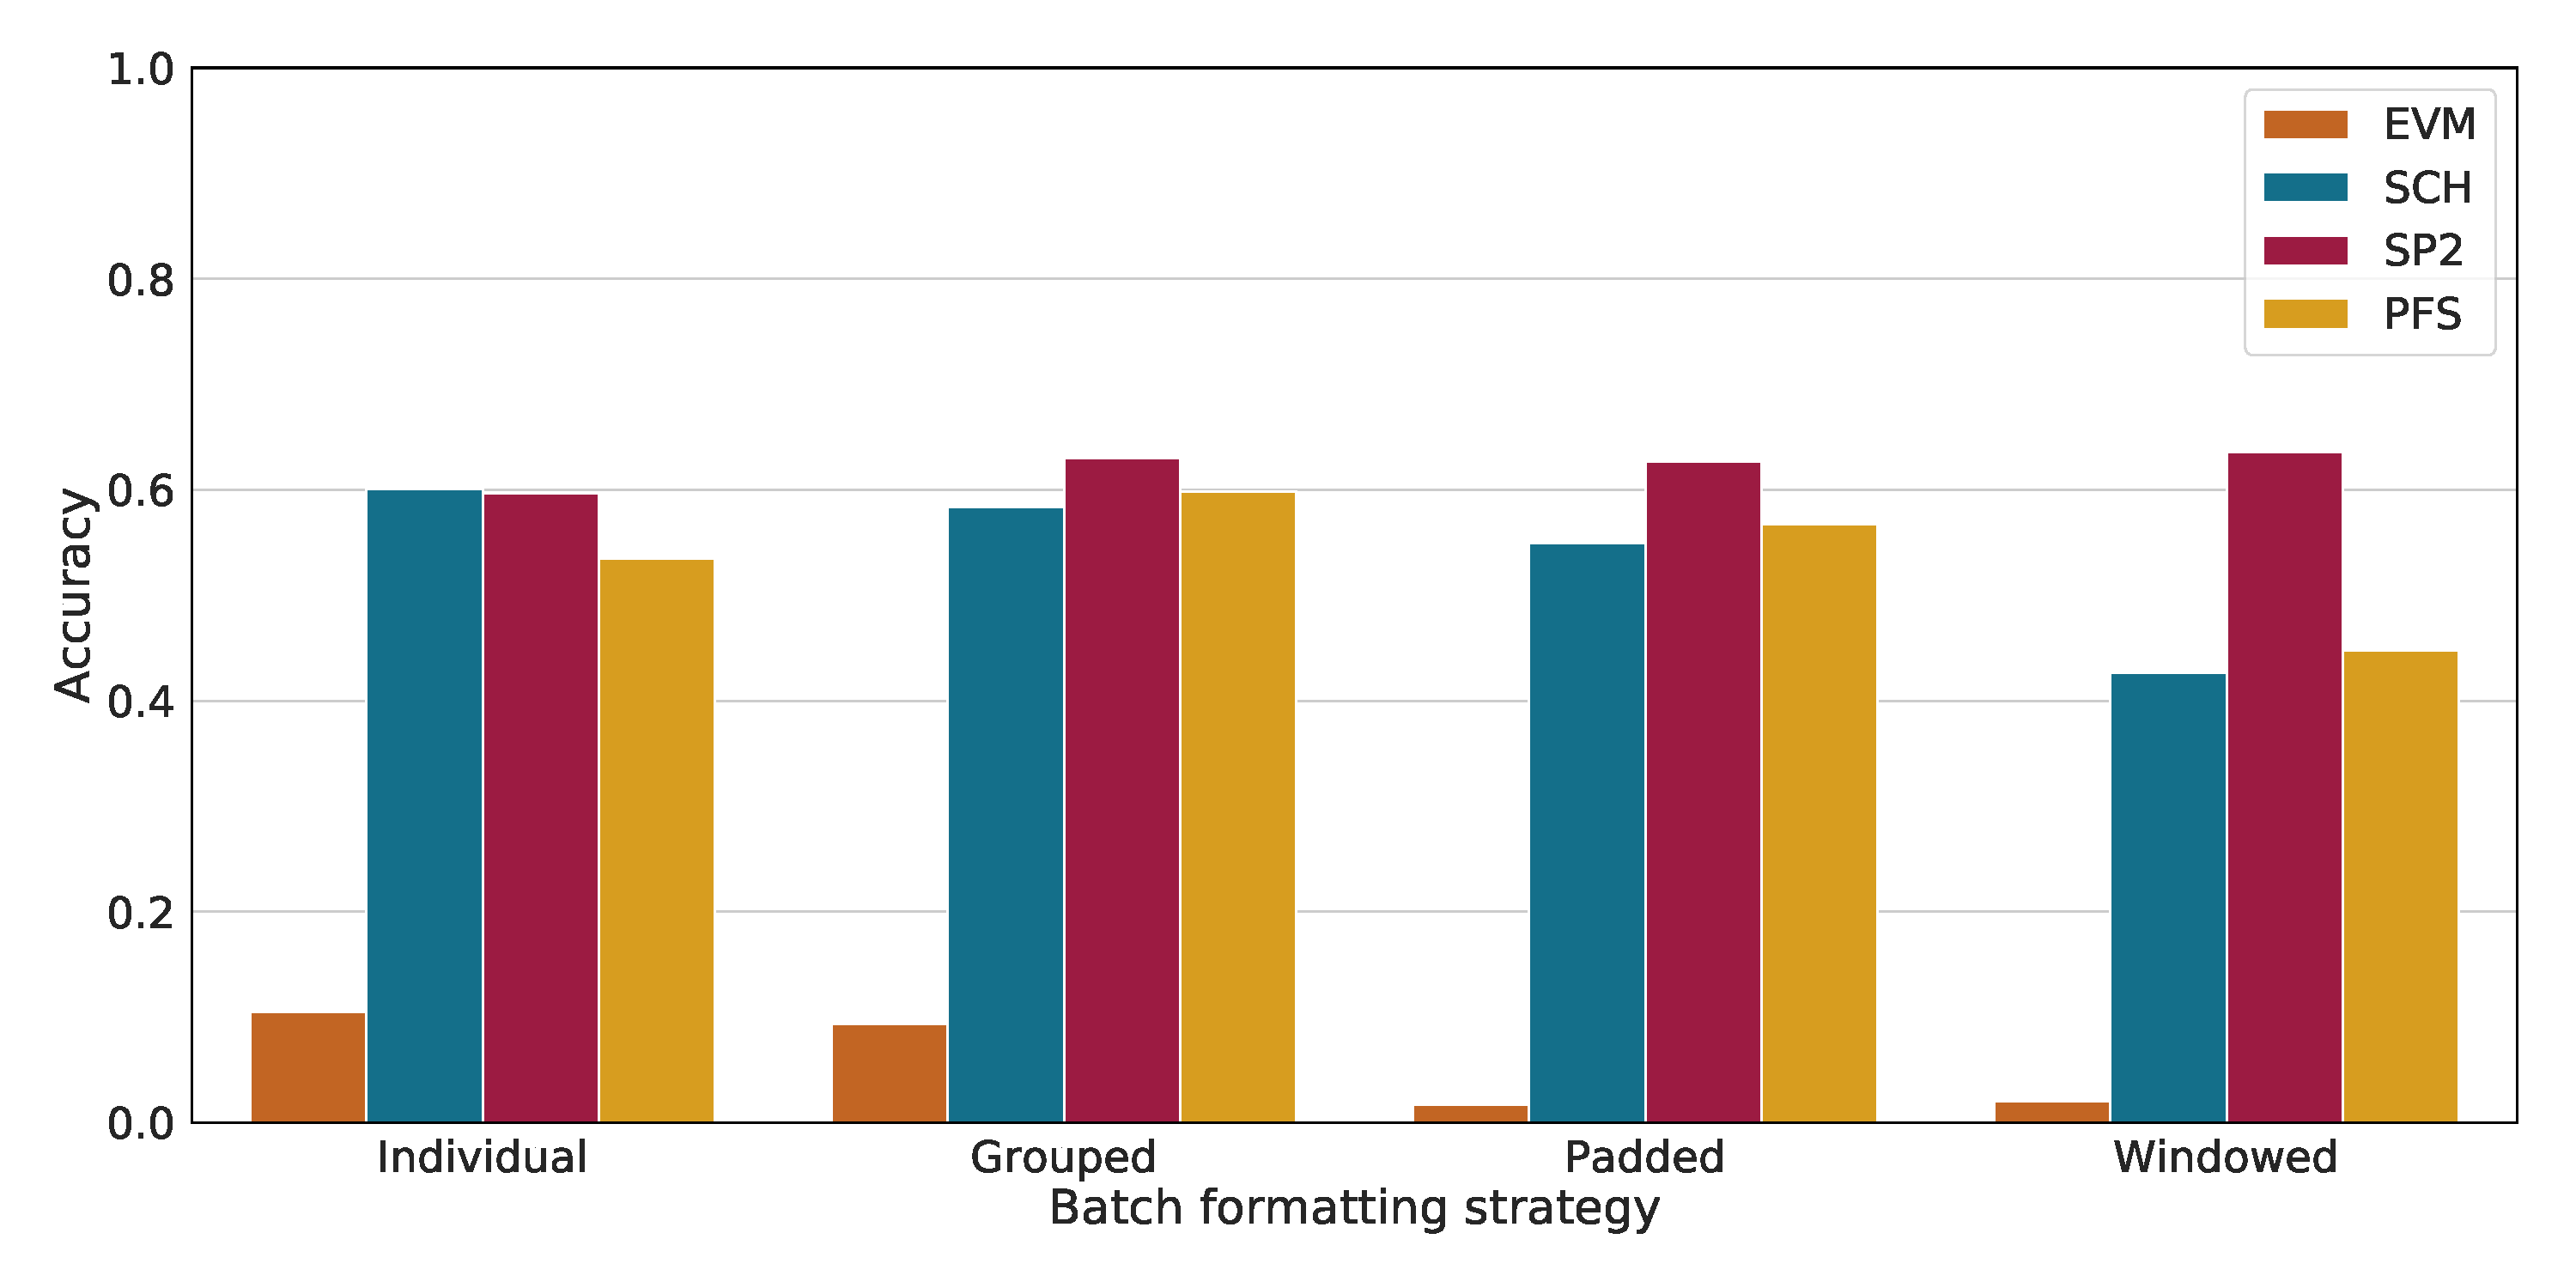
\includegraphics[width=\textwidth]{gfx/bpic2015_2/accuracies.pdf}
    \caption{Best accuracies on the validation set of BPIC15-2}
    \label{fig:max-accuracies-bpic2015-2}
\end{figure}
\begin{figure}[!htb]
    \centering
    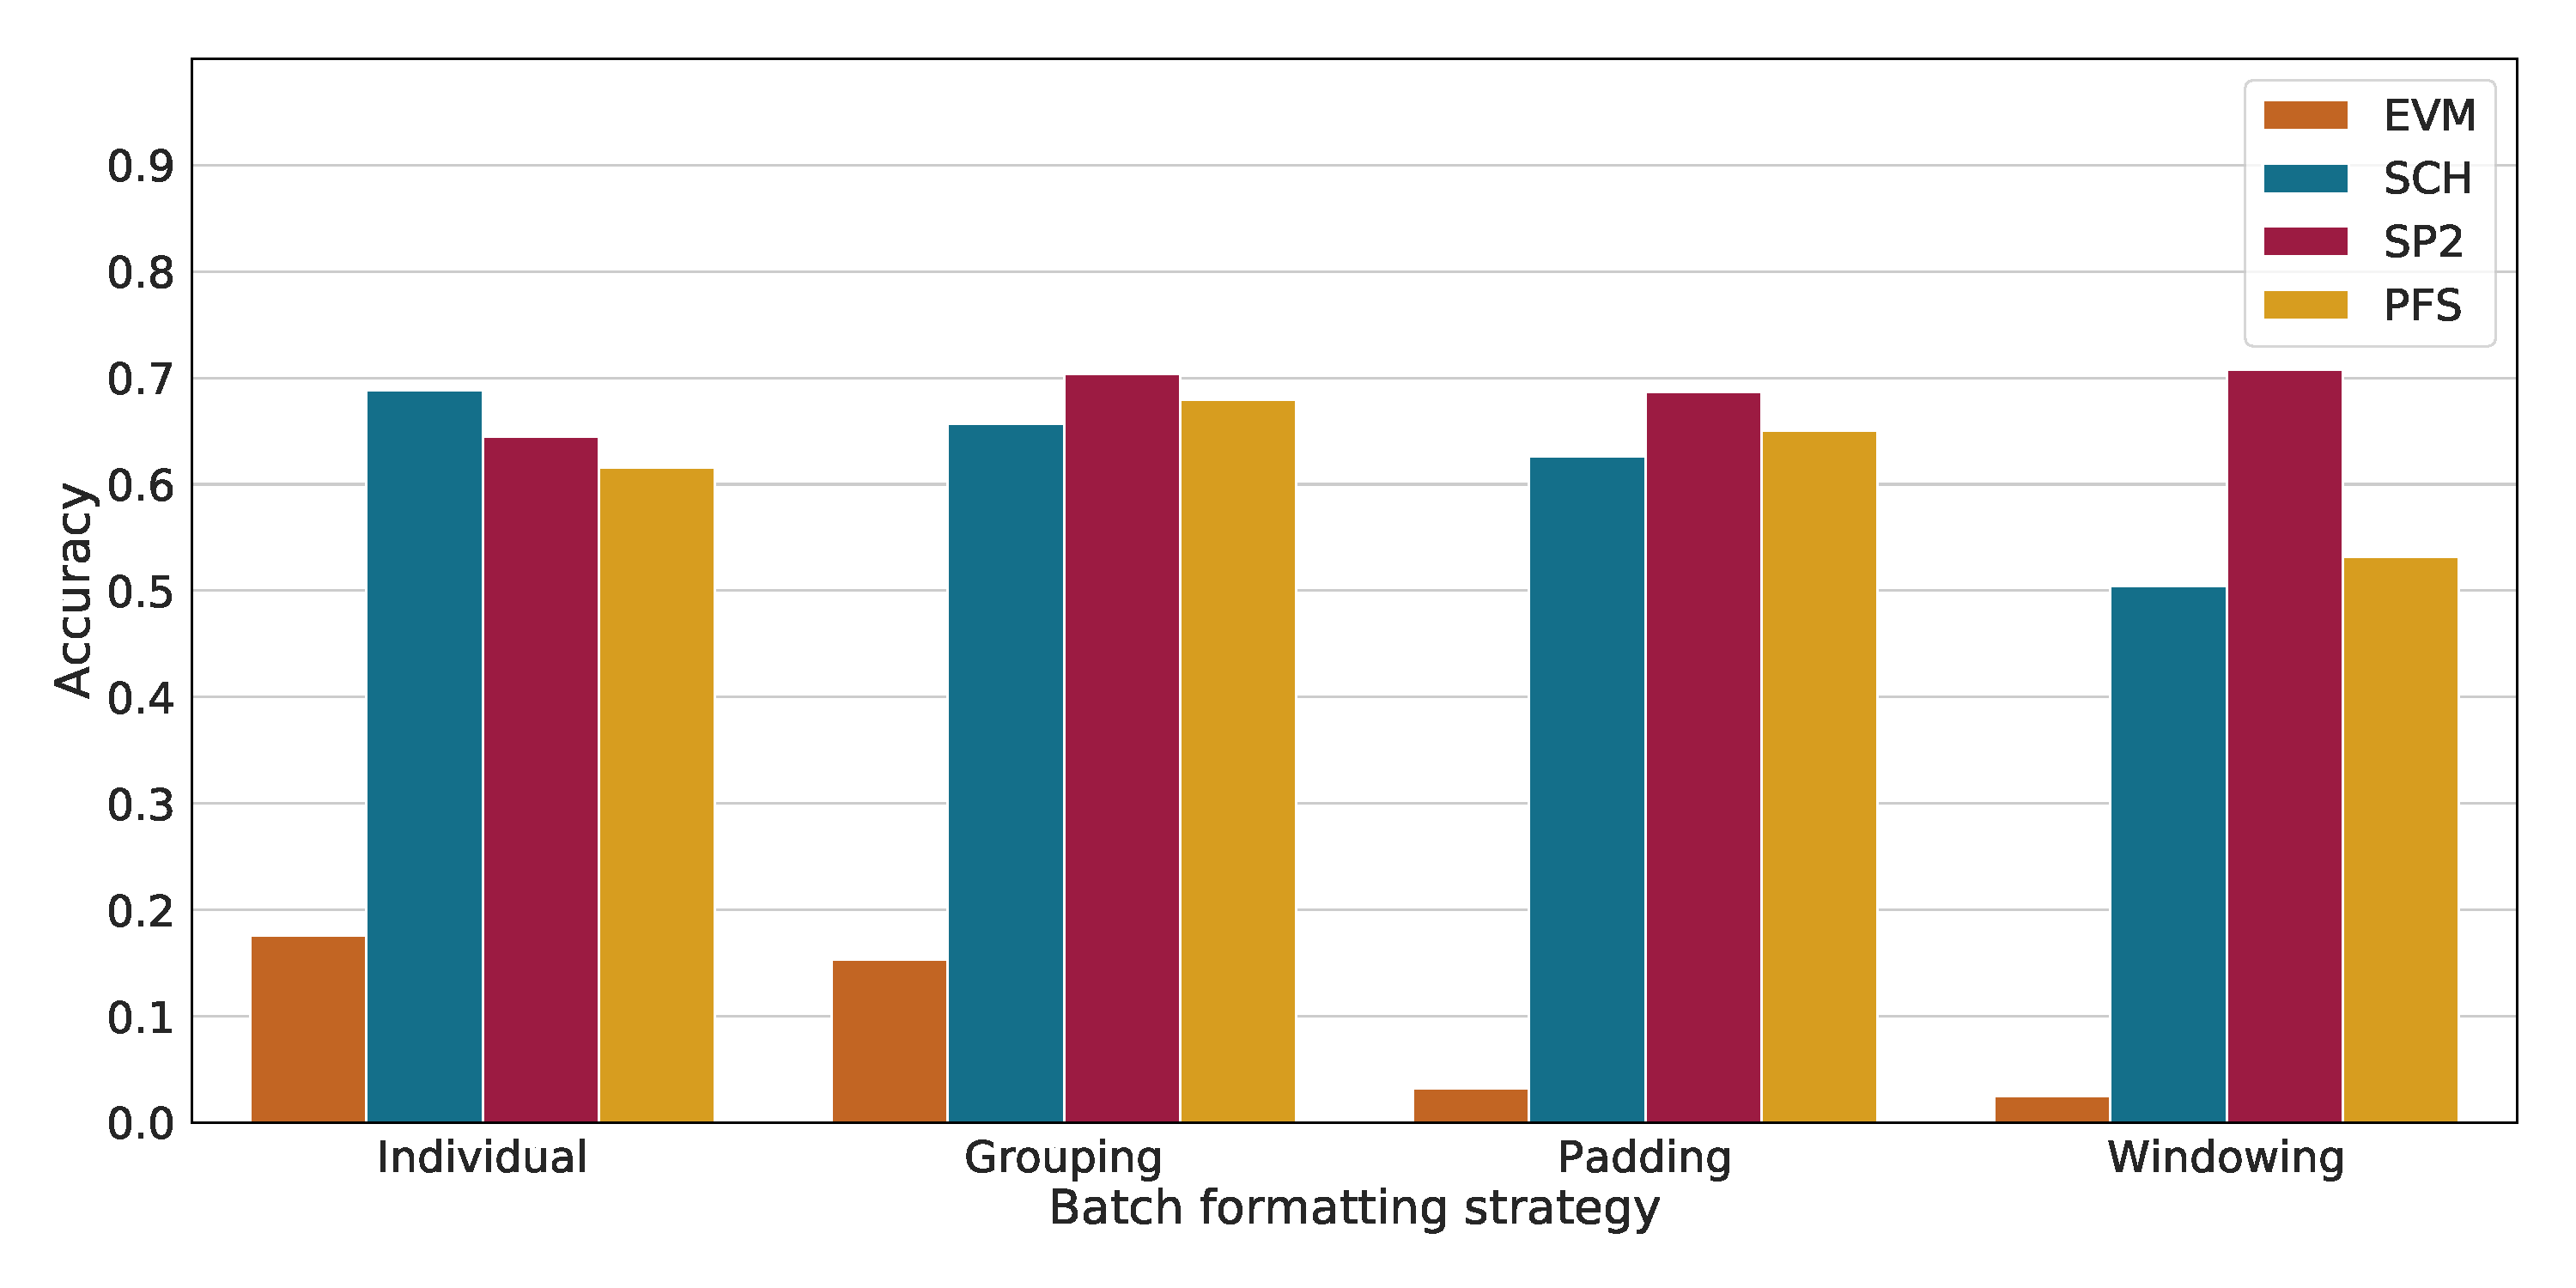
\includegraphics[width=\textwidth]{gfx/bpic2015_3/accuracies.pdf}
    \caption{Best accuracies on the validation set of BPIC15-3}
    \label{fig:max-accuracies-bpic2015-3}
\end{figure}
\begin{figure}[!htb]
    \centering
    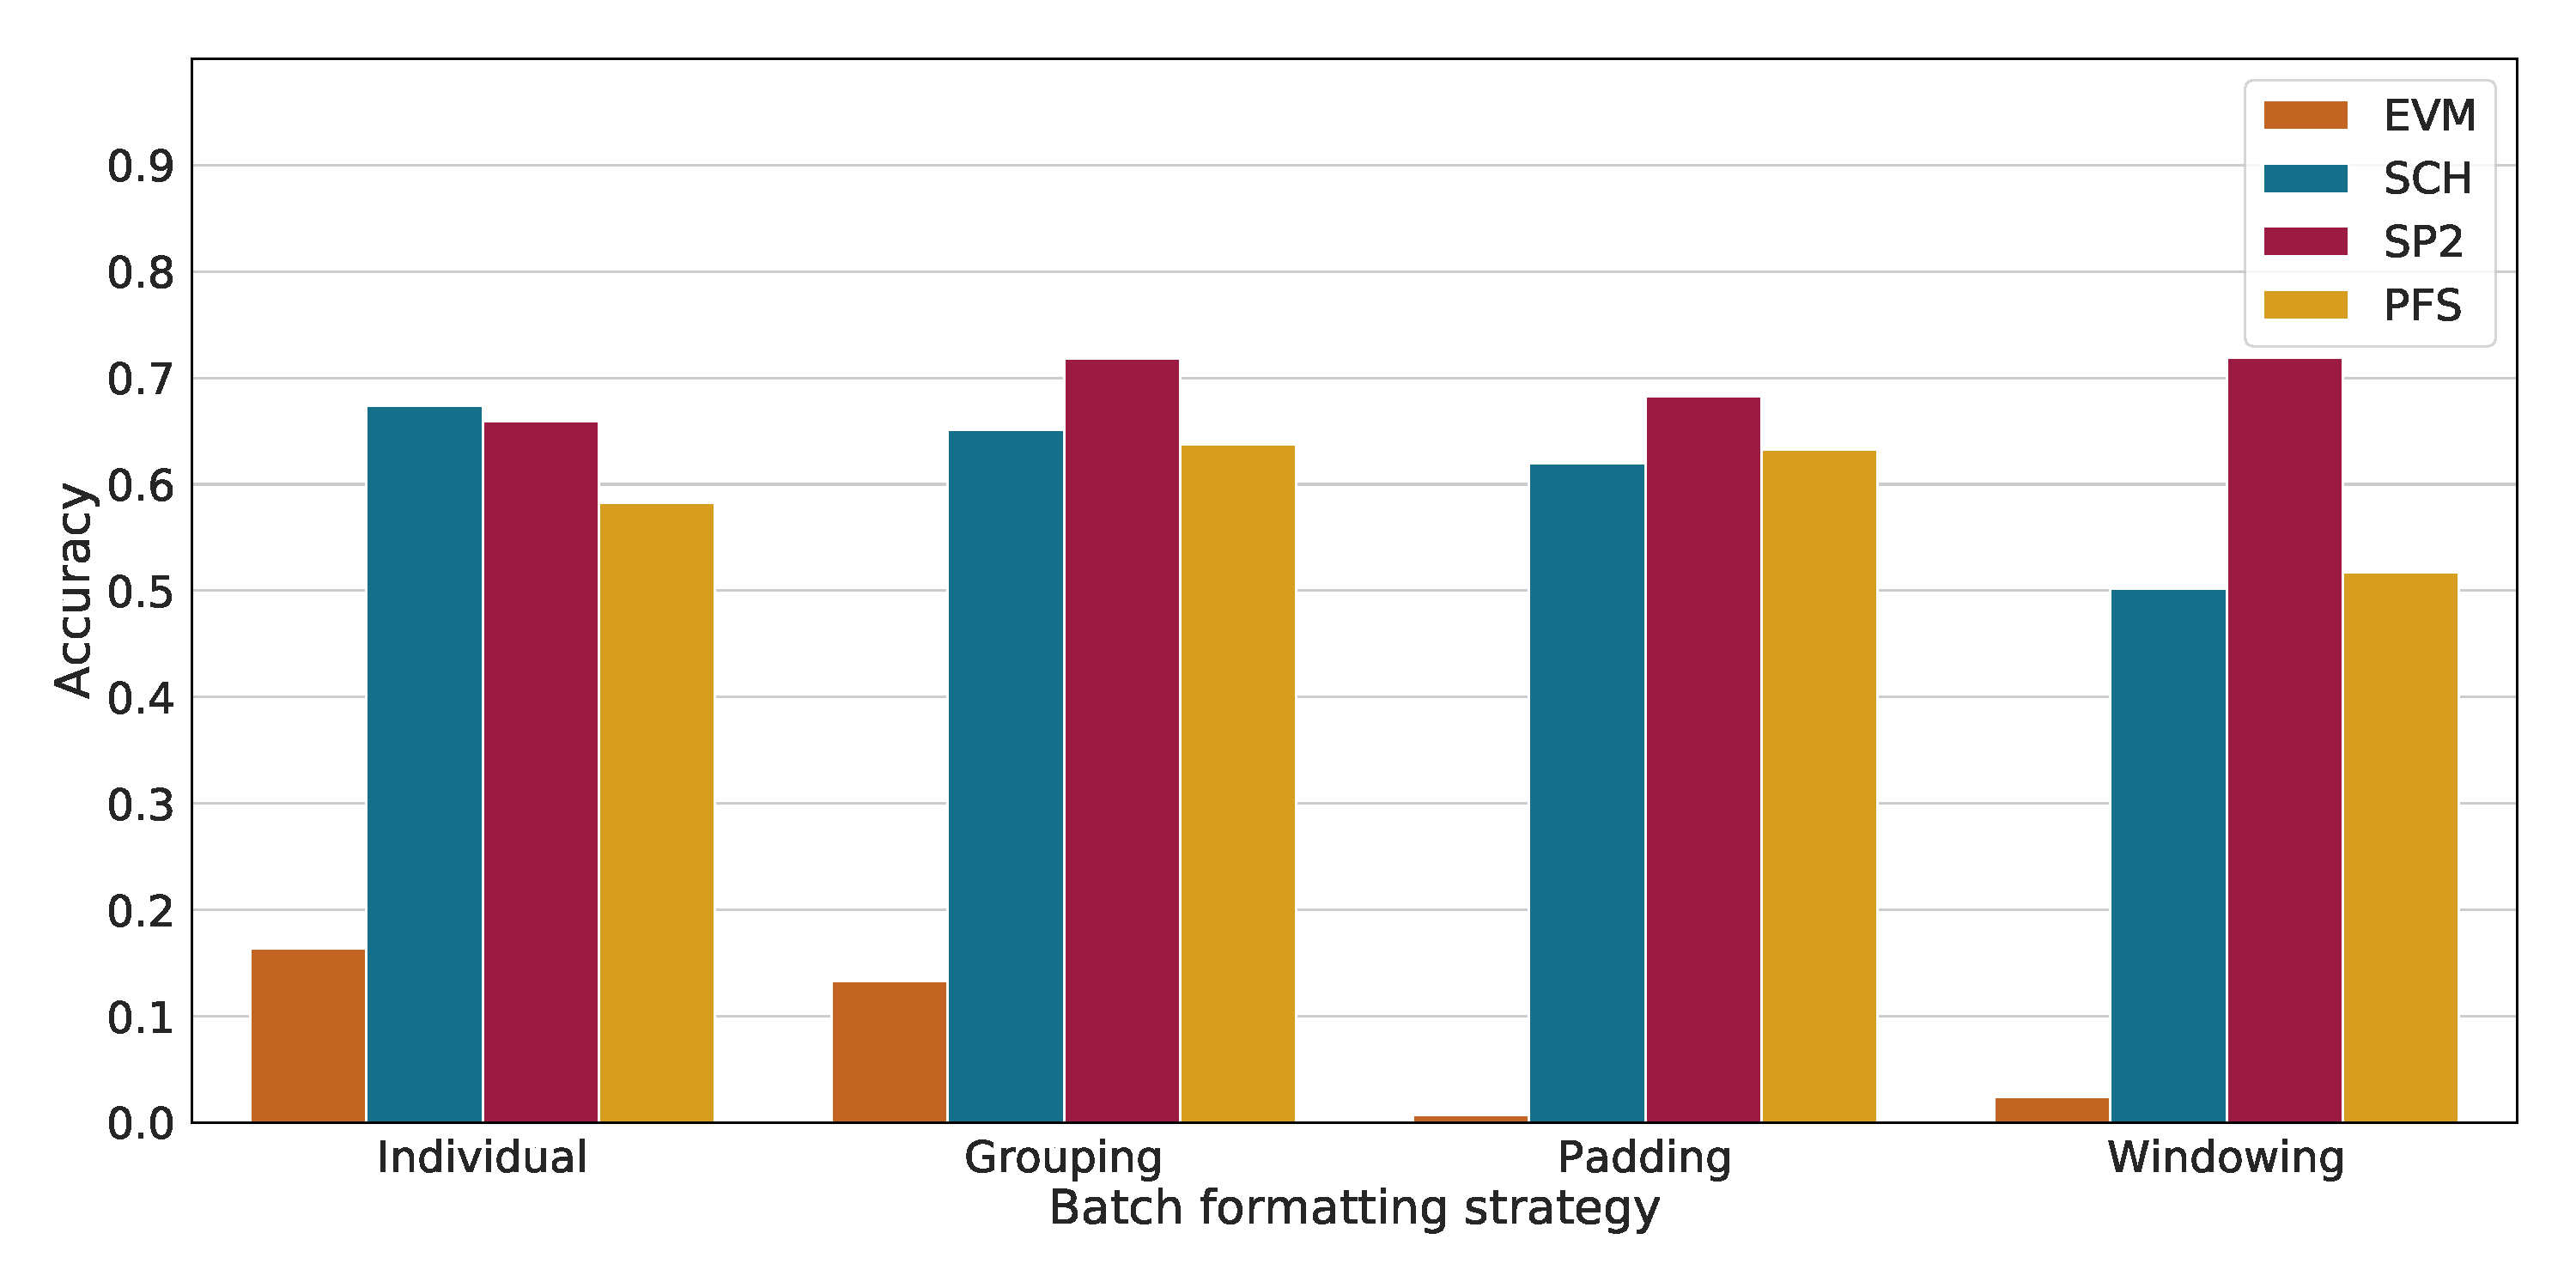
\includegraphics[width=\textwidth]{gfx/bpic2015_4/accuracies.pdf}
    \caption{Best accuracies on the validation set of BPIC15-4}
    \label{fig:max-accuracies-bpic2015-4}
\end{figure}
\begin{figure}[!htb]
    \centering
    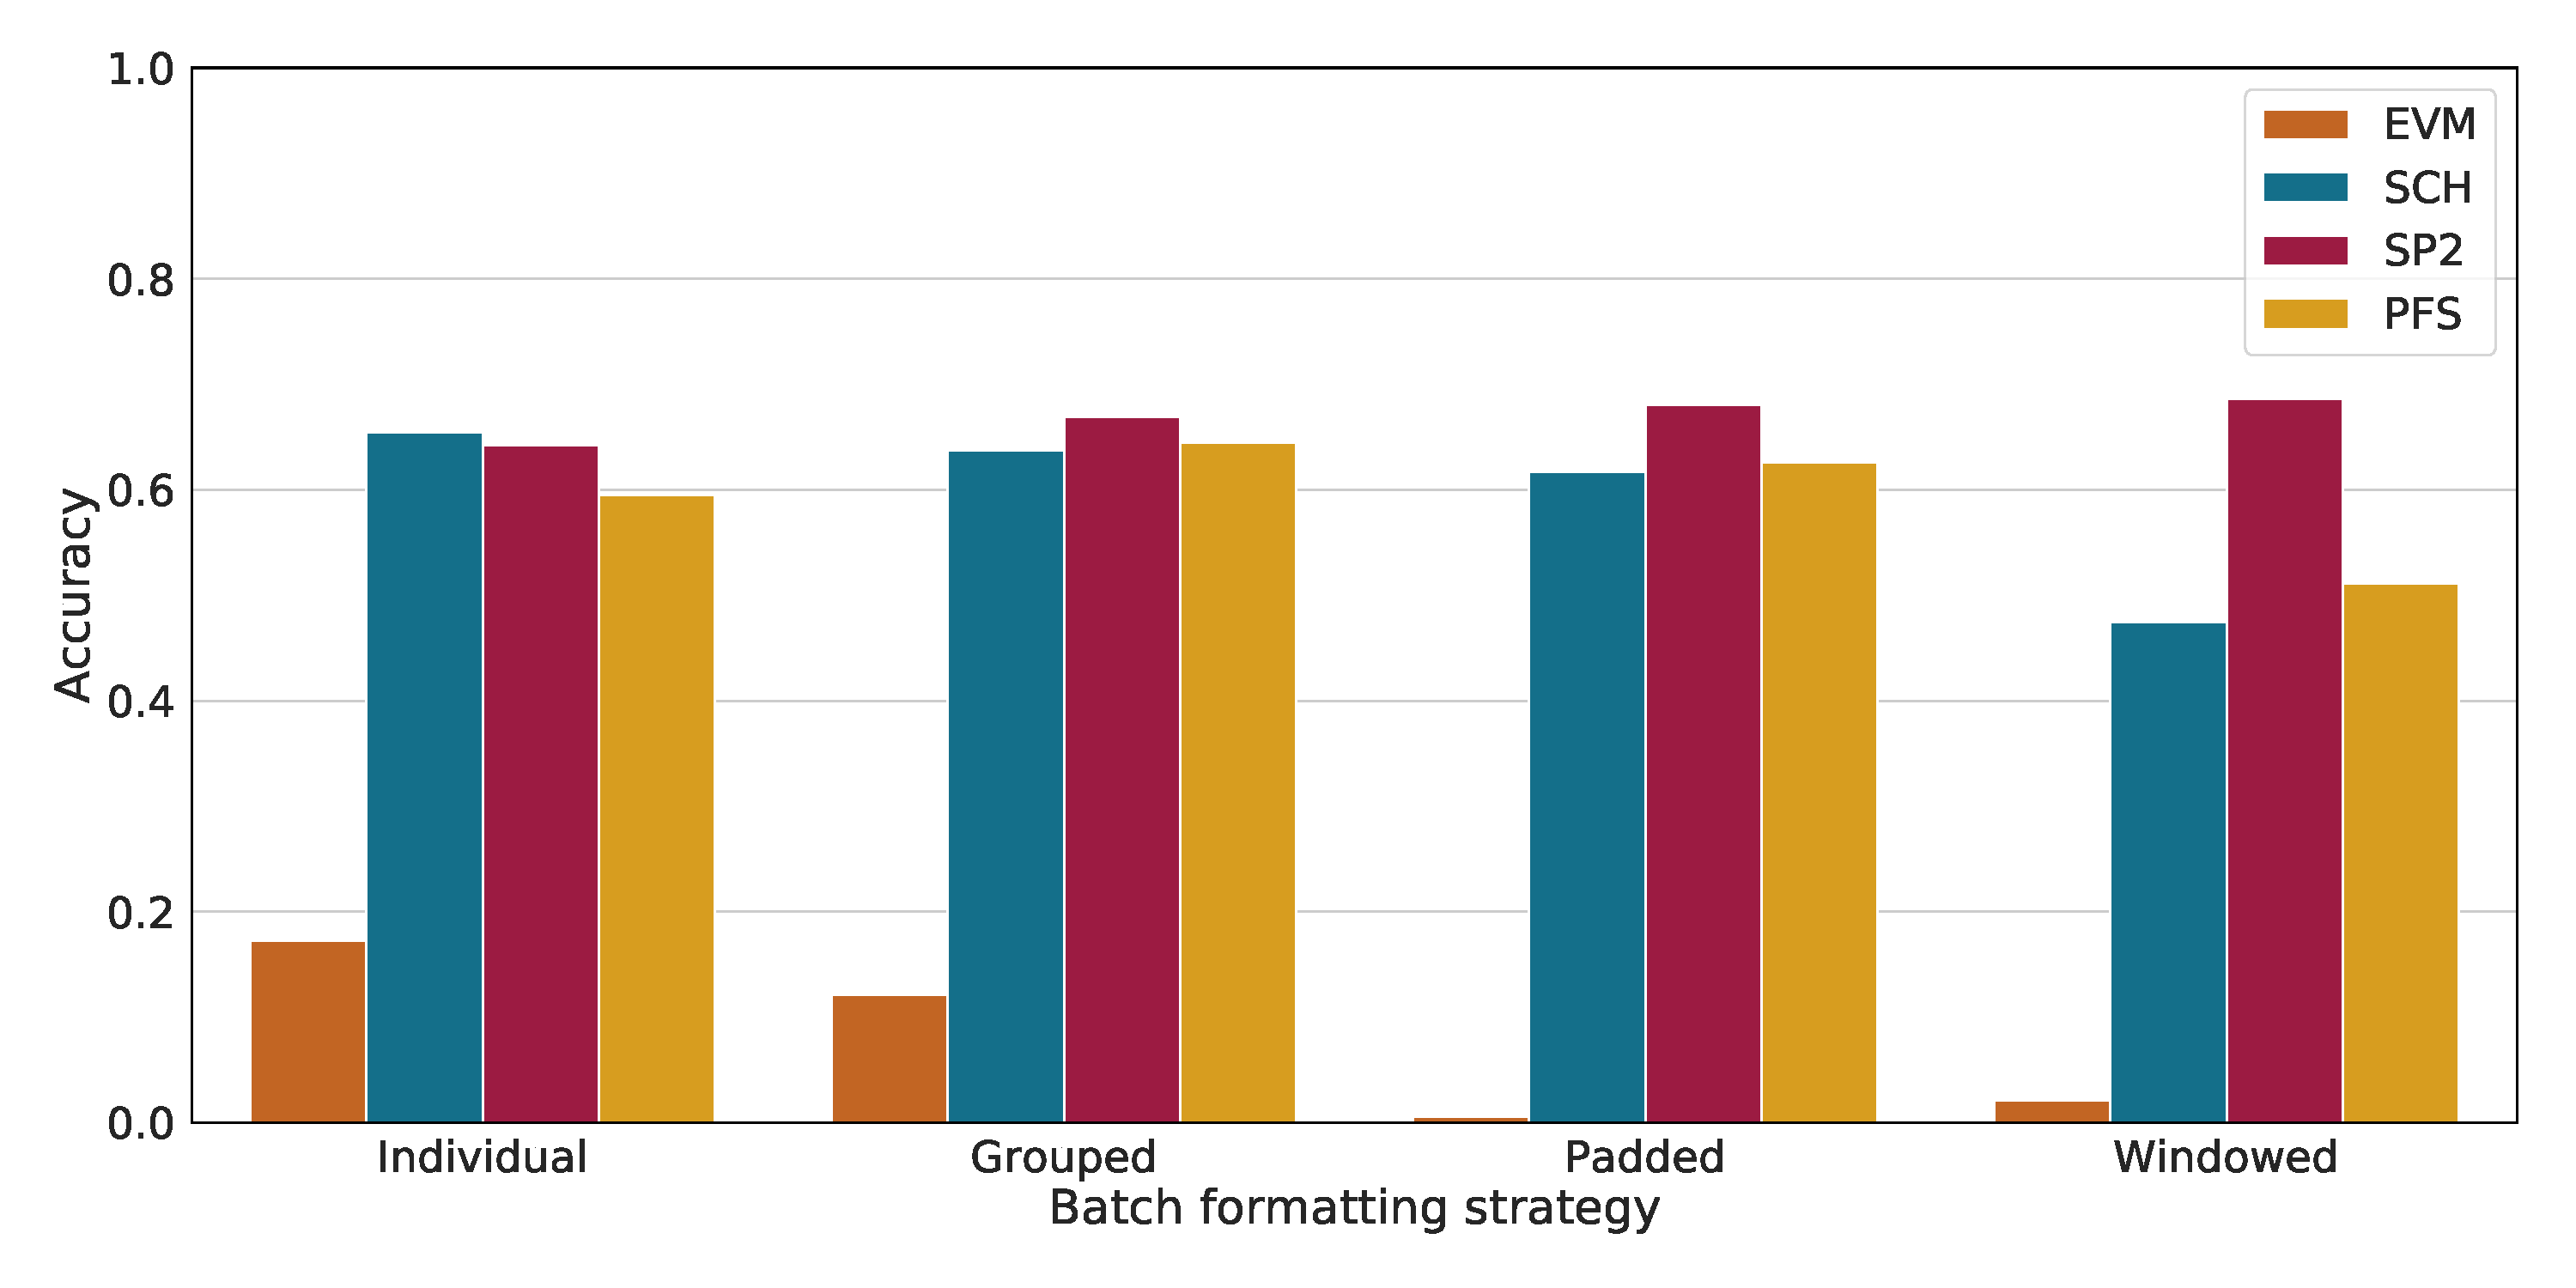
\includegraphics[width=\textwidth]{gfx/bpic2015_5/accuracies.pdf}
    \caption{Best accuracies on the validation set of BPIC15-5}
    \label{fig:max-accuracies-bpic2015-5}
\end{figure}

\paragraph{Accuracy on BPIC11}
The most complex process is captured by BPIC11.
The validation accuracies that we obtained for this log are depicted in \autoref{fig:max-accuracies-bpic2011}.

Again, the EVM model shows subpar accuracies below $0.2$ across all batching strategies.
The SCH, SP2 and PFS models are very similar on the grouping and padding strategies, with all accuracies above $0.6$.
Only with the individual strategy does the SP2 model show a severe accuracy degradation.
On this strategy, the SCH model gives the highest accuracy for this strategy with $0.682$.

\begin{figure}[!htb]
    \centering
    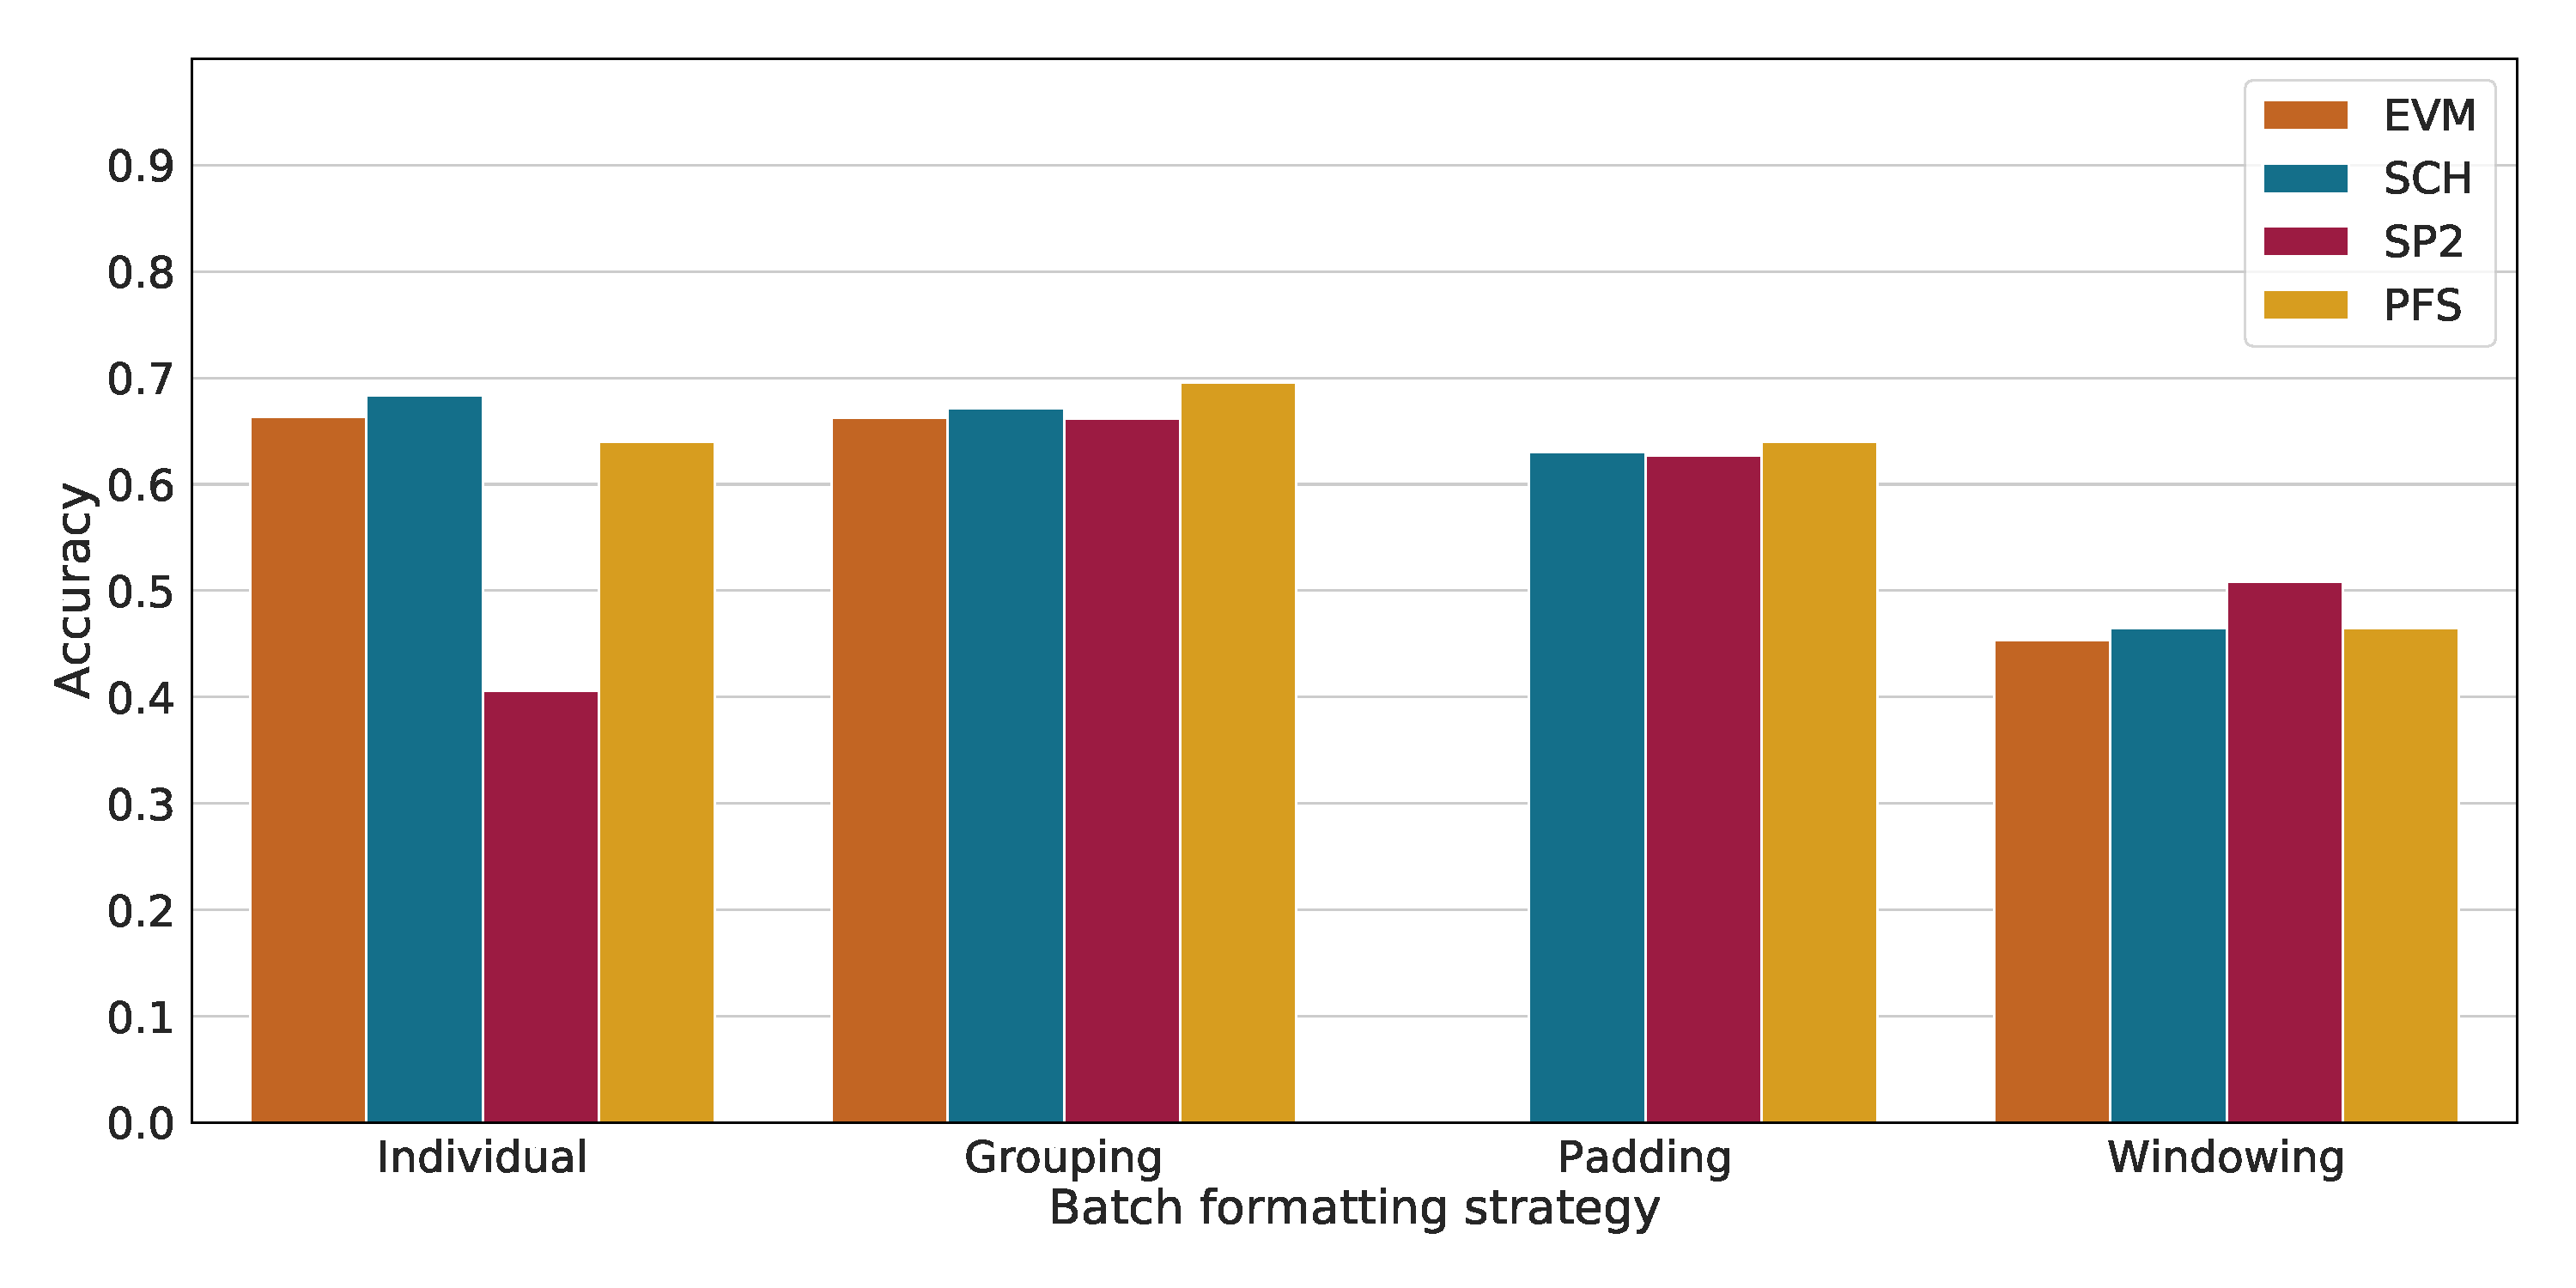
\includegraphics[width=\textwidth]{gfx/bpic2011/accuracies.pdf}
    \caption{Best accuracies on the validation set of BPIC11}
    \label{fig:max-accuracies-bpic2011}
\end{figure}

\paragraph{Verdict on accuracy}
% grouping strategy
The grouping strategy generally leads to top performance in lieu with our SP2 model on any dataset except for BPIC11 and BPIC12. On BPIC11, the strategy brings the best accuracy with the PFS model. On BPIC12, it leads to the worst accuracies. The explanation for this can be found in \autoref{tab:dataset-characteristics} and \autoref{tab:batch-sizes}. The dataset has the highest number of traces, and a relatively even distribution of lengths, resulting in a small standard deviation. This results in too many traces being put into a single batch, causing lost optimization opportunities. With this in mind, the grouping strategy should be enhanced to split batches if they exceed a certain size threshold. Nonetheless, we realized that the mean of the top accuracies of the SCH, SP2 and PFS models is the highest with the grouping strategy. \autoref{tab:strategy-top-accuracies} illustrates these mean accuracies.

The table on mean accuracies also reveals that the prediction accuracy goes down with increasing complexity of the process.
It is most accurate on the HelpDesk process and steadily decreases toward BPIC11.

Looking at the accuracy of the EVM model across all datasets, it becomes apparent that it is consistently outperformed.
As the fundamental difference between the EVM and SCH models is an embedding layer, we suspect that the bad results can be traced back to this layer.
We believe that it requires more datapoints per class than included in most datasets to perform well.
On the HelpDesk log there is a very small number of classes, and a large number of traces, which could be a reason for the EVM model scoring above $0.720$.

\begin{table}
\centering
\begin{tabular}{lrrrr}
\textbf{Dataset}  &  \textbf{Individual} &  \textbf{Grouping} &   \textbf{Padding} &  \textbf{Windowing}\\
\midrule
\textbf{HelpDesk} &    0.855    &  0.844    &  0.832    &  0.685    \\
\textbf{BPIC12  } &    0.850    &  0.761    &  0.833    &  0.728    \\
\textbf{BPIC15-1} &    0.614    &  0.670    &  0.635    &  0.559    \\
\textbf{BPIC15-2} &    0.577    &  0.604    &  0.581    &  0.503    \\
\textbf{BPIC15-3} &    0.649    &  0.680    &  0.654    &  0.581    \\
\textbf{BPIC15-4} &    0.638    &  0.668    &  0.645    &  0.579    \\
\textbf{BPIC15-5} &    0.630    &  0.650    &  0.640    &  0.557    \\
\textbf{BPIC11  } &    0.576    &  0.676    &  0.632    &  0.479    \\
\end{tabular}
\caption[Grouping strategy leads to best mean accuracies]{Accuracy means across the top accuracies of the SCH, SP2 and PFS models. The grouping strategy is generally the highest}
\label{tab:strategy-top-accuracies}
\end{table}
\FloatBarrier

\section{Training time}\label{sec:eval:training-time}
The training time that a model requires for an epoch is important to gauge the efficiency of its training process.
As in the previous section, we will discuss the measurements per log, and finish with a verdict.
For each log, a plot is shown that presents the training time per model, grouped by batching strategy.
The plots do not share the same scale on the y-axis.
During the following paragraphs it is important to keep in mind that the batch size has a direct effect on the training time since it corresponds to the number of weight adjustments that need to be calculated.

\paragraph{Training times on HelpDesk}
How long training an epoch took with a model and a certain strategy is shown in \autoref{fig:helpdesk-training-timings}.
Training for an epoch takes the least amount of time with the grouping strategy, and the most with the individual strategy.
The timings are very similar for all models on the same strategy.

\begin{figure}[!htb]
    \centering
    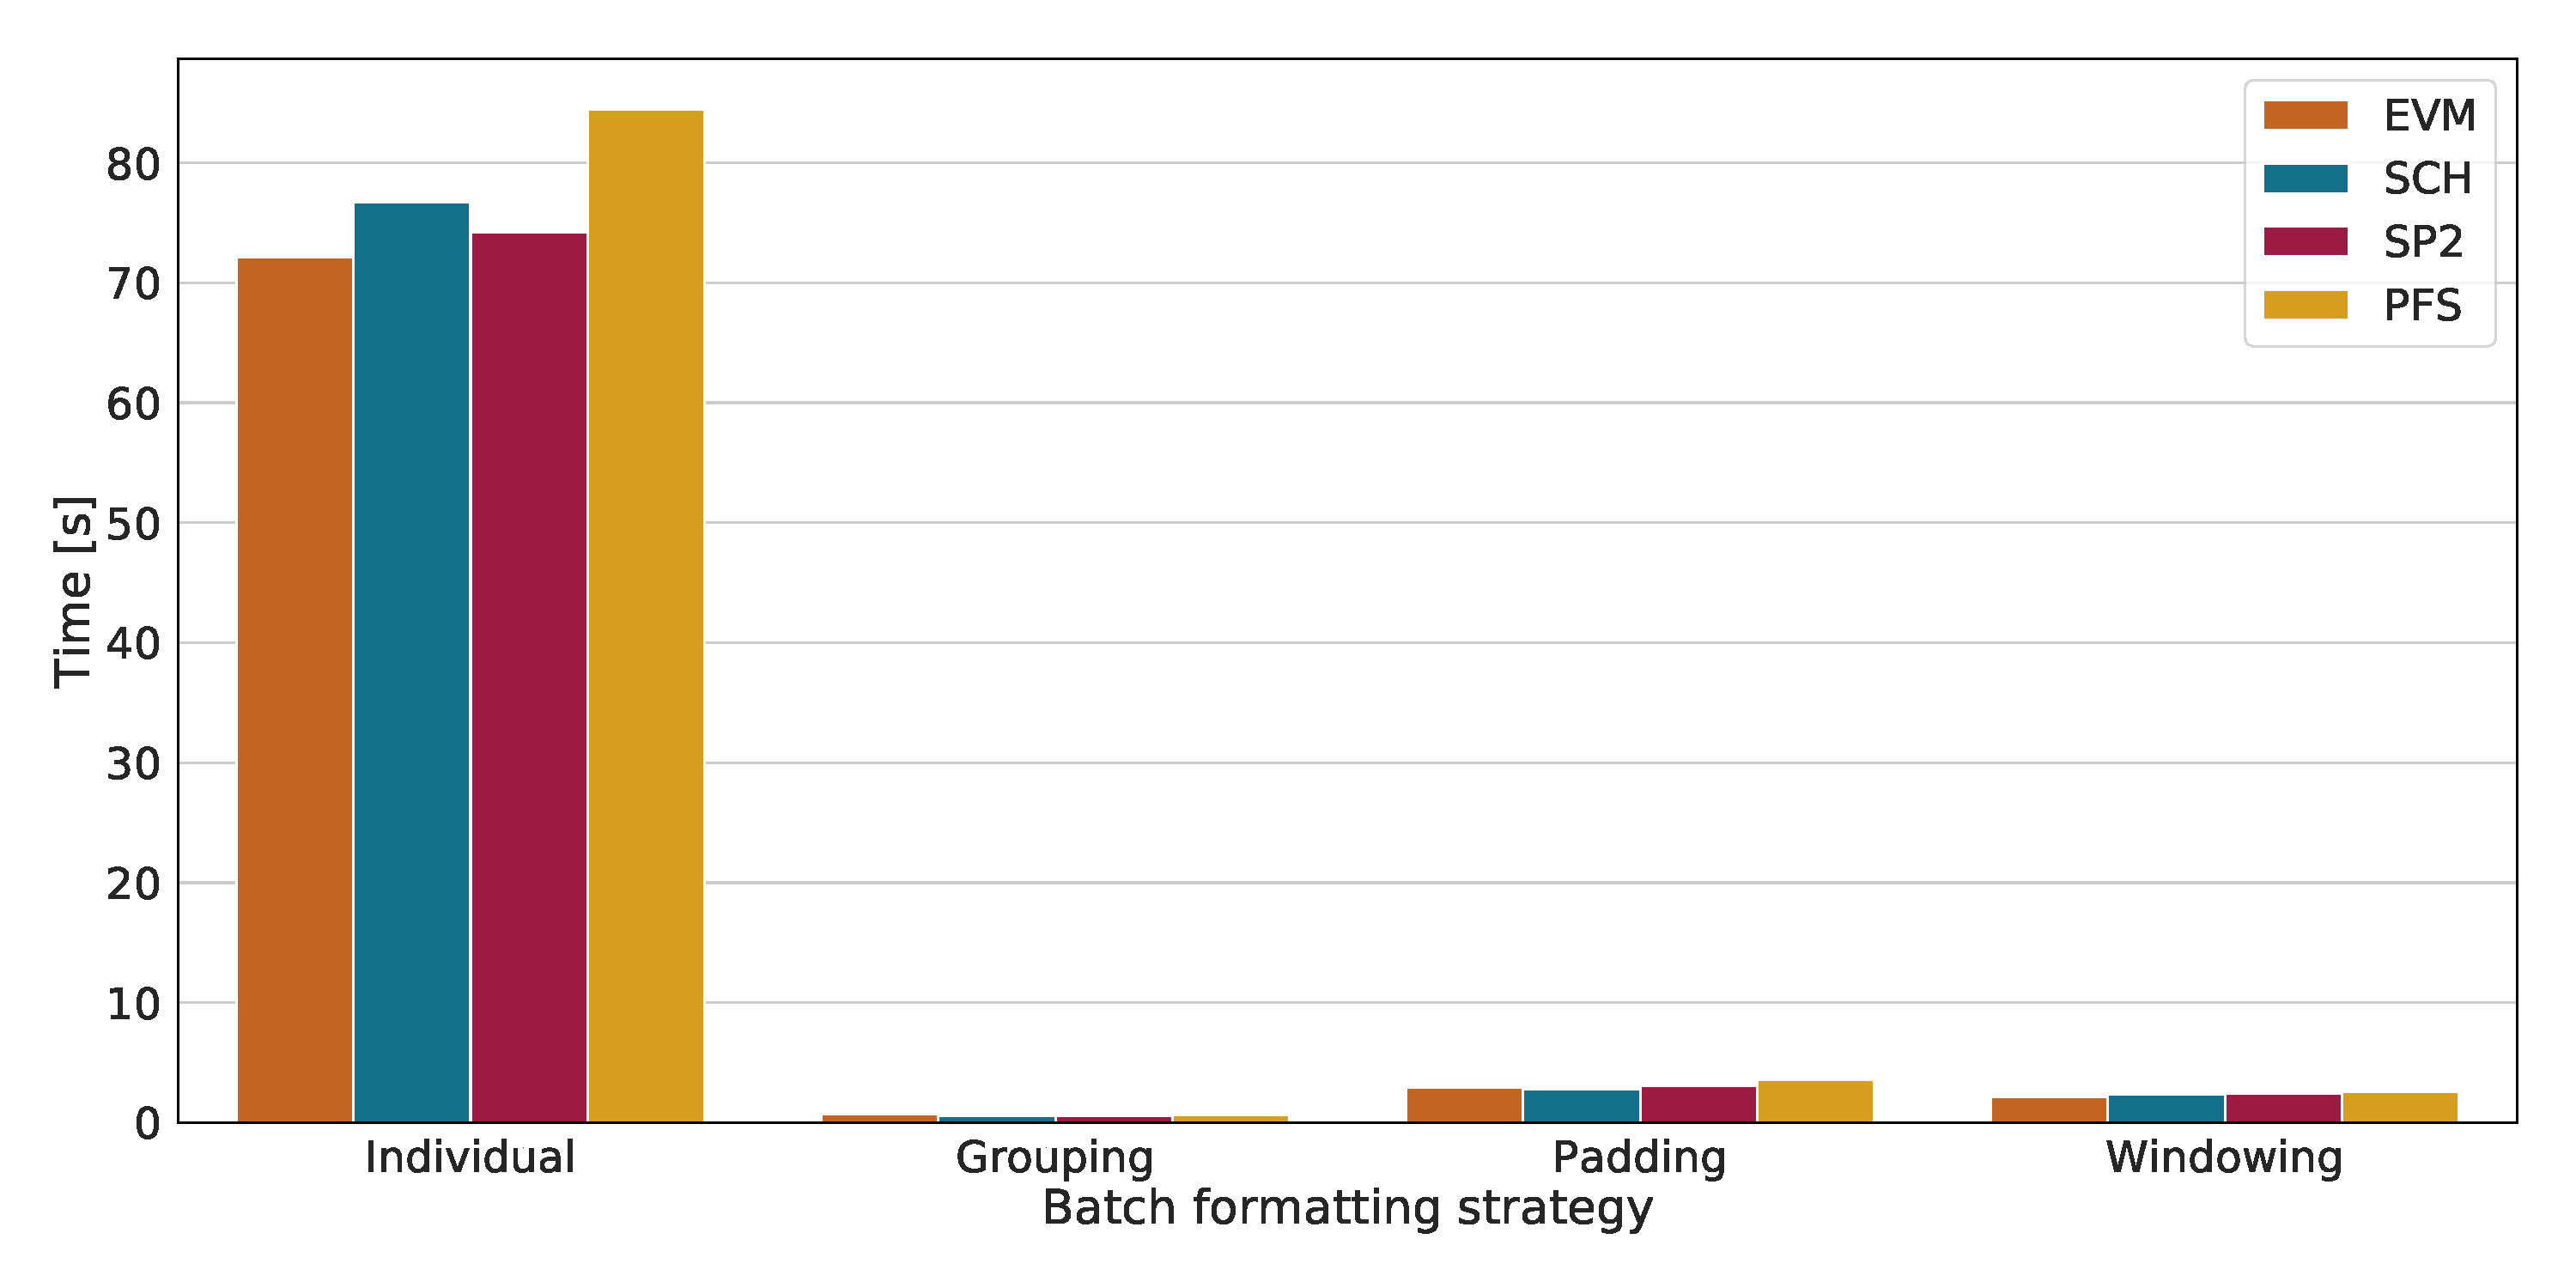
\includegraphics[width=\textwidth]{gfx/helpdesk/train_timings.pdf}
    \caption{Training times measured on HelpDesk}
    \label{fig:helpdesk-training-timings}
\end{figure}

\paragraph{Training times on BPIC12}
\autoref{fig:BPIC12-training-timings} depicts the epoch training times for BPIC12.
As for the HelpDesk log, the timings for models on the same strategy are very similar.
By far, they are the highest for each model on the individual strategy at approximately 10 minutes.
The other strategies take significantly less time.

\begin{figure}[!htb]
    \centering
    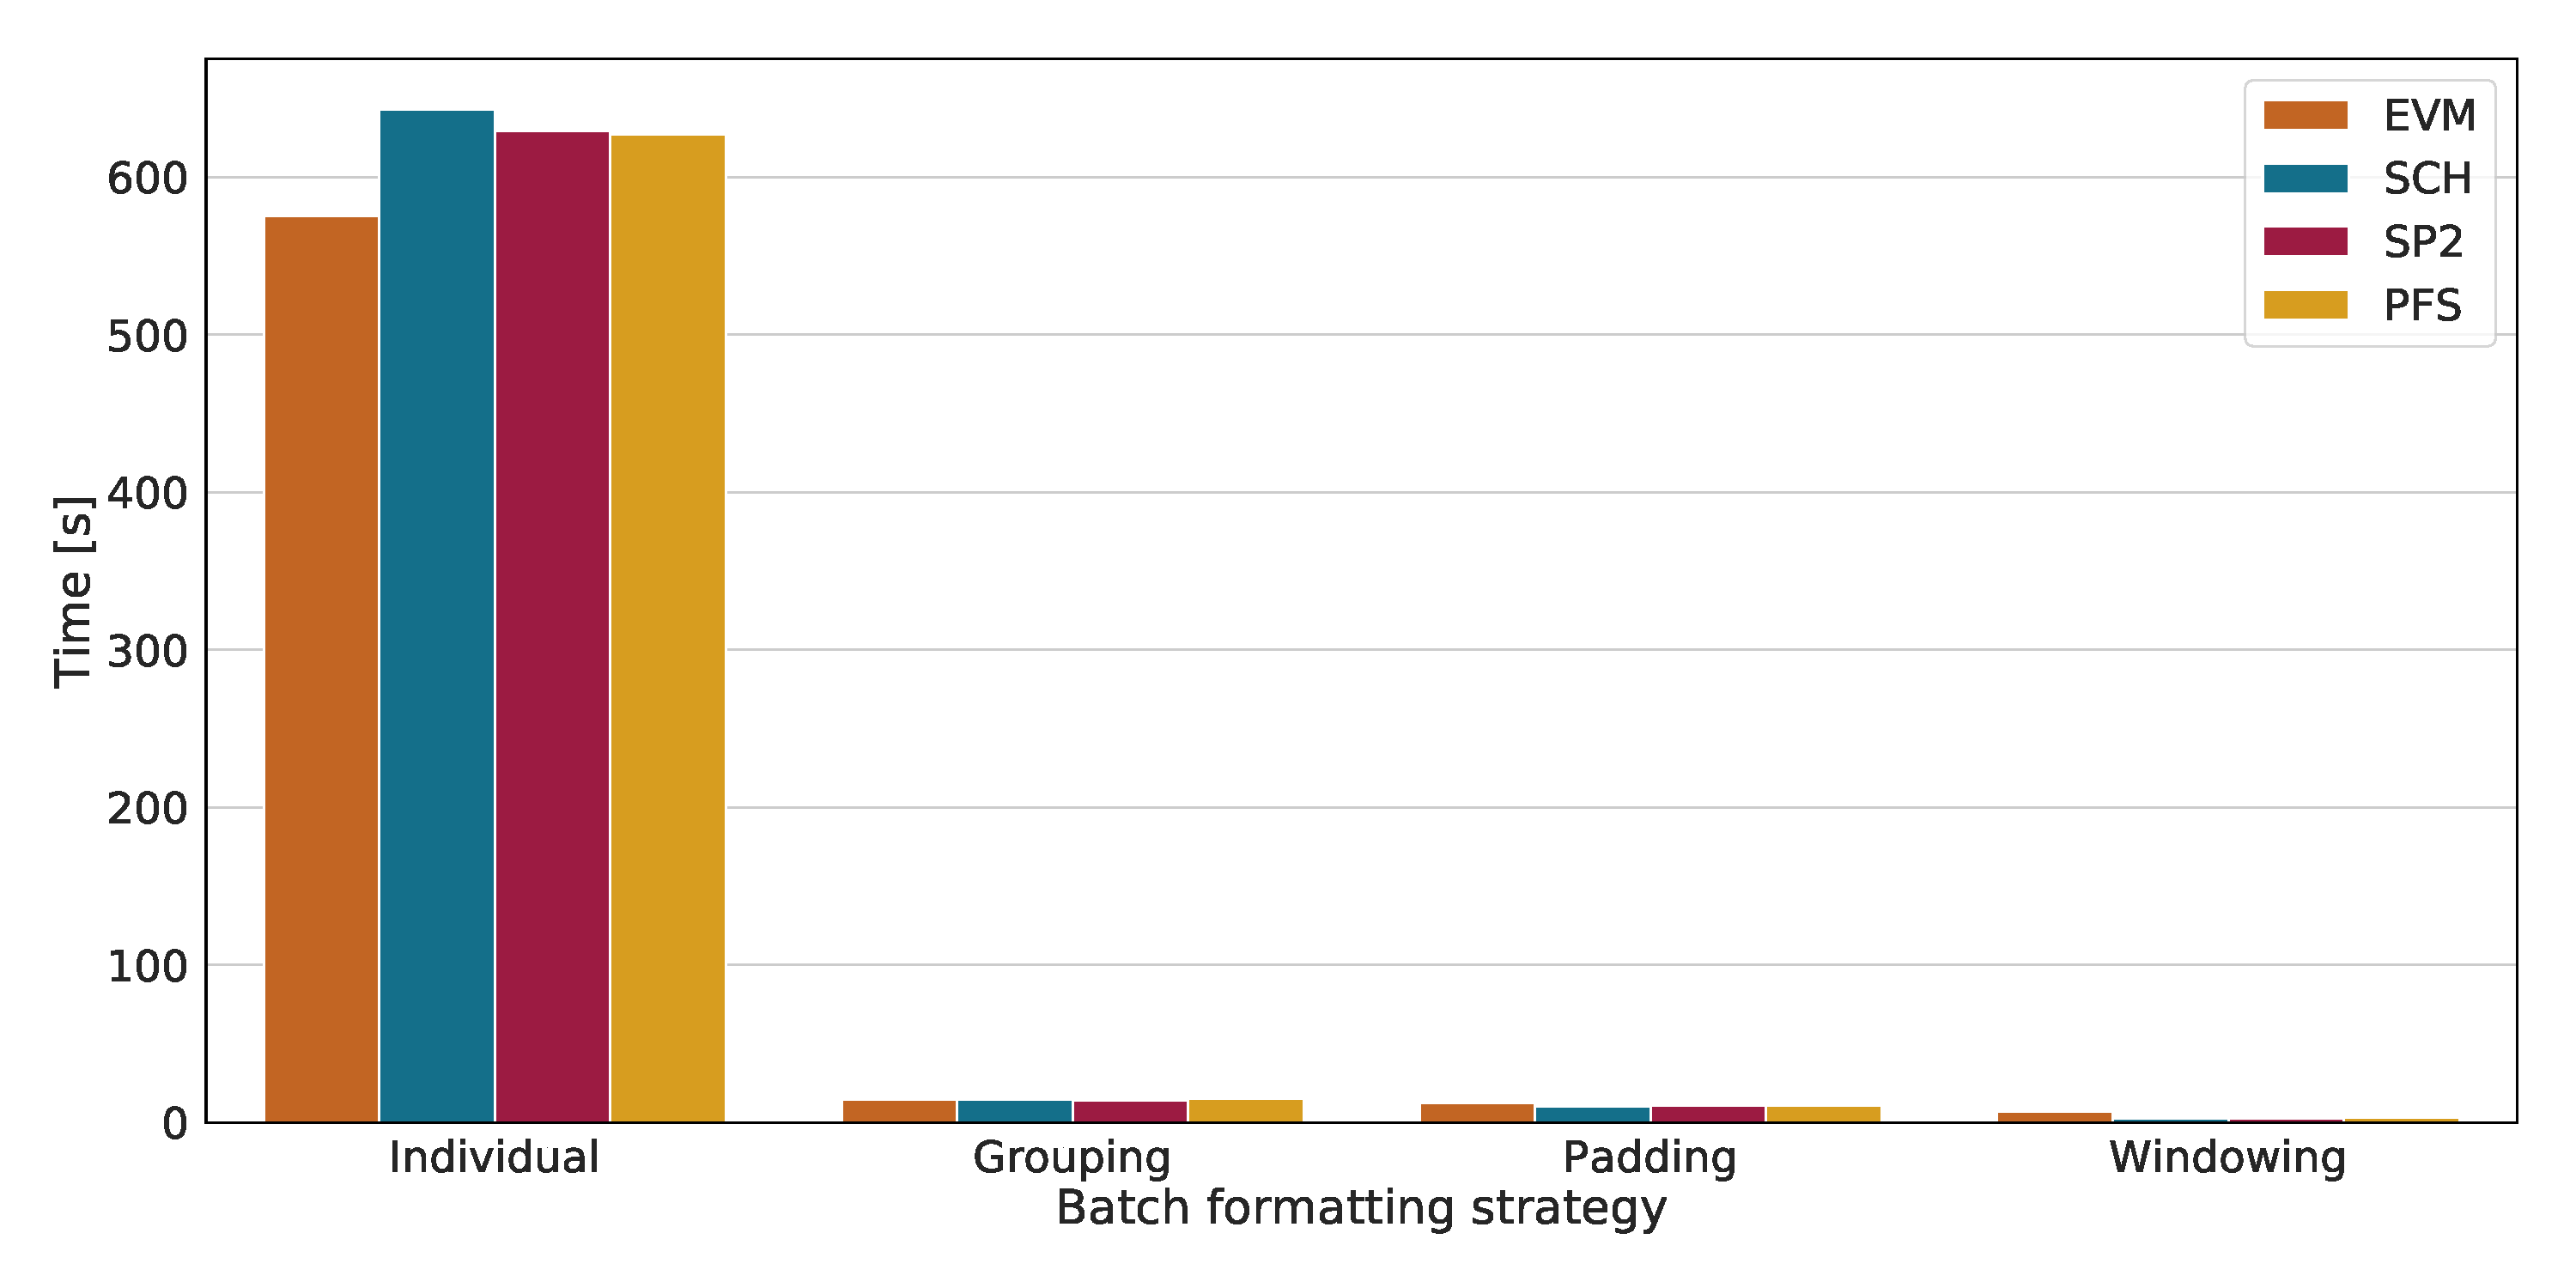
\includegraphics[width=\textwidth]{gfx/bpic2012/train_timings.pdf}
    \caption{Training times measured on BPIC12}
    \label{fig:BPIC12-training-timings}
\end{figure}

\paragraph{Training times on BPIC15}
The training timings taken during the training of the BPIC15 log datasets are shown in \autoref{fig:BPIC15-1-training-timings} to \autoref{fig:BPIC15-5-training-timings}.

As before with accuracy, the SCH, SP2 and PFS models always need a very similar amount of training time per epoch.
The EVM model needs often less than half that time.
Across all five datasets it is also possible to see that the individual strategy takes by far the most time.
Significantly less time is needed by the padding strategy, although it still ranks third.
The grouping strategy needs a little less time, and the windowing strategy trains fastest by far.

\begin{figure}[!htb]
    \centering
    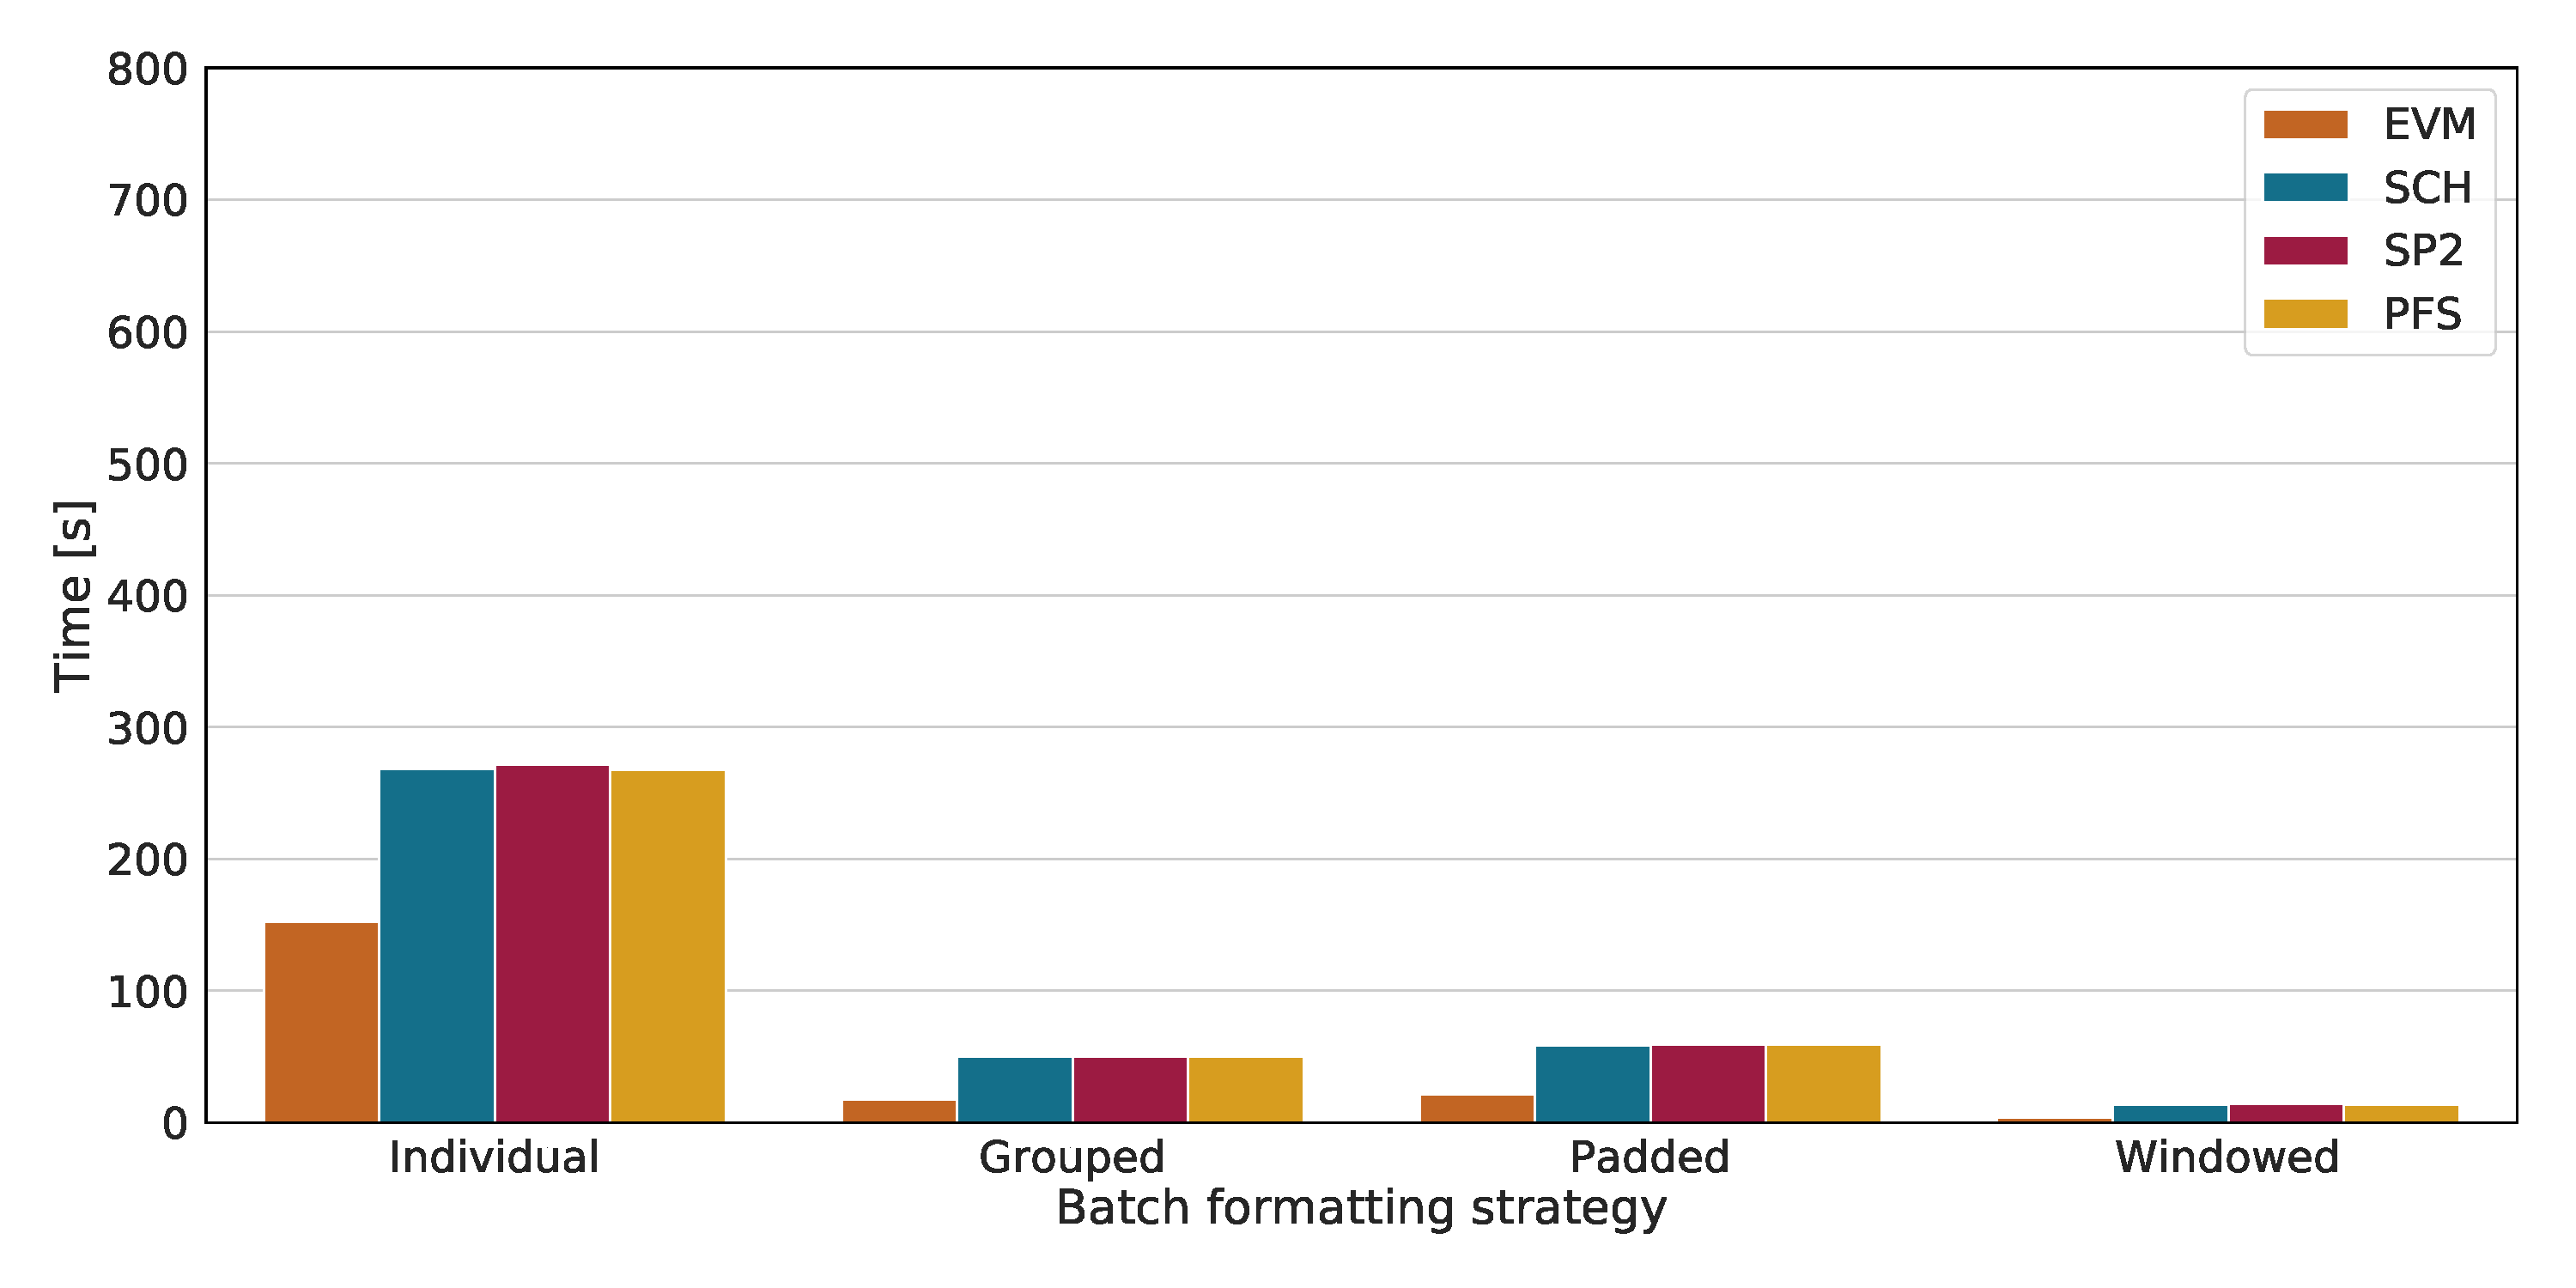
\includegraphics[width=\textwidth]{gfx/bpic2015_1/train_timings.pdf}
    \caption{Training times measured on BPIC15-1}
    \label{fig:BPIC15-1-training-timings}
\end{figure}
\begin{figure}[!htb]
    \centering
    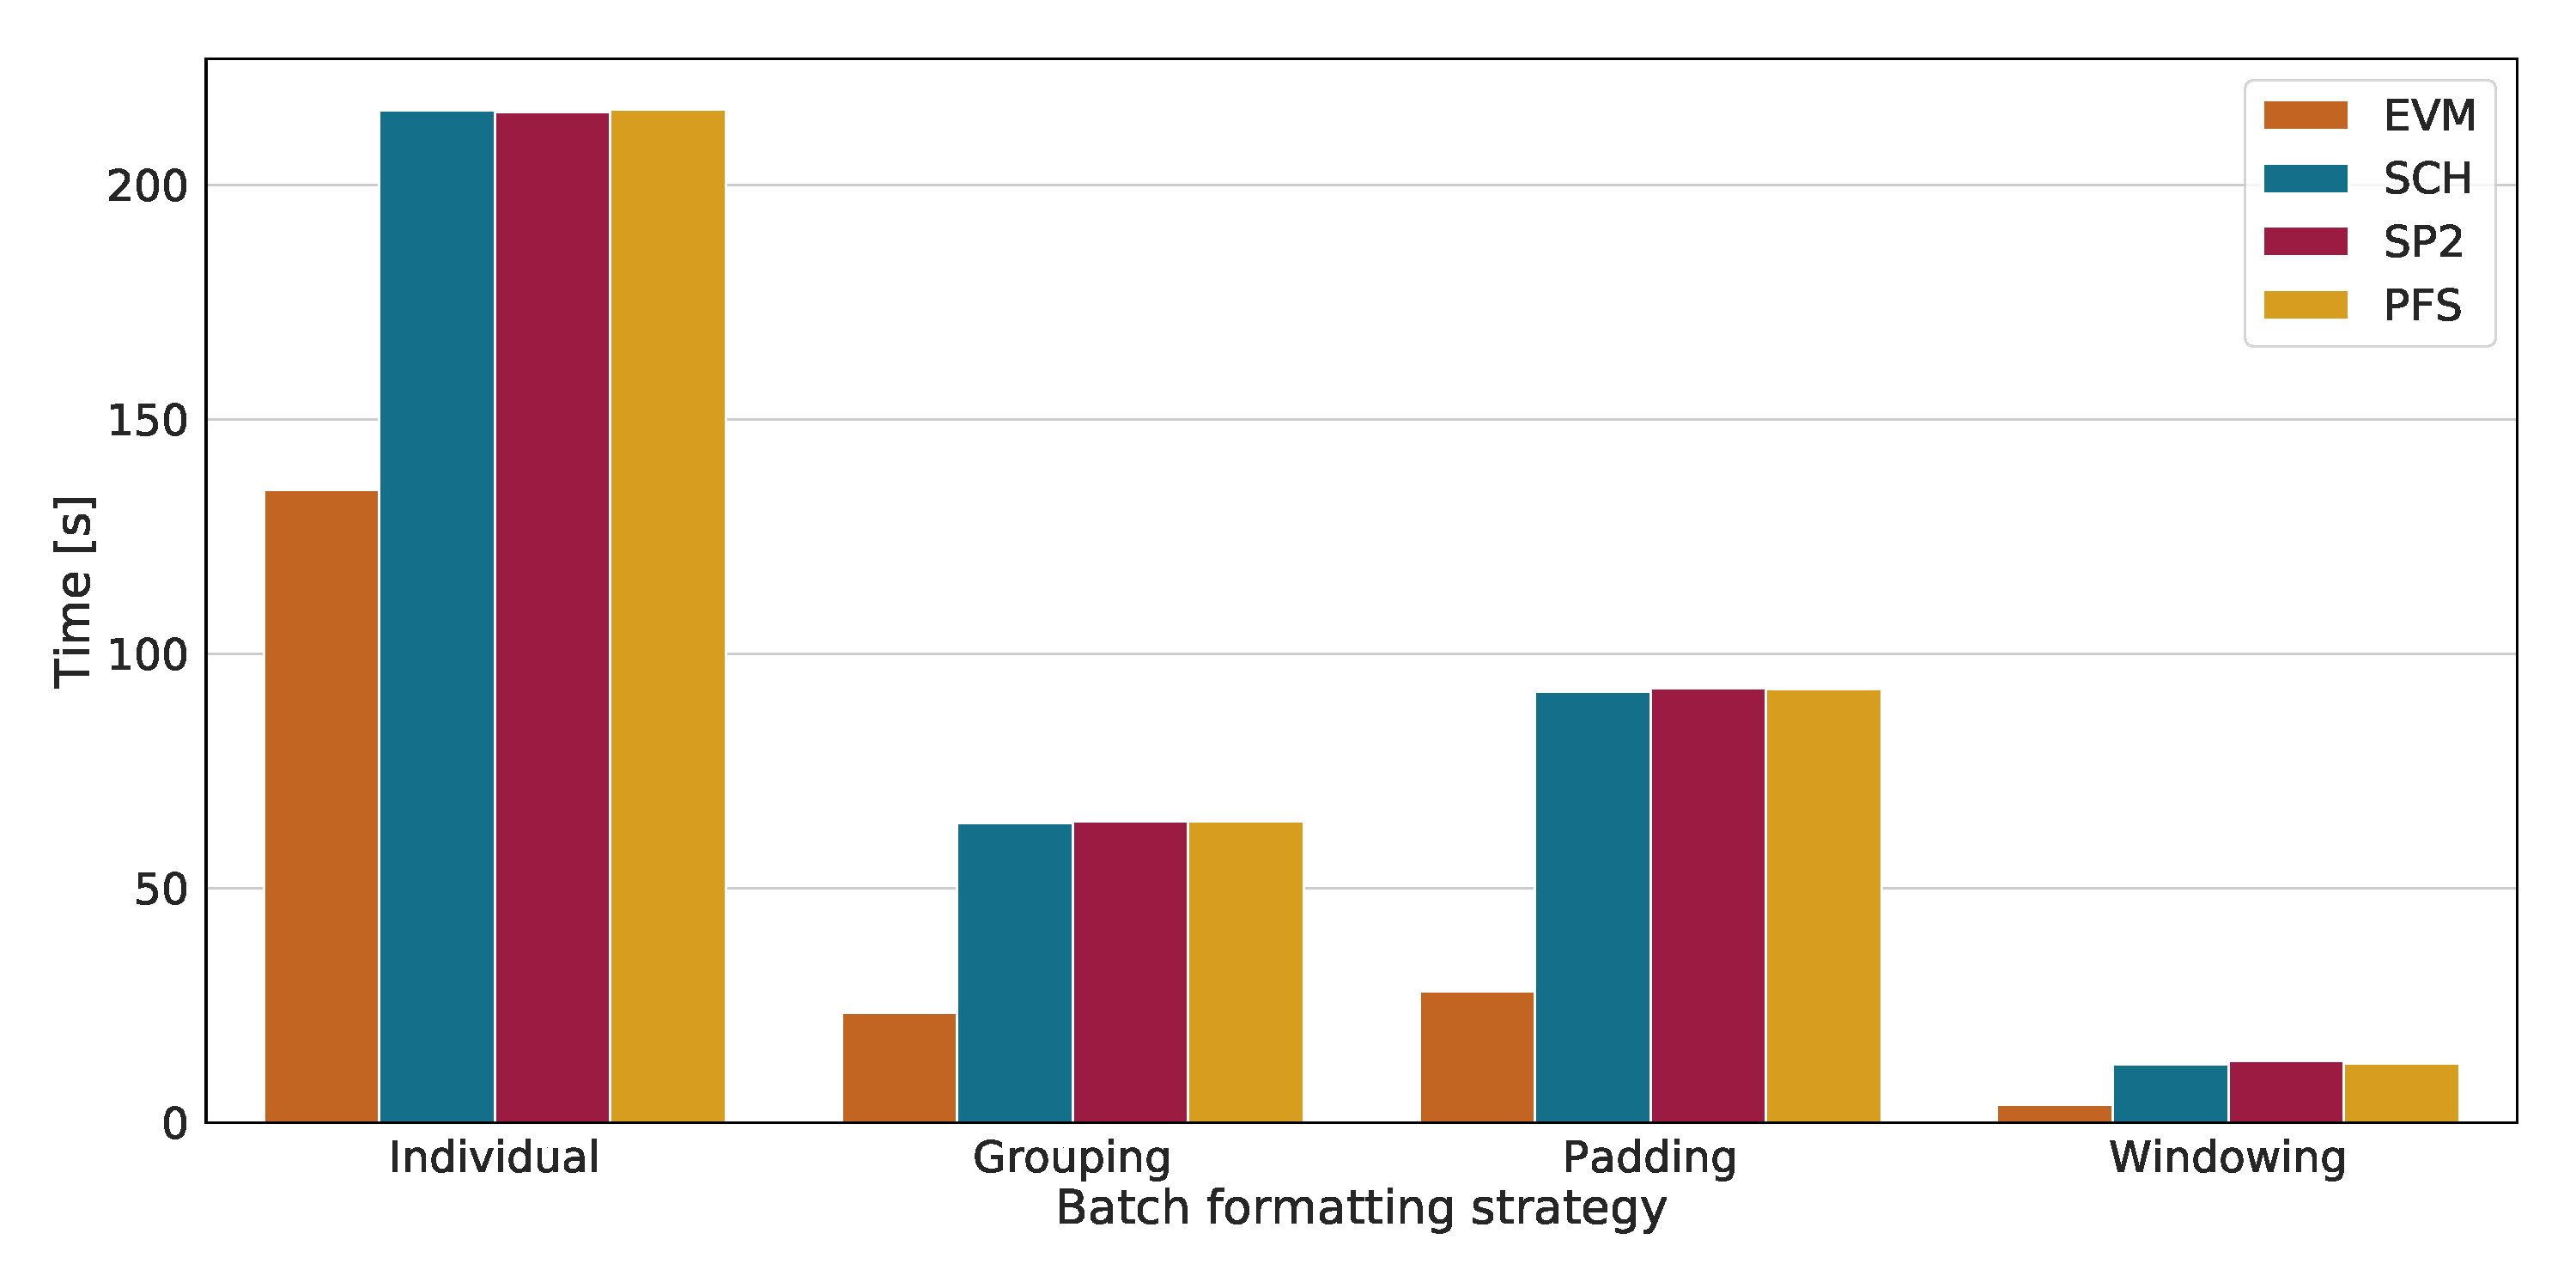
\includegraphics[width=\textwidth]{gfx/bpic2015_2/train_timings.pdf}
    \caption{Training times measured on BPIC15-2}
    \label{fig:BPIC15-2-training-timings}
\end{figure}
\begin{figure}[!htb]
    \centering
    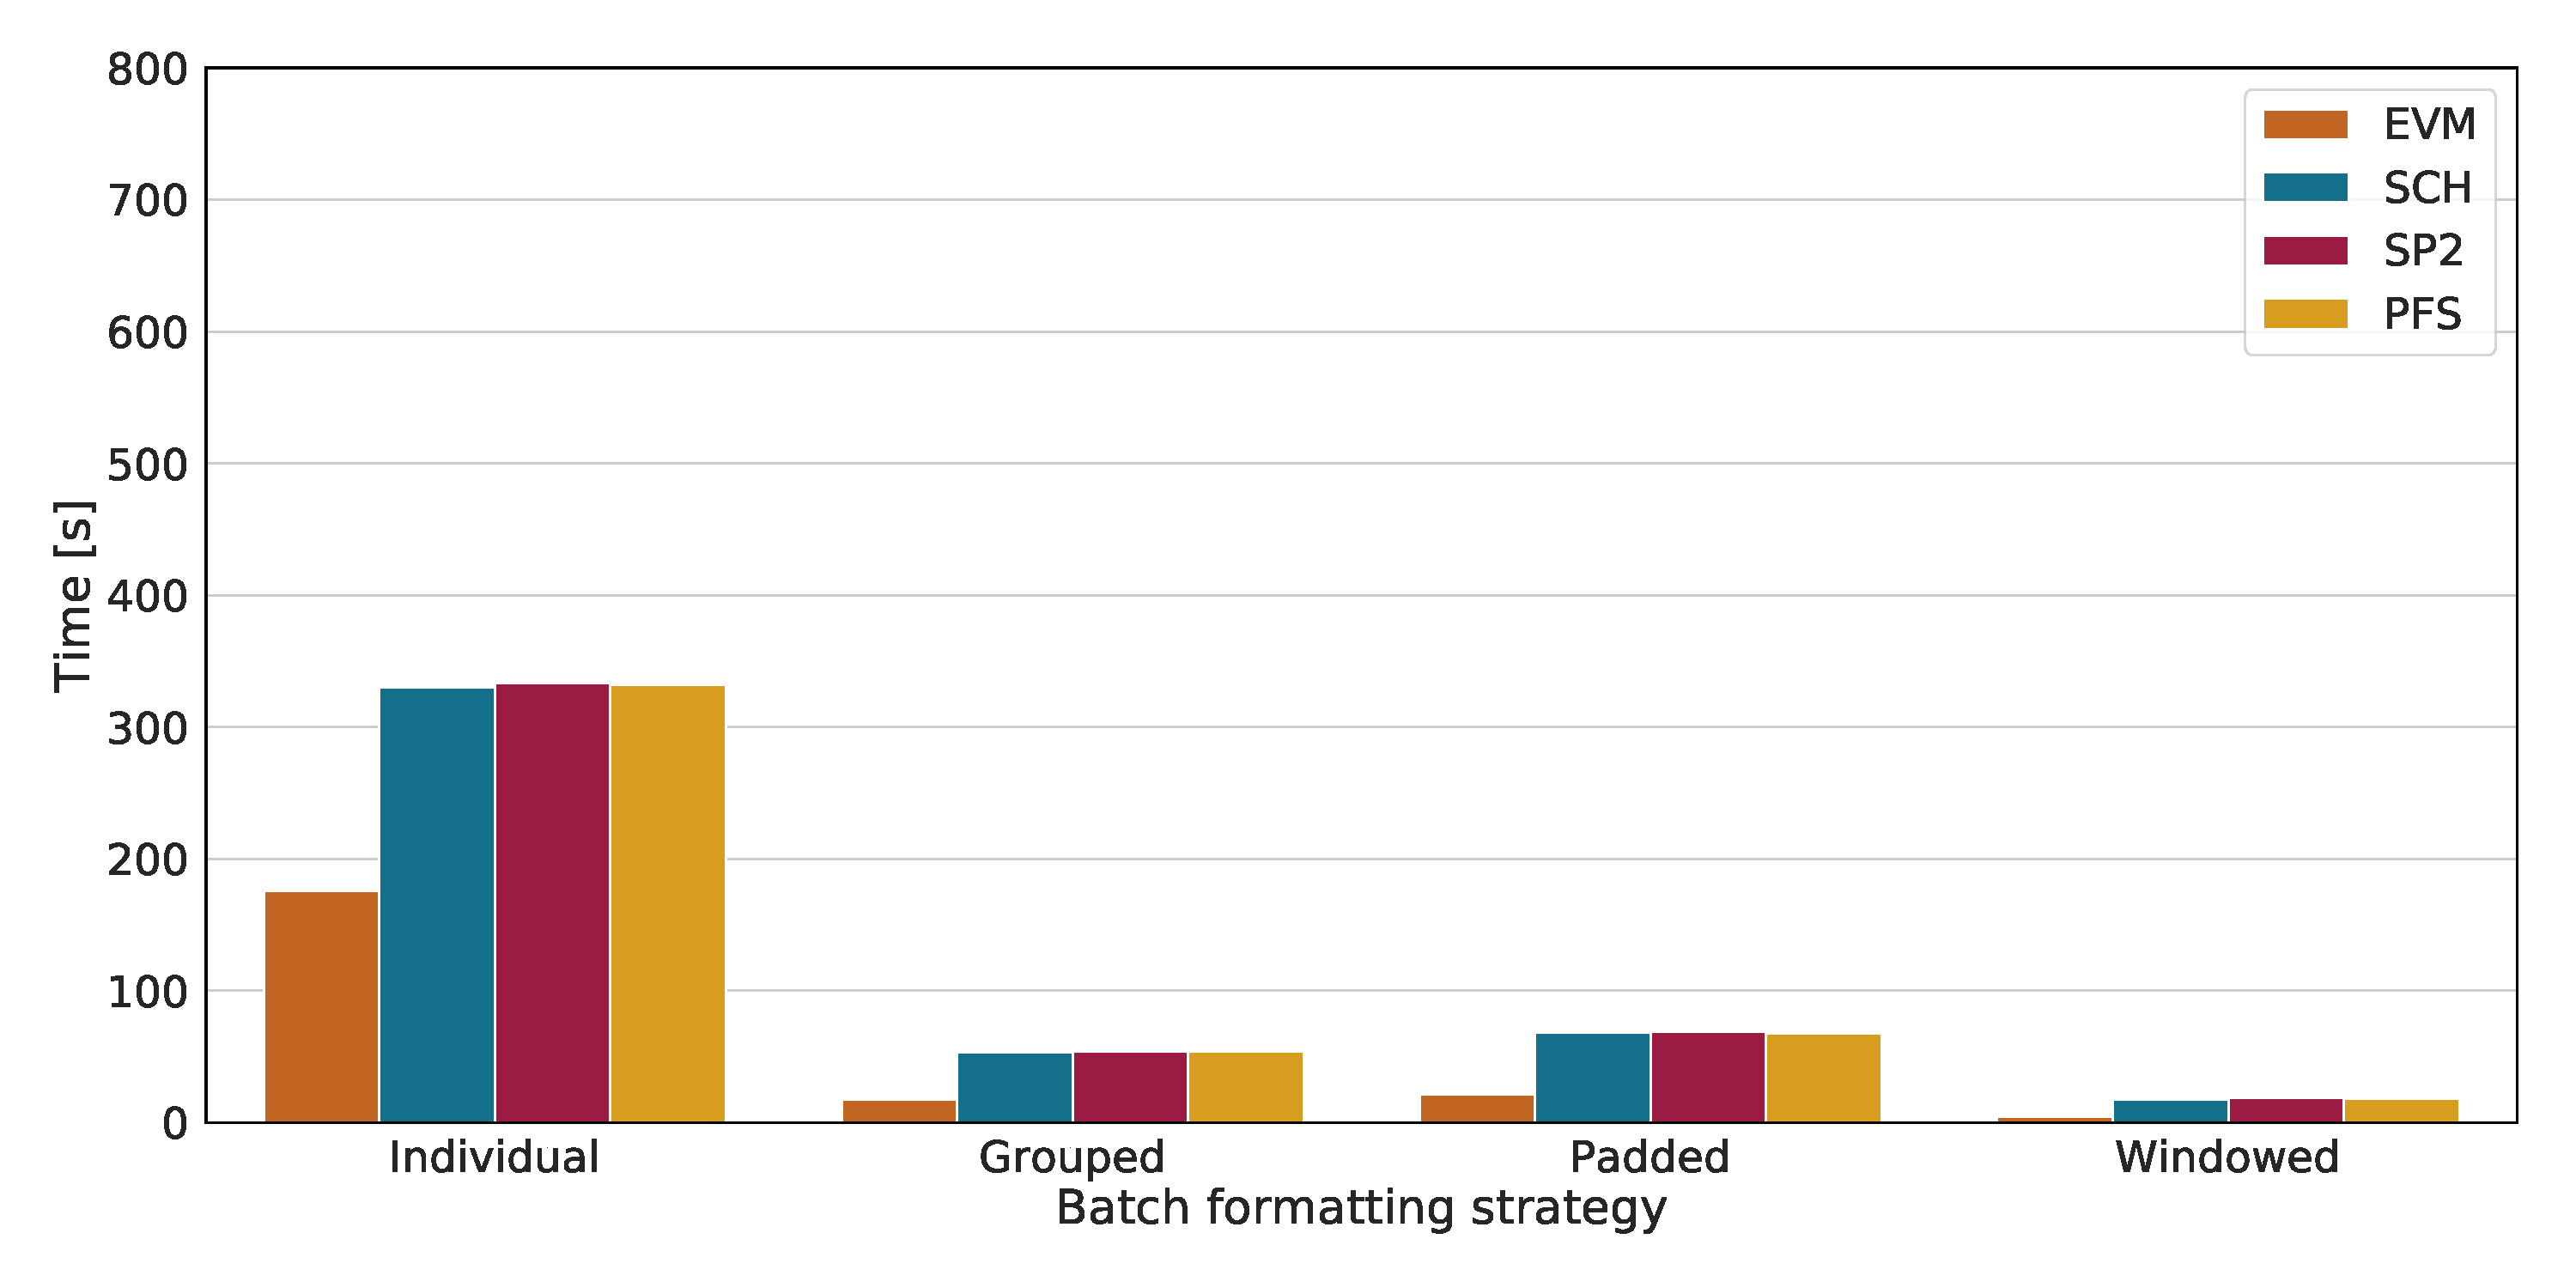
\includegraphics[width=\textwidth]{gfx/bpic2015_3/train_timings.pdf}
    \caption{Training times measured on BPIC15-3}
    \label{fig:BPIC15-3-training-timings}
\end{figure}
\begin{figure}[!htb]
    \centering
    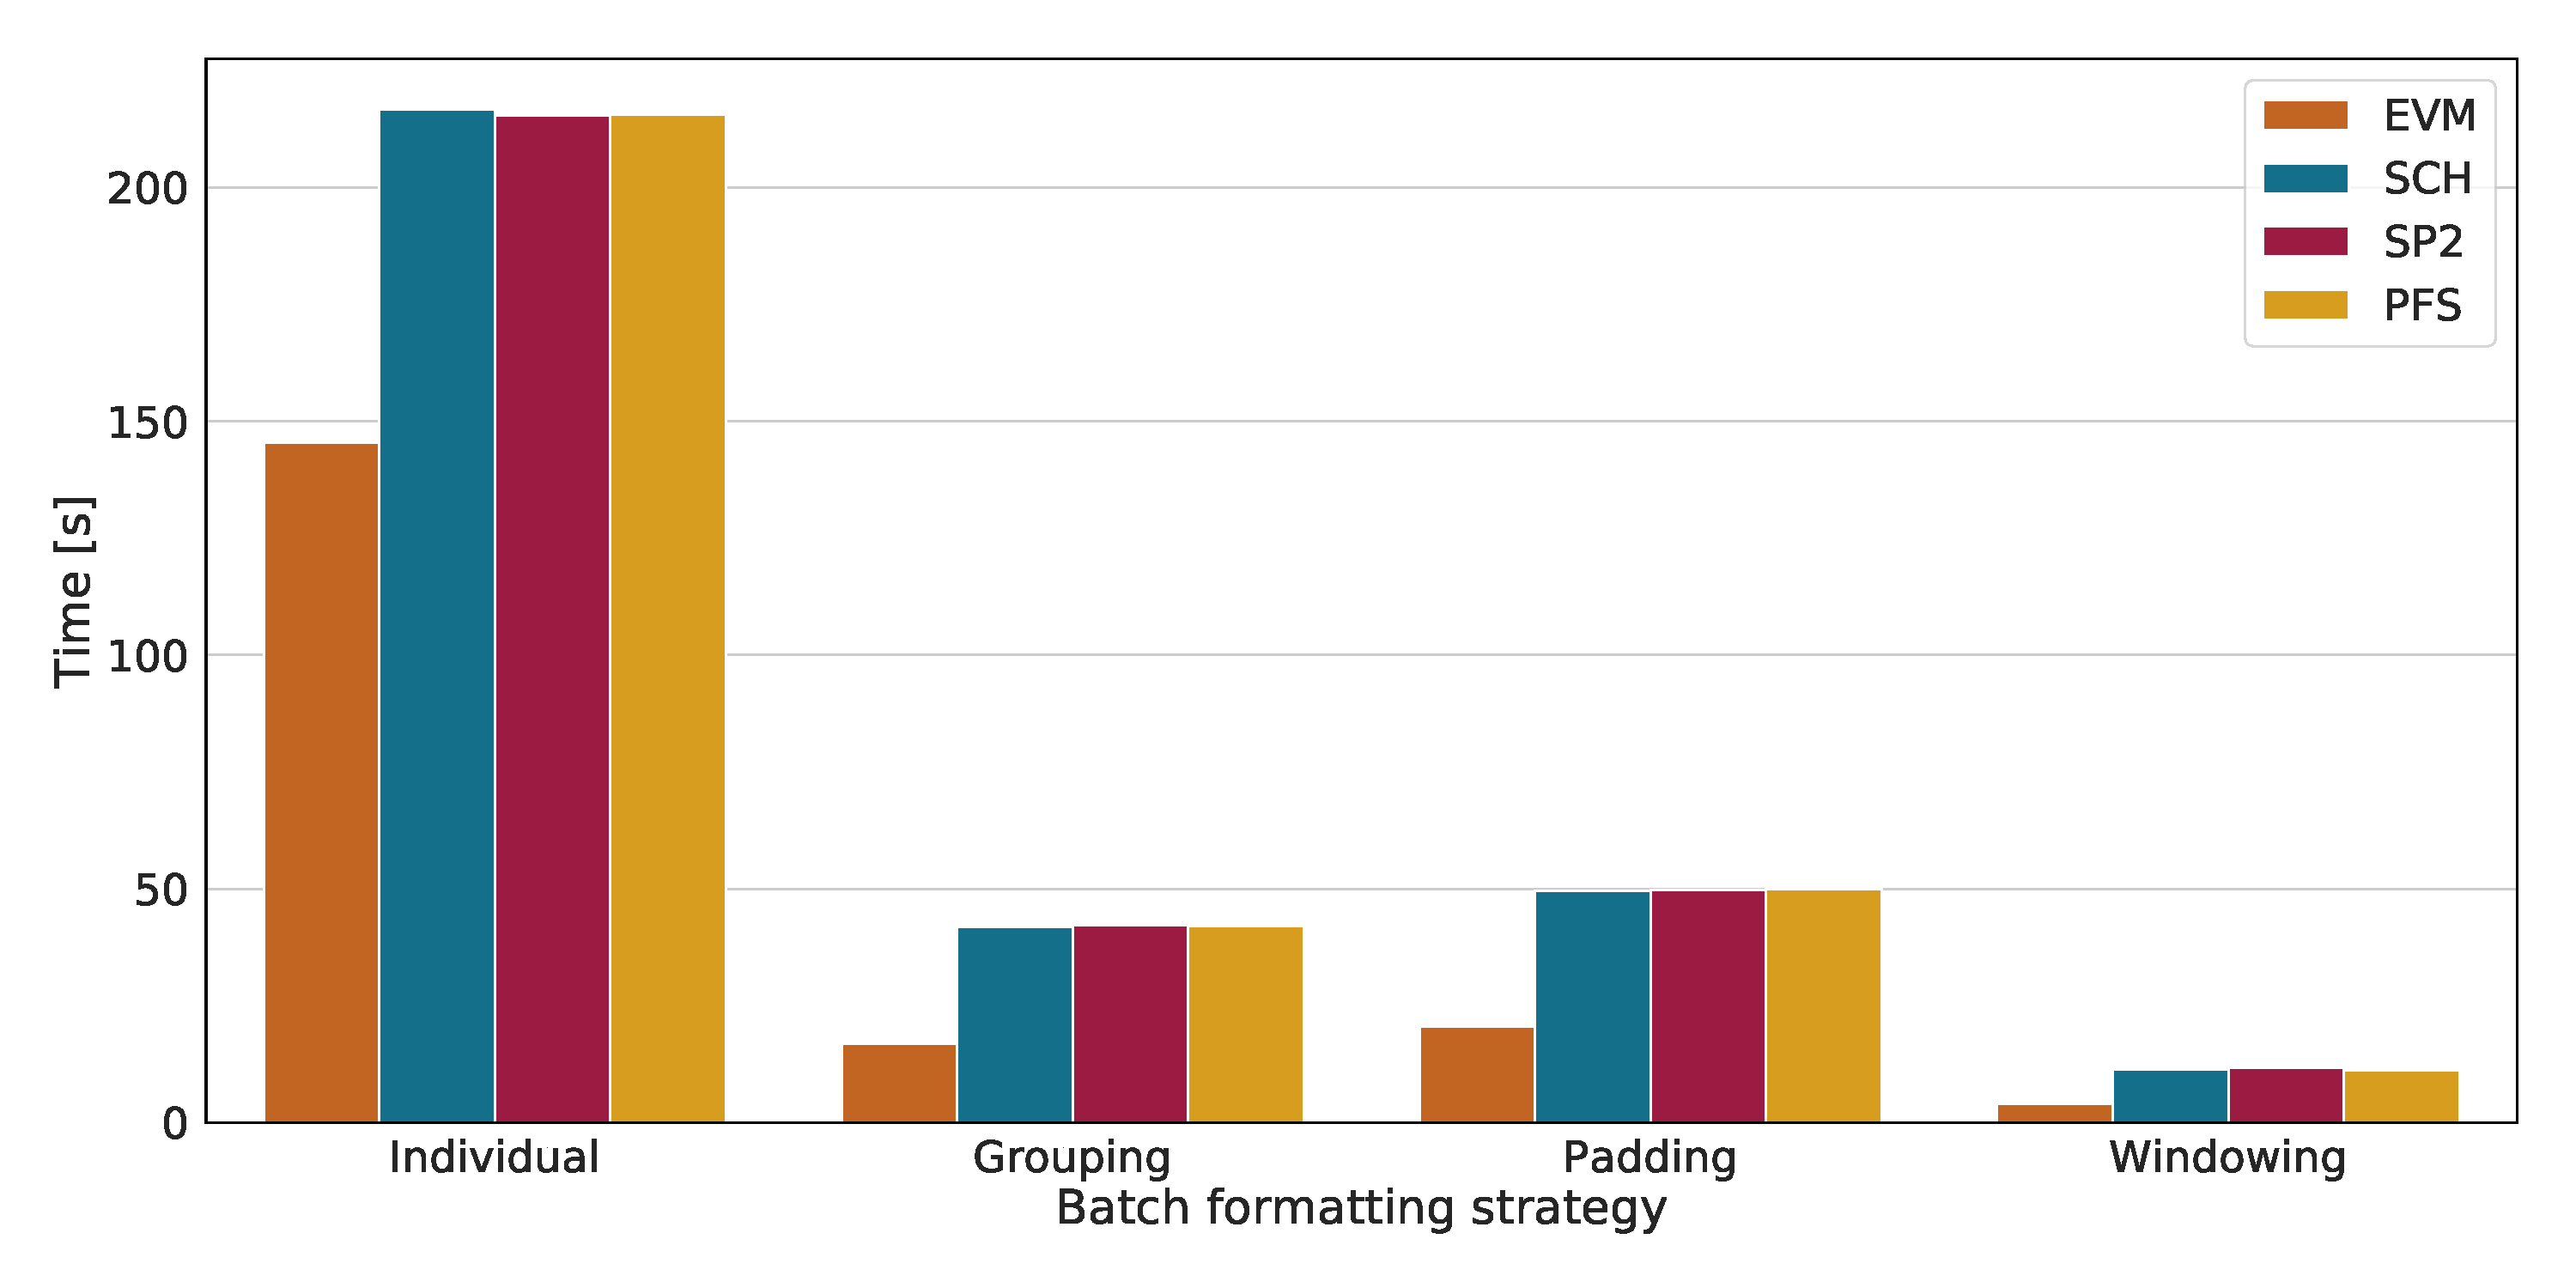
\includegraphics[width=\textwidth]{gfx/bpic2015_4/train_timings.pdf}
    \caption{Training times measured on BPIC15-4}
    \label{fig:BPIC15-4-training-timings}
\end{figure}
\begin{figure}[!htb]
    \centering
    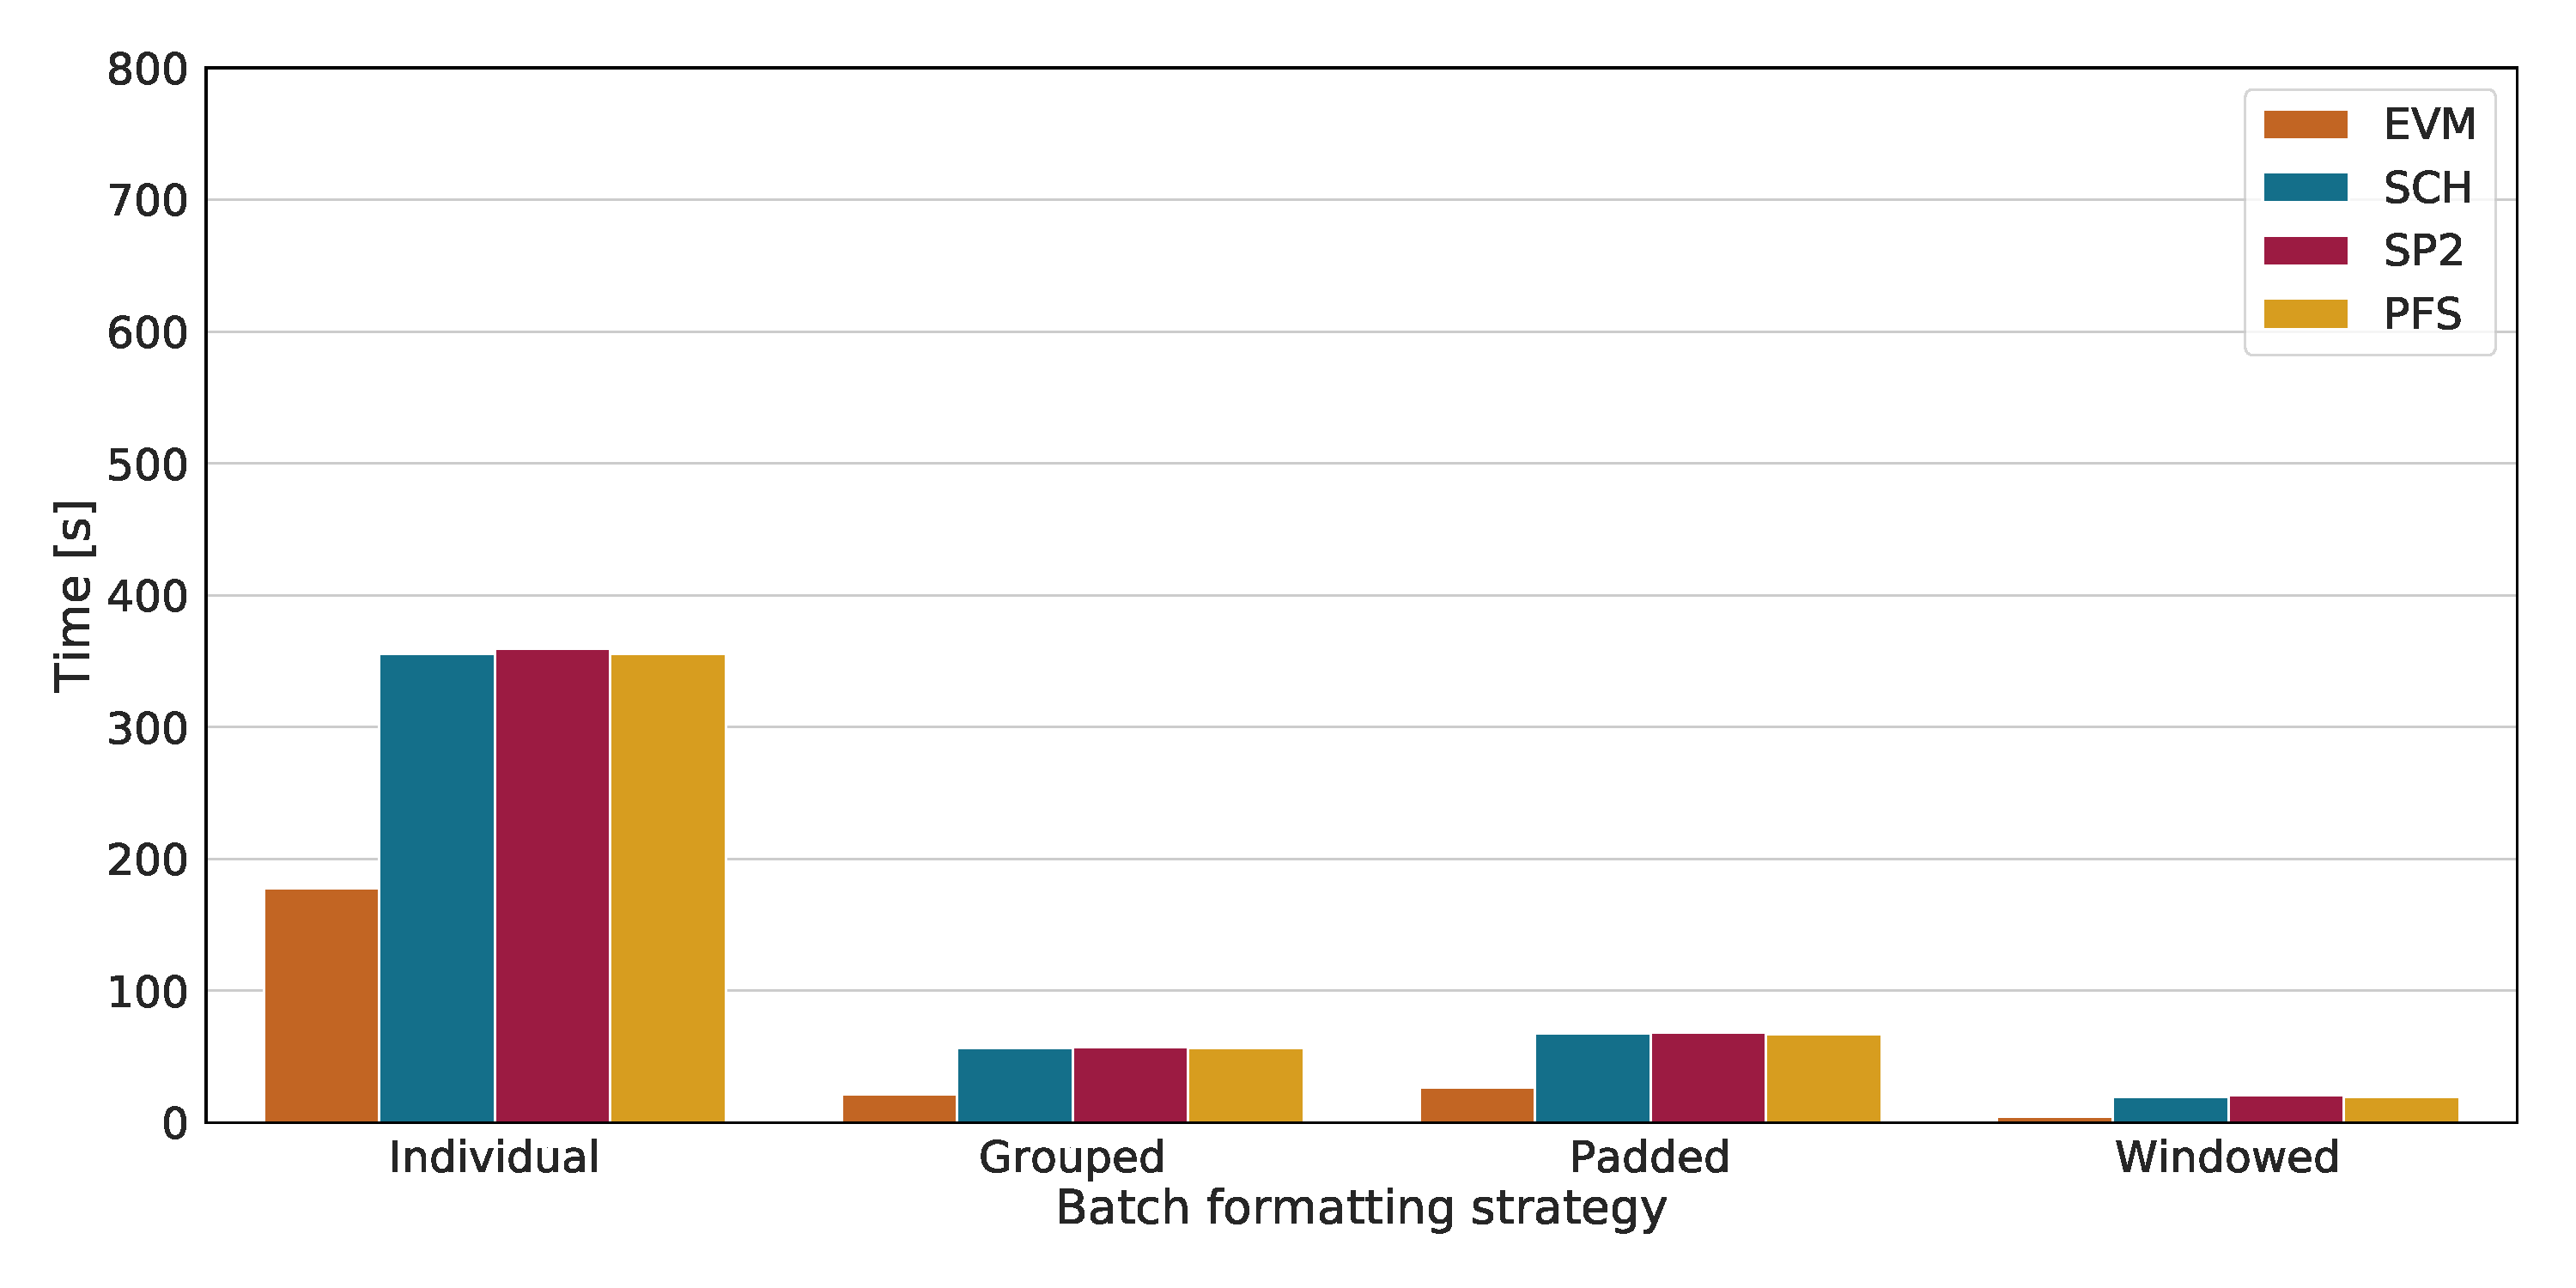
\includegraphics[width=\textwidth]{gfx/bpic2015_5/train_timings.pdf}
    \caption{Training times measured on BPIC15-5}
    \label{fig:BPIC15-5-training-timings}
\end{figure}

\paragraph{Training times on BPIC11}
\autoref{fig:BPIC11-training-timings} shows the training times measured on BPIC11.
On this plot, it is visible that the EVM model takes approximately half the training time of the other models.
As before, the other models require about the same time for an epoch for the same batching strategy.
The individual strategy causes the longest epochs, shortened a little by the grouping strategy.
The padding strategy incurs a big drop in training times, and the windowing strategy is the fastest, again.

\begin{figure}[!htb]
    \centering
    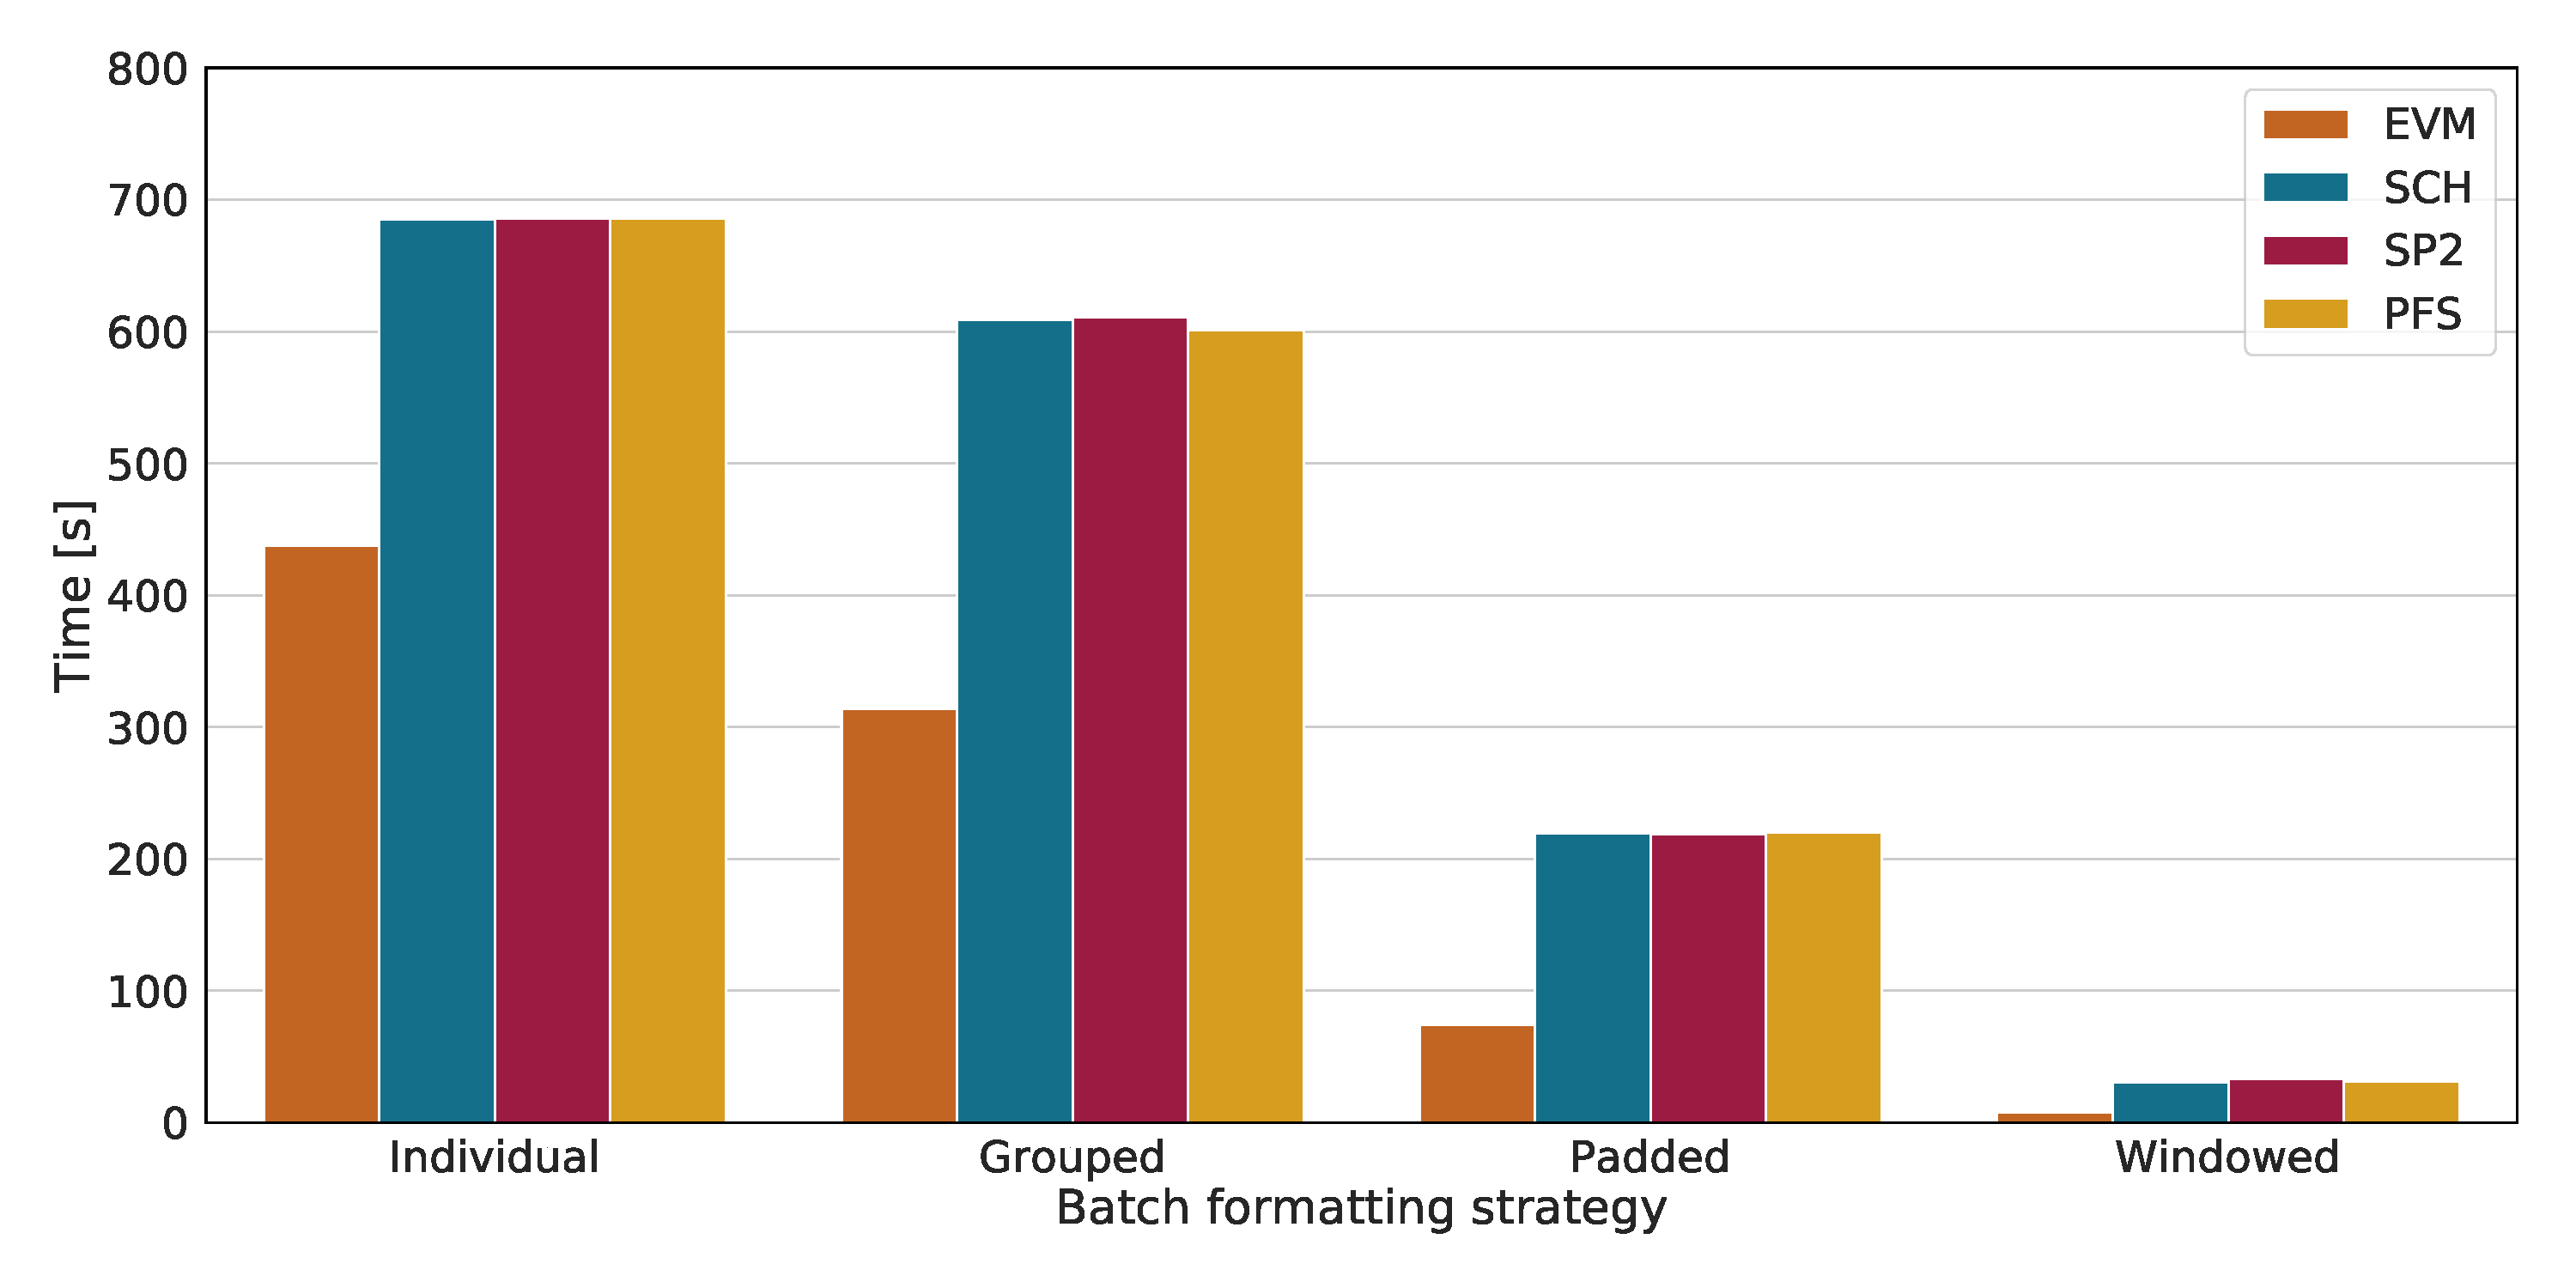
\includegraphics[width=\textwidth]{gfx/bpic2011/train_timings.pdf}
    \caption{Training times measured on BPIC11}
    \label{fig:BPIC11-training-timings}
\end{figure}

\paragraph{Verdict on training times}
Across all datasets, we gathered the following observations.
The individual strategy leads to the longest times overall.
This is not surprising, as \autoref{tab:dataset-characteristics} reveals that this strategy leads to hundreds of weight adjustments per epoch.

The grouping strategy leads to significant reductions in training times, depending on how diverse the trace lengths are. \autoref{tab:dataset-characteristics} explains why the reduction is not as prominent with BPIC11: It exhibits up to 1814 different lengths, while the other datasets only exhibit $5\%$ to $10\%$ of this number.

With the padding strategy, it is possible to overcome the limitations imposed by trace lengths and construct batches out of any number of traces. This makes it easier to optimize the batch size, which can lead to faster training times.

Finally, the windowing strategy is the fastest.
It produces a constant number of timesteps and allows for arbitrary batch sizes.
The low number of timesteps additionally reduces the amount of calculation that needs to be done.
\FloatBarrier

\section{Stability}\label{sec:eval:stability}
As we stressed in the introduction, the stability of a prediction model along the progress of a case can strongly impact the level of trust that users put into the model~\cite{metzger2015}.

In this section we show the stability plots produced on each log, one for each batching strategy.
We will show the stability per log, and finish with a verdict.
For space reasons, we will only present the most informative graph per log in this section, and enclose the others in \autoref{appendix:evaluation-measurements} for space reasons.

Each figure for a batching strategy and a dataset contains four curves, one for each model.
The curves show the model accuracy along the progression of all traces inside the validation set in steps of $5\%$.
The stability on the HelpDesk log was calculated in steps of $10\%$, as most cases in it are only 13 steps long.
The following paragraphs explains these curves in further detail.

\paragraph{Stability on HelpDesk}
On the HelpDesk log, it shows again that the batching strategies have a strong impact on the accuracy in different stages.

\autoref{fig:helpdesk-individual-stability} shows the stability of each model with the individual strategy.
The four curves start around $0.8$, and then stay at that level until $60\%$ progress.
The EVM model becomes less and less acurrate from the beginning.
At the $60\%$ mark, all curves show a small correction, before going up toward an accuracy of $1$ at the end.

\autoref{fig:helpdesk-grouped-stability}, \autoref{fig:helpdesk-padded-stability}, and \autoref{fig:helpdesk-windowed-stability} show the stability on the other strategies.
With the grouping strategy, the curves are very similar, with the expection of the EVM curve.
The EVM accuracy curve starts at around $0.05$, and goes toward $1$ at the end of the trace.

The padding strategy makes all four models become very unstable.
After the three SCH, SP2 and PFS curves start around $0.8$, the curves see degradations and fluctuation around the $50\%$ mark, with the PFS model completely failing at $0$ accuracy at the end.
The EVM model starts at an accuracy of $0$ and rises to $1$ at the end of all traces.

The windowing strategy makes the curves become very irrate.
All curves start at 0 accuracy, and stay below $0.5$ accuracy until $60\%$ progress.
At this point, the curves shoot up above $0.8$, and finish at an accuracy of $1$.

\begin{figure}[!htb]
    \centering
    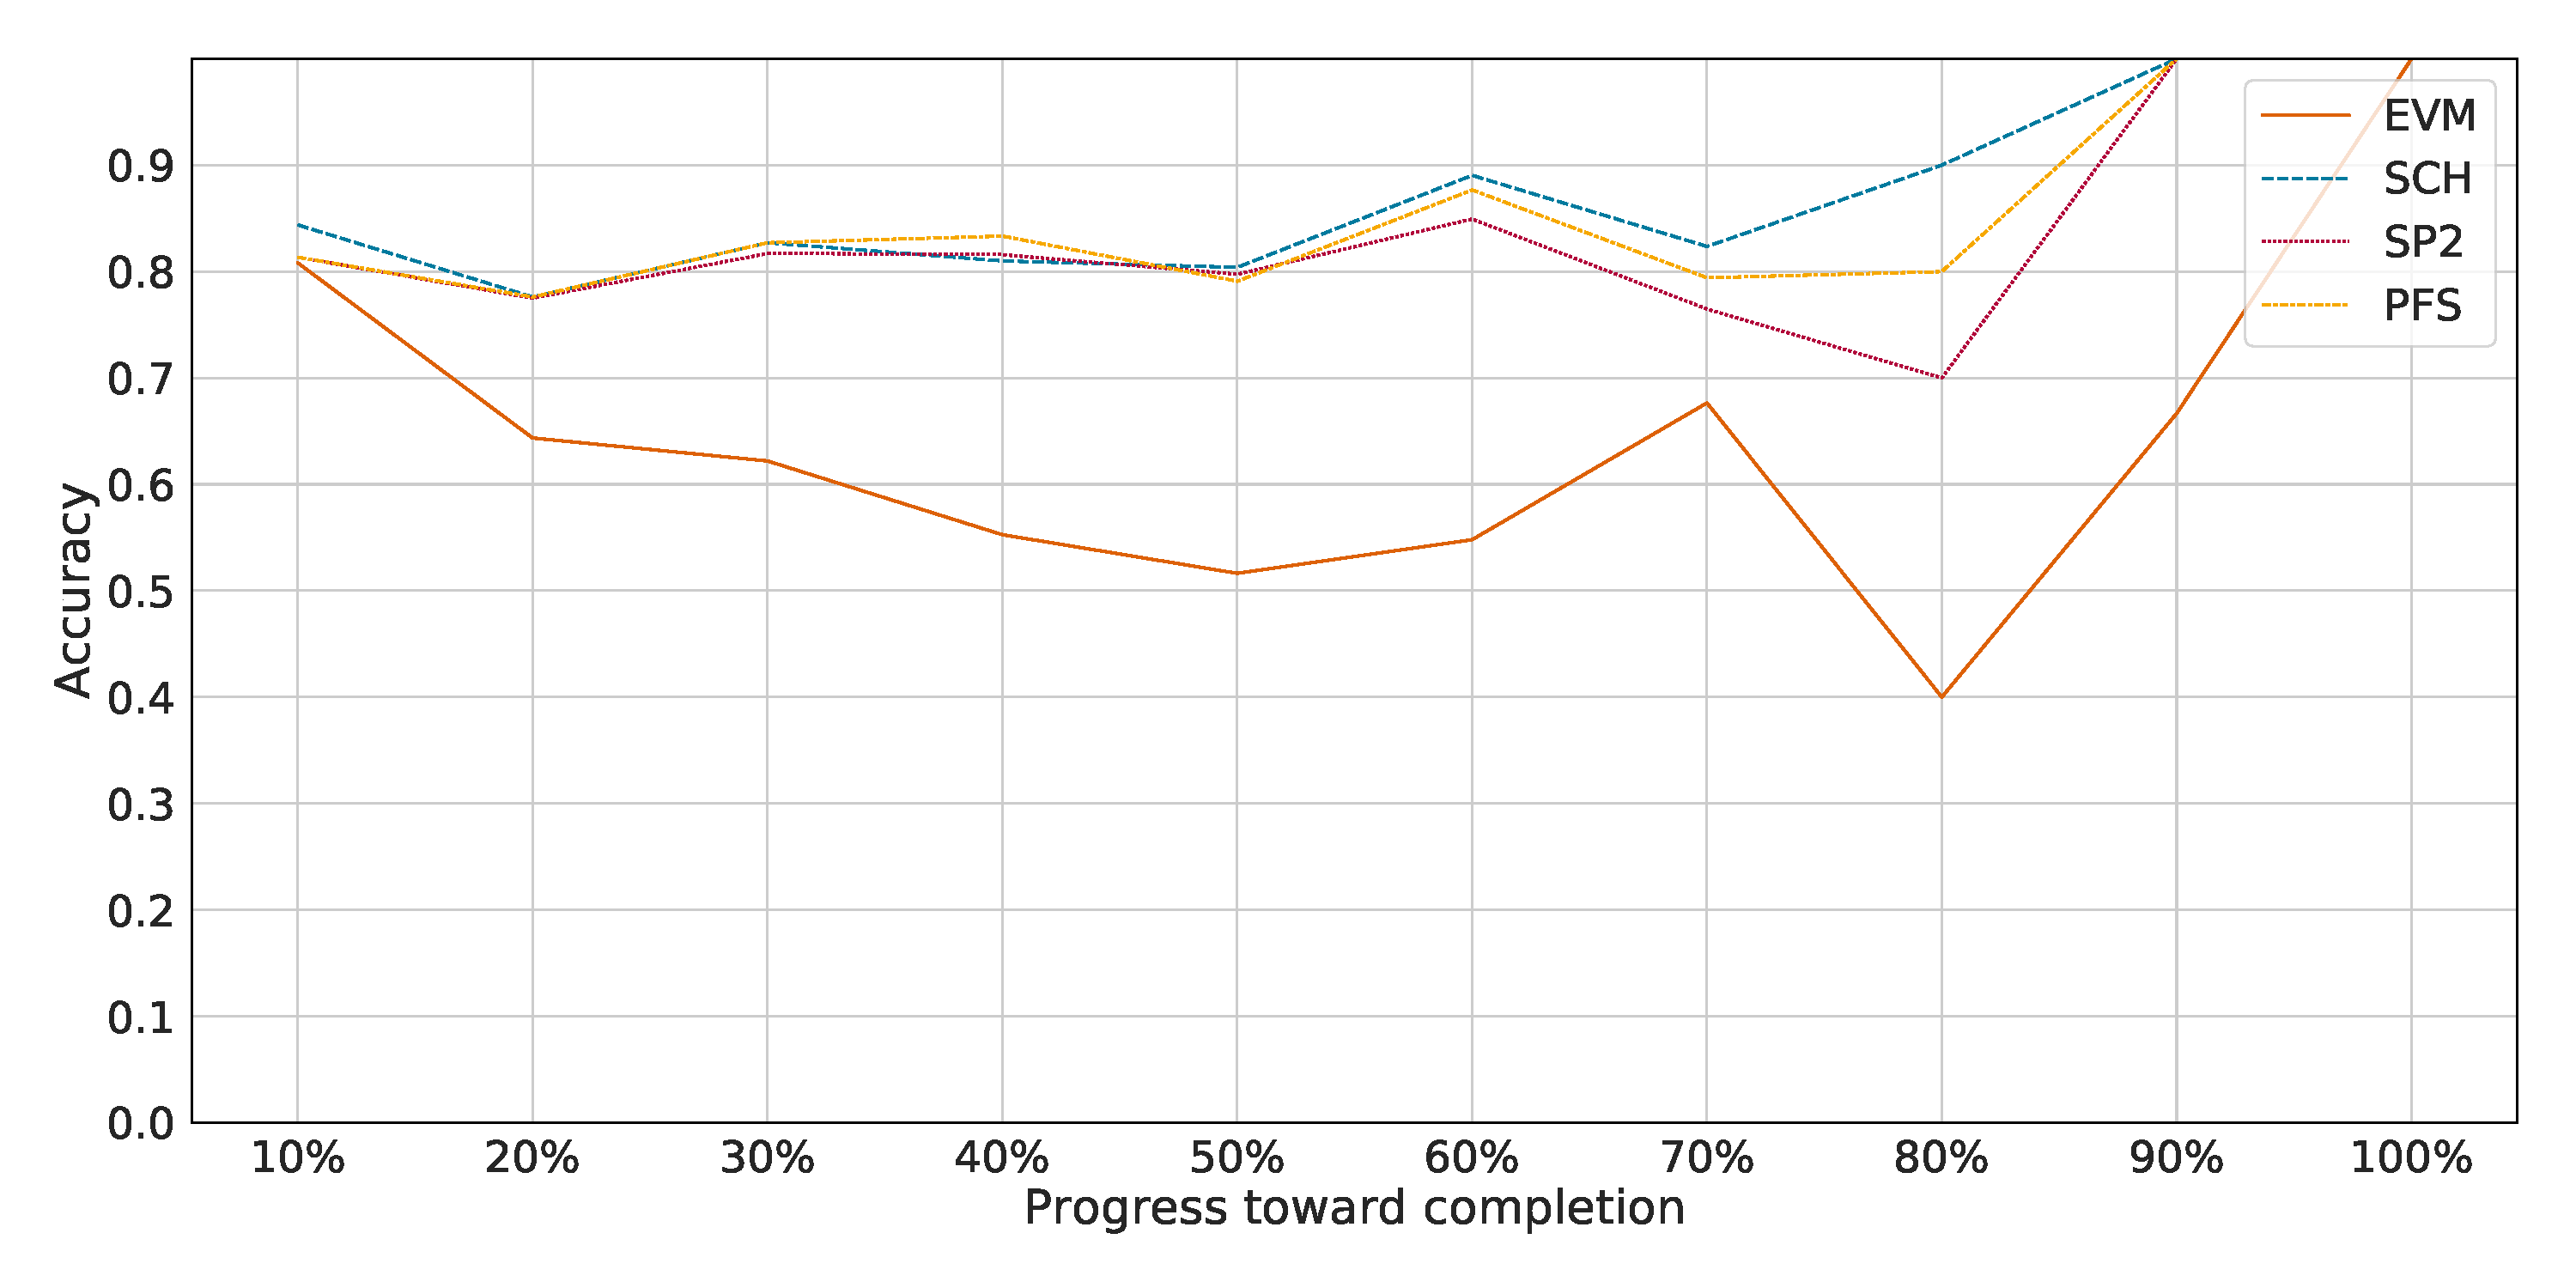
\includegraphics[width=\textwidth]{gfx/helpdesk/individual_stability.pdf}
    \caption{Model stability, individual strategy, HelpDesk}
    \label{fig:helpdesk-individual-stability}
\end{figure}

\paragraph{Stability on BPIC12}
\autoref{fig:bpic12-individual-stability} shows the stability of each model with the individual strategy on BPIC12.
The four curves start around $0.8$, and immediately drop by $0.2$.
The EVM curve does not recover from the drop, constantly stays around $0.4$, and finishes around $0.1$.
The other three curves rise back up to $0.9$ at $35\%$ progress.
Then, all three slowly sink toward $0.7$ at $85\%$, and rise up sharply toward $1$ at the end.

\autoref{fig:bpic12-grouped-stability} shows the stability for the grouping strategy.
The trajectories of all four curves are exactly as described for the individual strategy.
A small, but notable difference is that the curves of the SCH, SP2 and PFS models are much closer together, and indicate nearly the same values.

In \autoref{fig:bpic12-padded-stability}, the stability for the padding strategy is shown.
The curve trajectories are again very similar to the two aformentioned stability plots, but the overall accuracies are lower.
The EVM model now starts at $0$ accuracy, shortly reaches $0.3$ around $25\%$ and then tapers off back into $0$ accuracy at the end.
The other three curves show a stronger depression around the $75\%$ mark, dropping down to an accuracy of $0.5$, before recovering to $1$ at the end.

Finally, the stability plot of the windowing strategy in \autoref{fig:bpic12-windowed-stability} reveals completely new curve trajectories.
The EVM curve starts again at $0$, slowly rises to $0.3$, and then edges back down to $0$ in the end.
The SP2 curve starts at $0.8$, drops by $0.1$, and recovers back to $0.9$ until $50\%$ progress.
At this point, there is a sharp decline to $0.7$.
The curve recovers just as sharply, and slowly degrades to $0.6$, and shoots up to $1$ in the end.
The SCH and PFS curves show a similar trajectory as the SP2 curve, albeit less accurate by around $0.150$.

\begin{figure}[!htb]
    \centering
    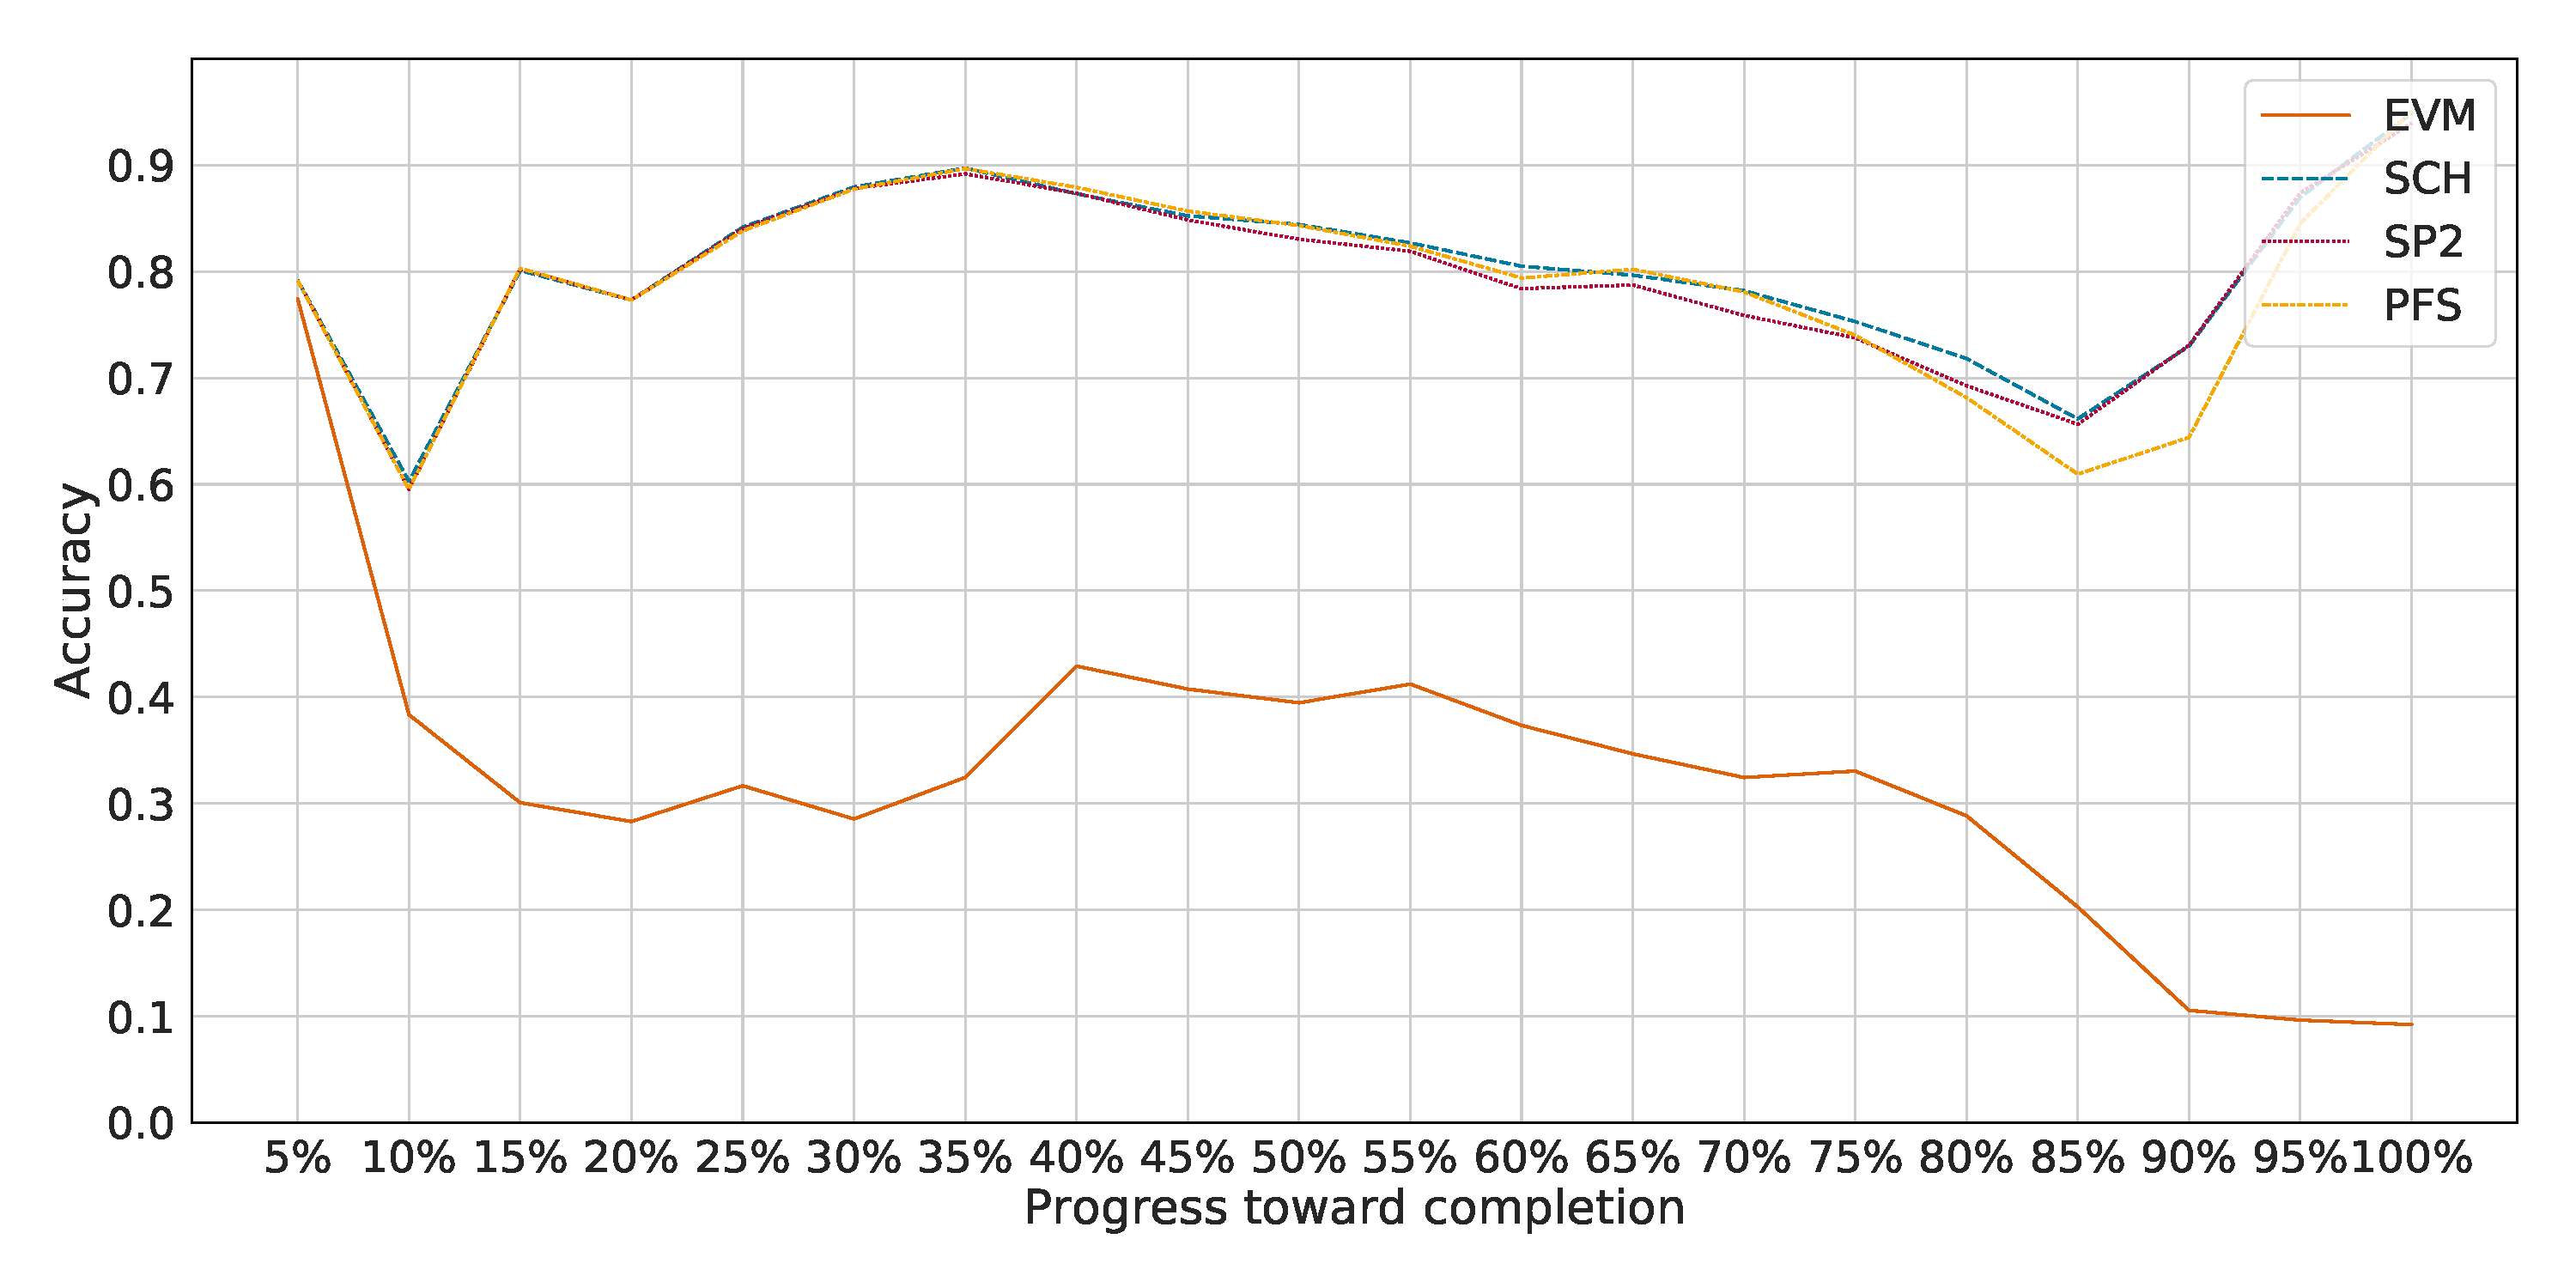
\includegraphics[width=\textwidth]{gfx/bpic2012/individual_stability.pdf}
    \caption{Model stability, individual strategy, BPIC12}
    \label{fig:bpic12-individual-stability}
\end{figure}

\paragraph{Stability on BPIC15}
The BPIC15 log with its five datasets is discussed in this paragraph.
The figures \autoref{fig:bpic15-5-individual-stability} and \autoref{fig:bpic15-5-grouped-stability} show the stabilities for the individual and grouping strategies on BPIC15-5.
In the appendix, \autoref{fig:bpic15-1-individual-stability} to \autoref{fig:bpic15-5-windowed-stability} illustrate the remaining curves for the remainder of the log.
The curves across BPIC15-1 to BPIC15-5 for a specific strategy are very similar, which is why we give a general description of the observations for each strategy in the following.

In the stability plot of the individual strategy in \autoref{fig:bpic15-5-individual-stability}, the EVM curve shows a very low accuracy.
Similar to the two logs before, the curve starts off with a steep decline from $0.5$ to $0.1$, and then stays around this accuracy. At the end, the curve shoots up to $0.35$.
The SCH, SP2 and PFS curves all start at $0.7$, and slowly sink down to around $0.5$ at $80\%$.
Then, all three curves see a $0.2$ increase, with the SP2 curve ending at $0.75$.
The SCH curve ends at $0.7$, and the PFS curve at $0.6$.

The stability plot for the grouping strategy in \autoref{fig:bpic15-5-grouped-stability} shows very similar curve trajectories.
In contrast to the individual strategy, the SCH, SP2 and PFS curves are a lot closer together, and the PFS model does not see as sharp a drop.
This is a theme that is visible on the other BPIC15 datasets, too.

The stability plots for the padding strategy show steadily declining curves for SCH, SP2 and PFS models from $0.7$ at the beginning towards an accuracy of $0.4$ around $90\%$.
Then, the curves jump up by $0.2$ to $0.3$ to finish around $0.7$.
The EVM curve barely surfaces above $0$.
For BPIC15-1 and BPIC15-4, the SCH curve also dips down after the start.
On BPIC15-1, the PFS curve also dips down, leaving the SP2 curve alone on the steadily declining trajectory previously described.

The plots for the windowing strategy show a common picture.
The EVM curves are stuck at 0.
The SCH and PFS curves start around $0.6$, and descend toward $0.3$, spiking up toward $0.5$ at the end.
The SP2 curve hovers above, starting around $0.7$, and linearly descends to $0.5$ until $90\%$.
Then, it also jumps up by $0.3$ at the end of the plot.

\begin{figure}[!htb]
    \centering
    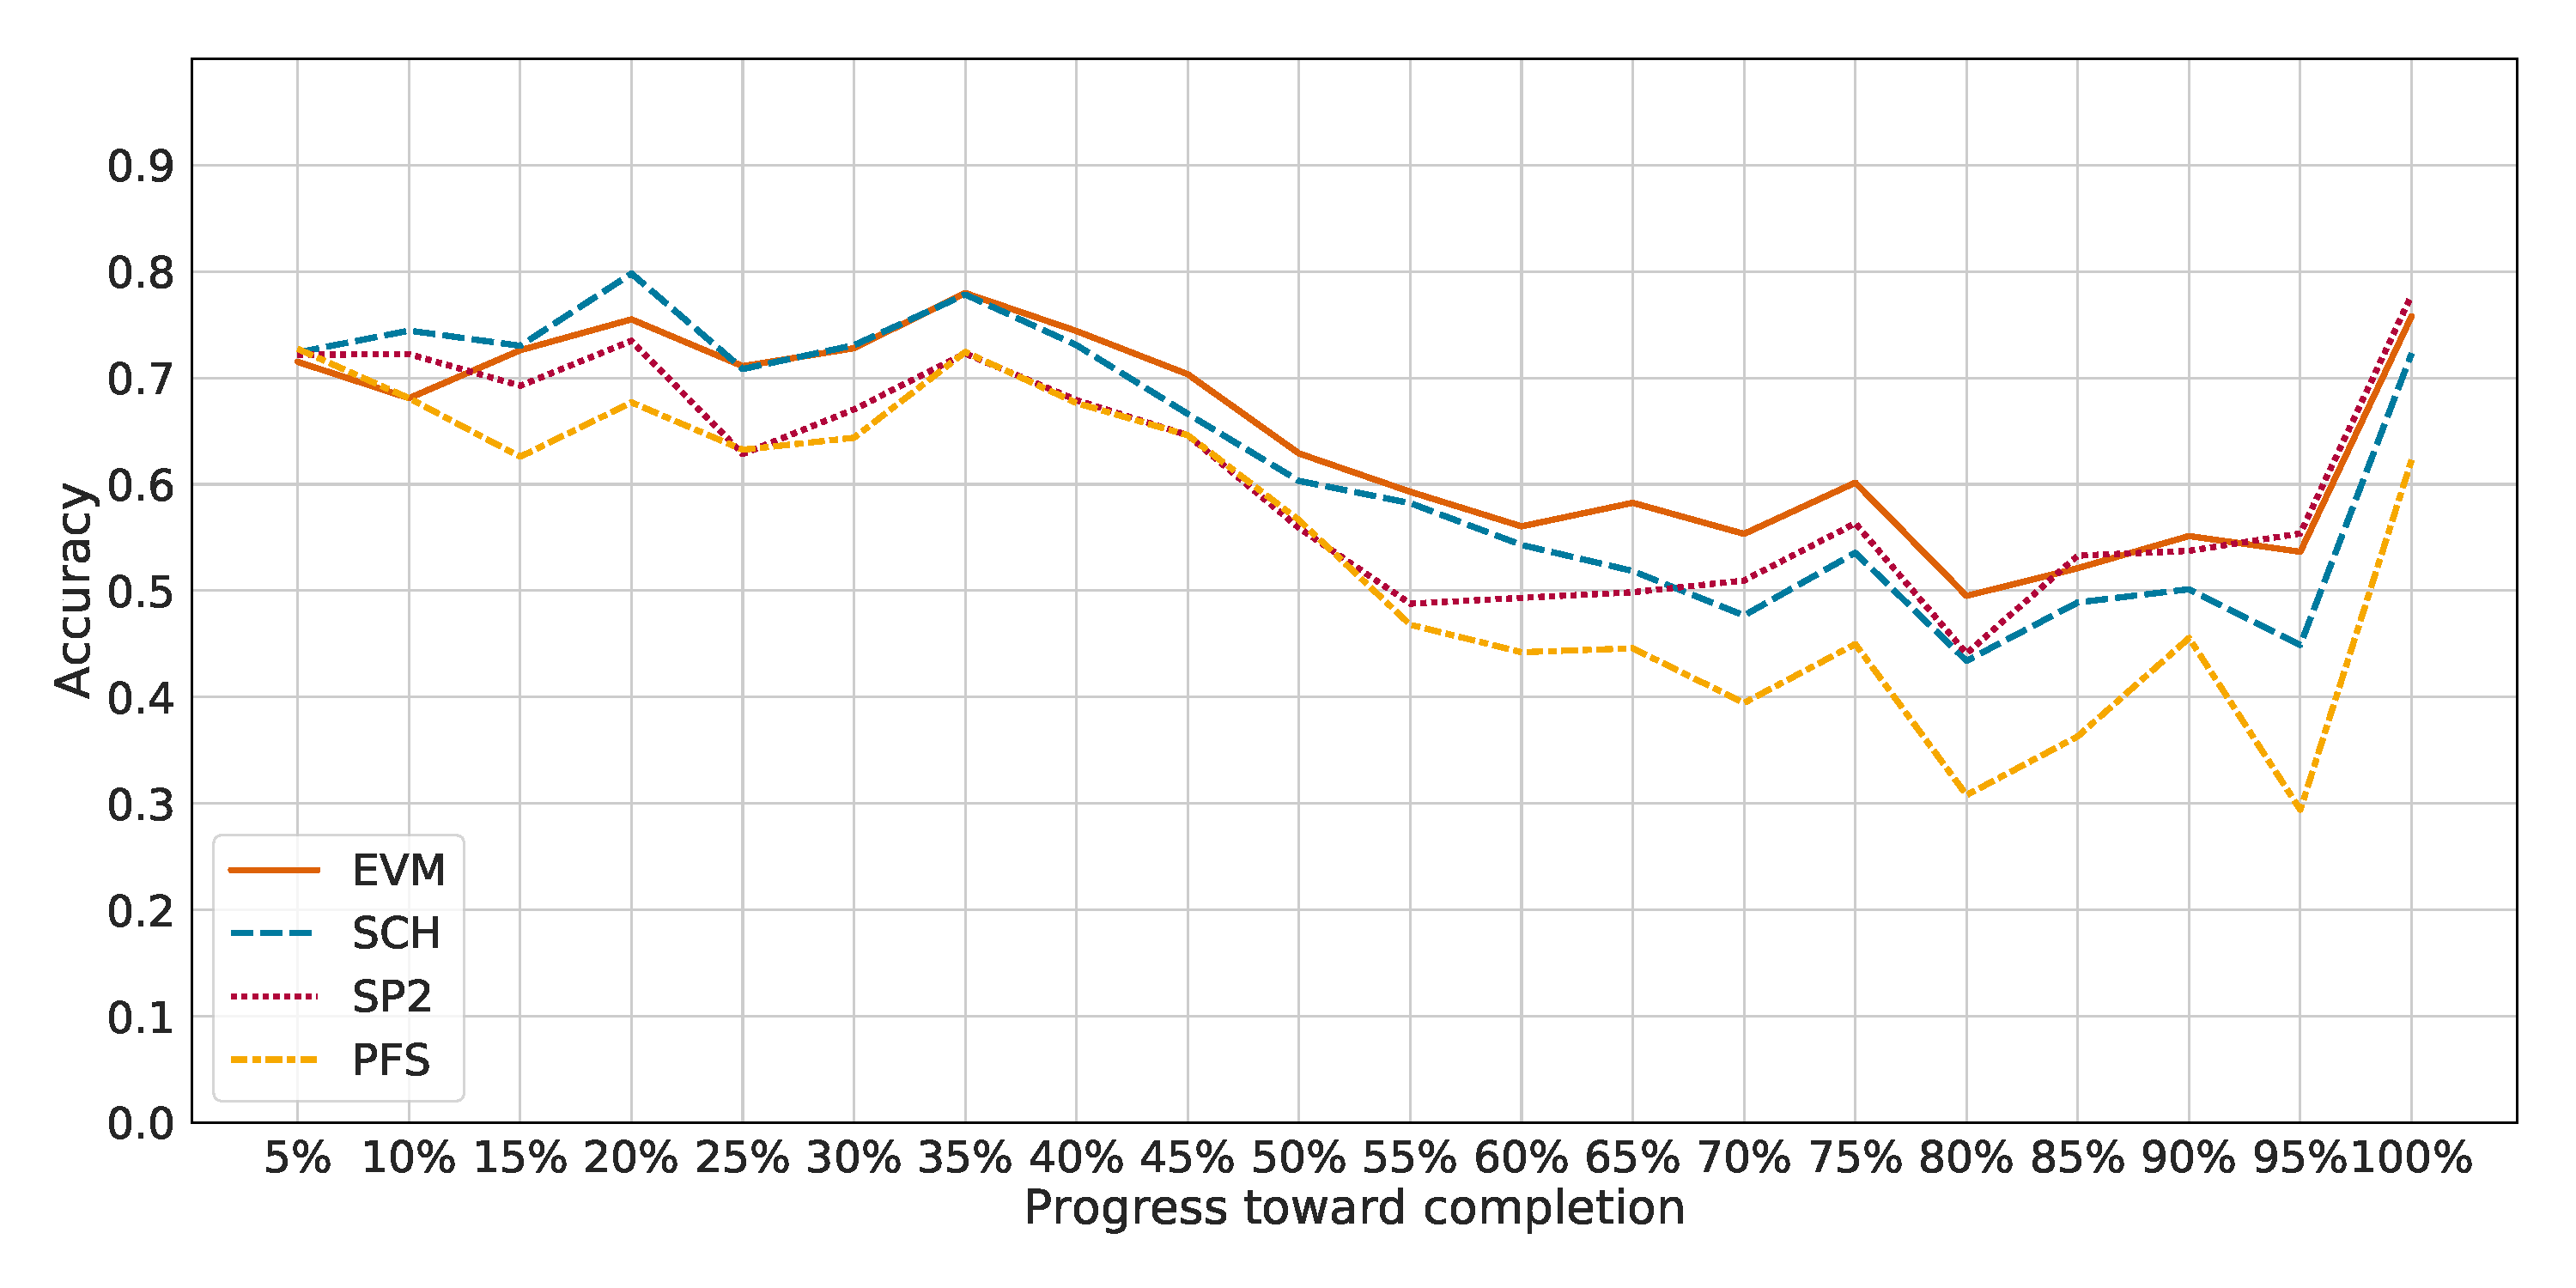
\includegraphics[width=\textwidth]{gfx/bpic2015_5/individual_stability.pdf}
    \caption{Model stability, individual strategy, BPIC15-5}
    \label{fig:bpic15-5-individual-stability}
\end{figure}
\begin{figure}[!htb]
    \centering
    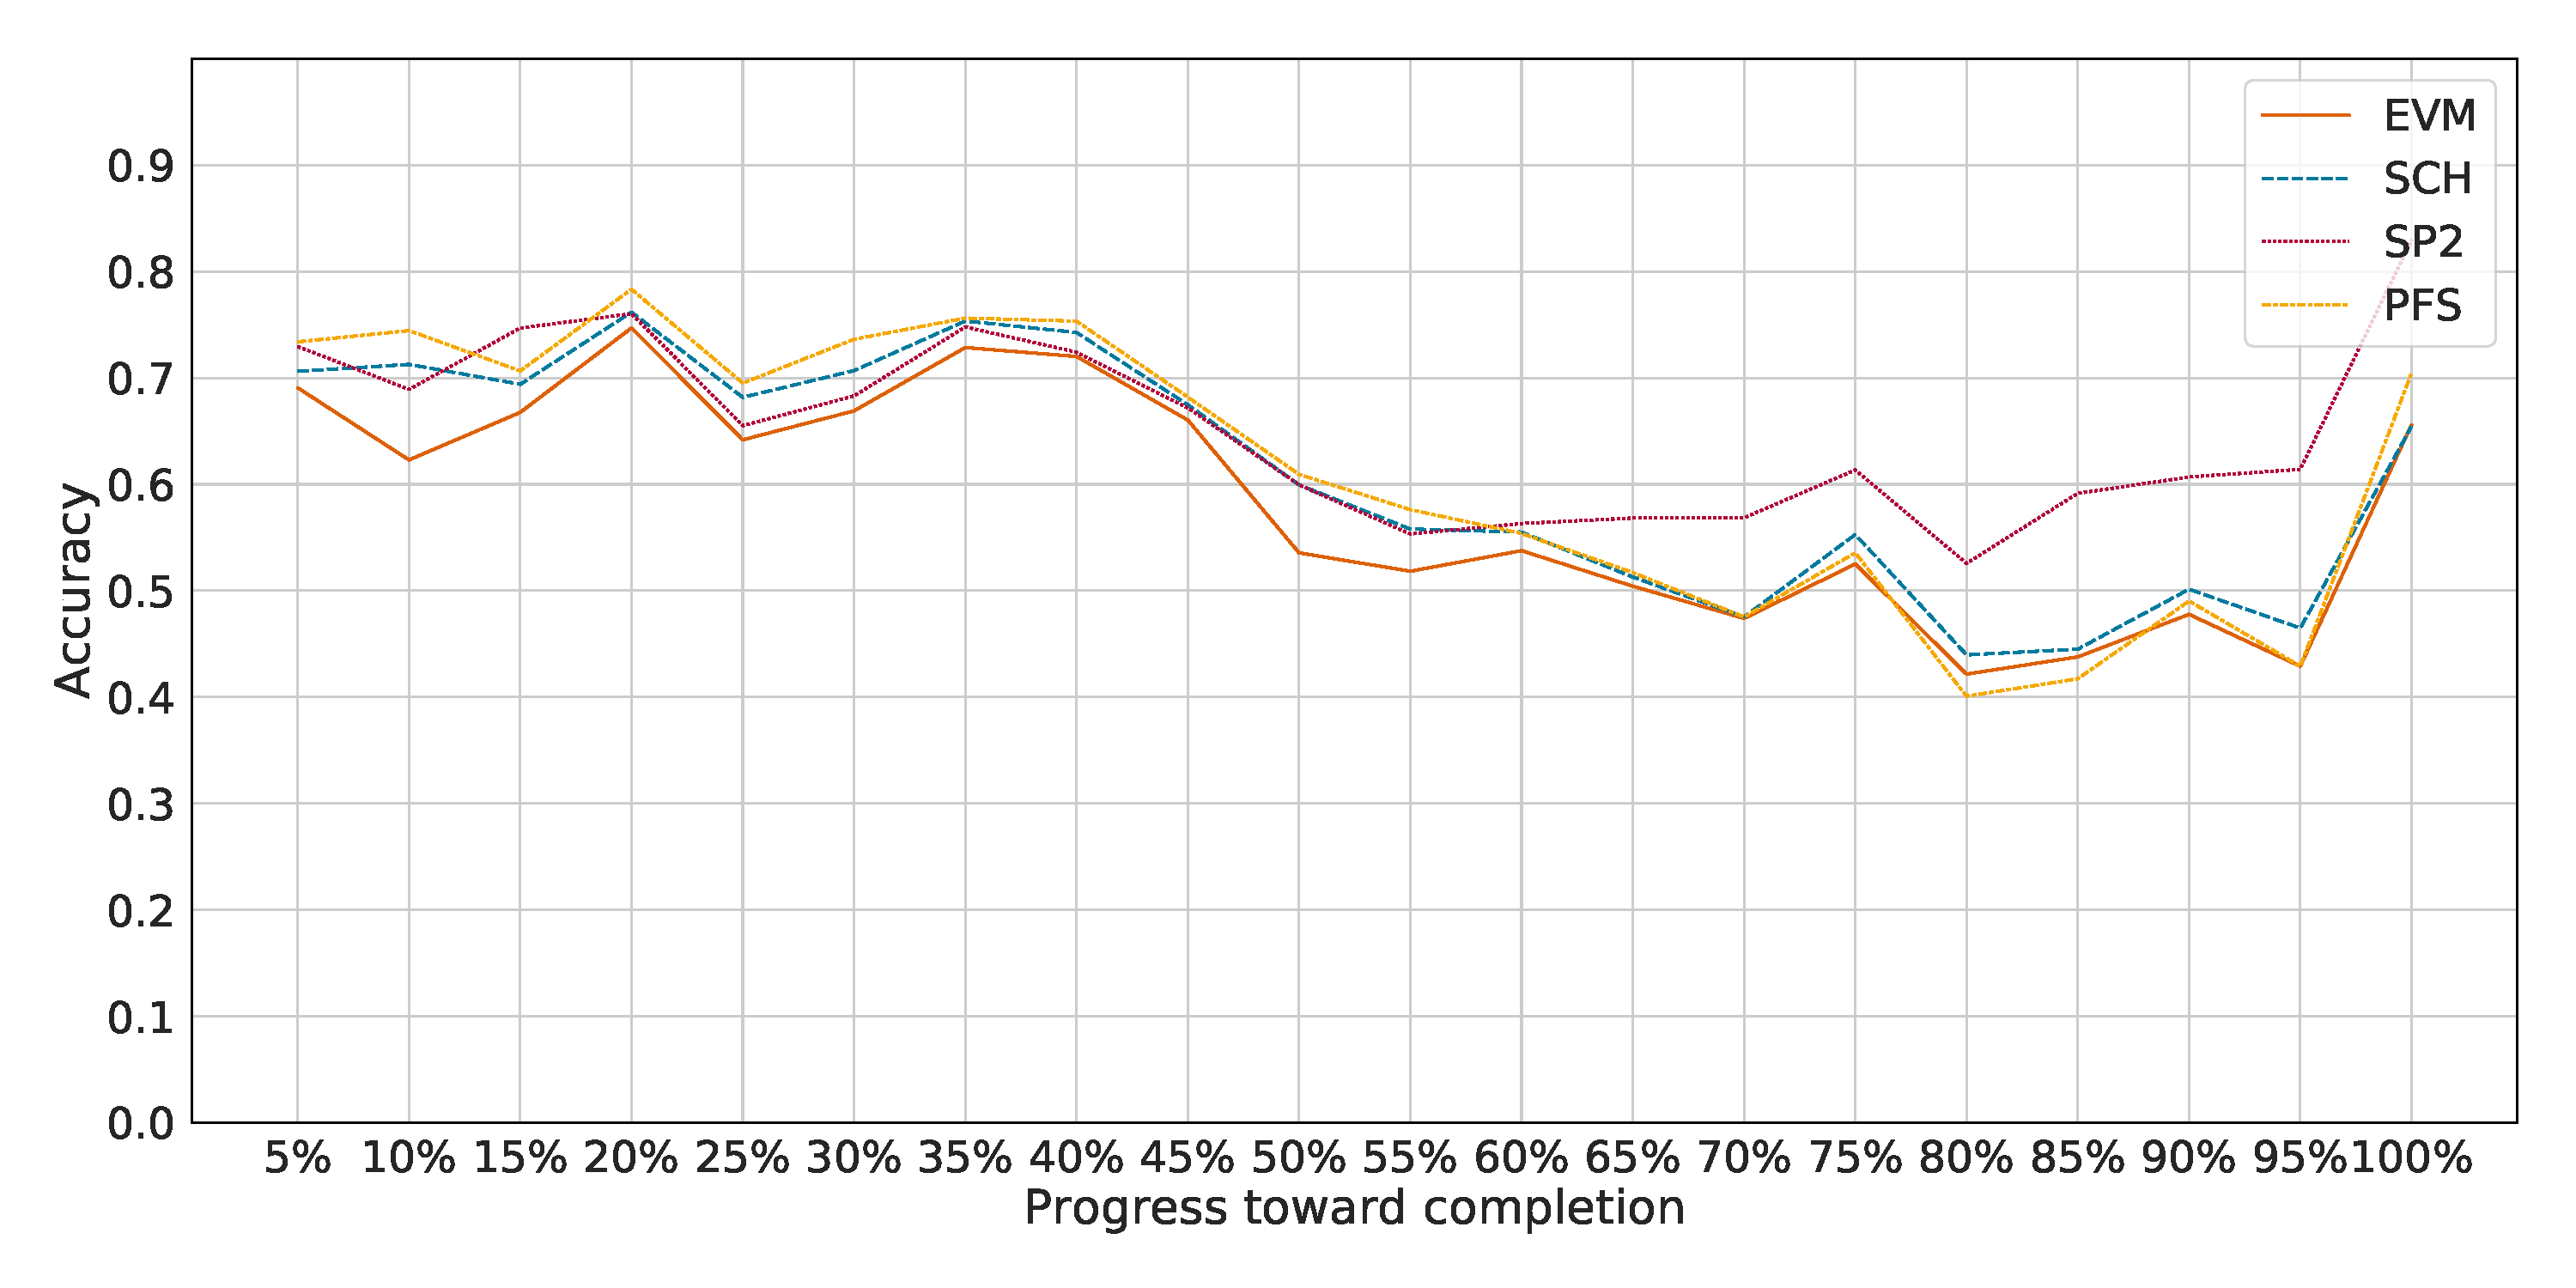
\includegraphics[width=\textwidth]{gfx/bpic2015_5/grouped_stability.pdf}
    \caption{Model stability, grouping strategy, BPIC15-5}
    \label{fig:bpic15-5-grouped-stability}
\end{figure}

\paragraph{Stability on BPIC11}

\paragraph{Verdict on stability}
What was presented in \autoref{sec:eval:accuracy} as a single digit --- connection to process complexitiy in different stages

% TODO harmonization of curves
% TODO spike at the end
% TODO EVM model is bullshit

The individual strategy not only takes the most time, but it also leads to strong differences between the SCH, SP2, and PFS models. A good example is the difference between \autoref{fig:bpic15-3-individual-stability} and \autoref{fig:bpic15-3-grouped-stability}. In the latter figure, the SCH, SP2 and PFS curves are a lot closer to each other.

The grouping strategy increases the sample count per batch, and this seems to have a harmonizing effect on the results as evidenced by the corresponding figures of all datasets. This harmonizing effect is manifested in the reduction of the standard deviation of the best accuracies of the SCH, SP2 and PFS models in \autoref{fig:grouping-accuracy-harmonization}.

\begin{figure}
    \centering
    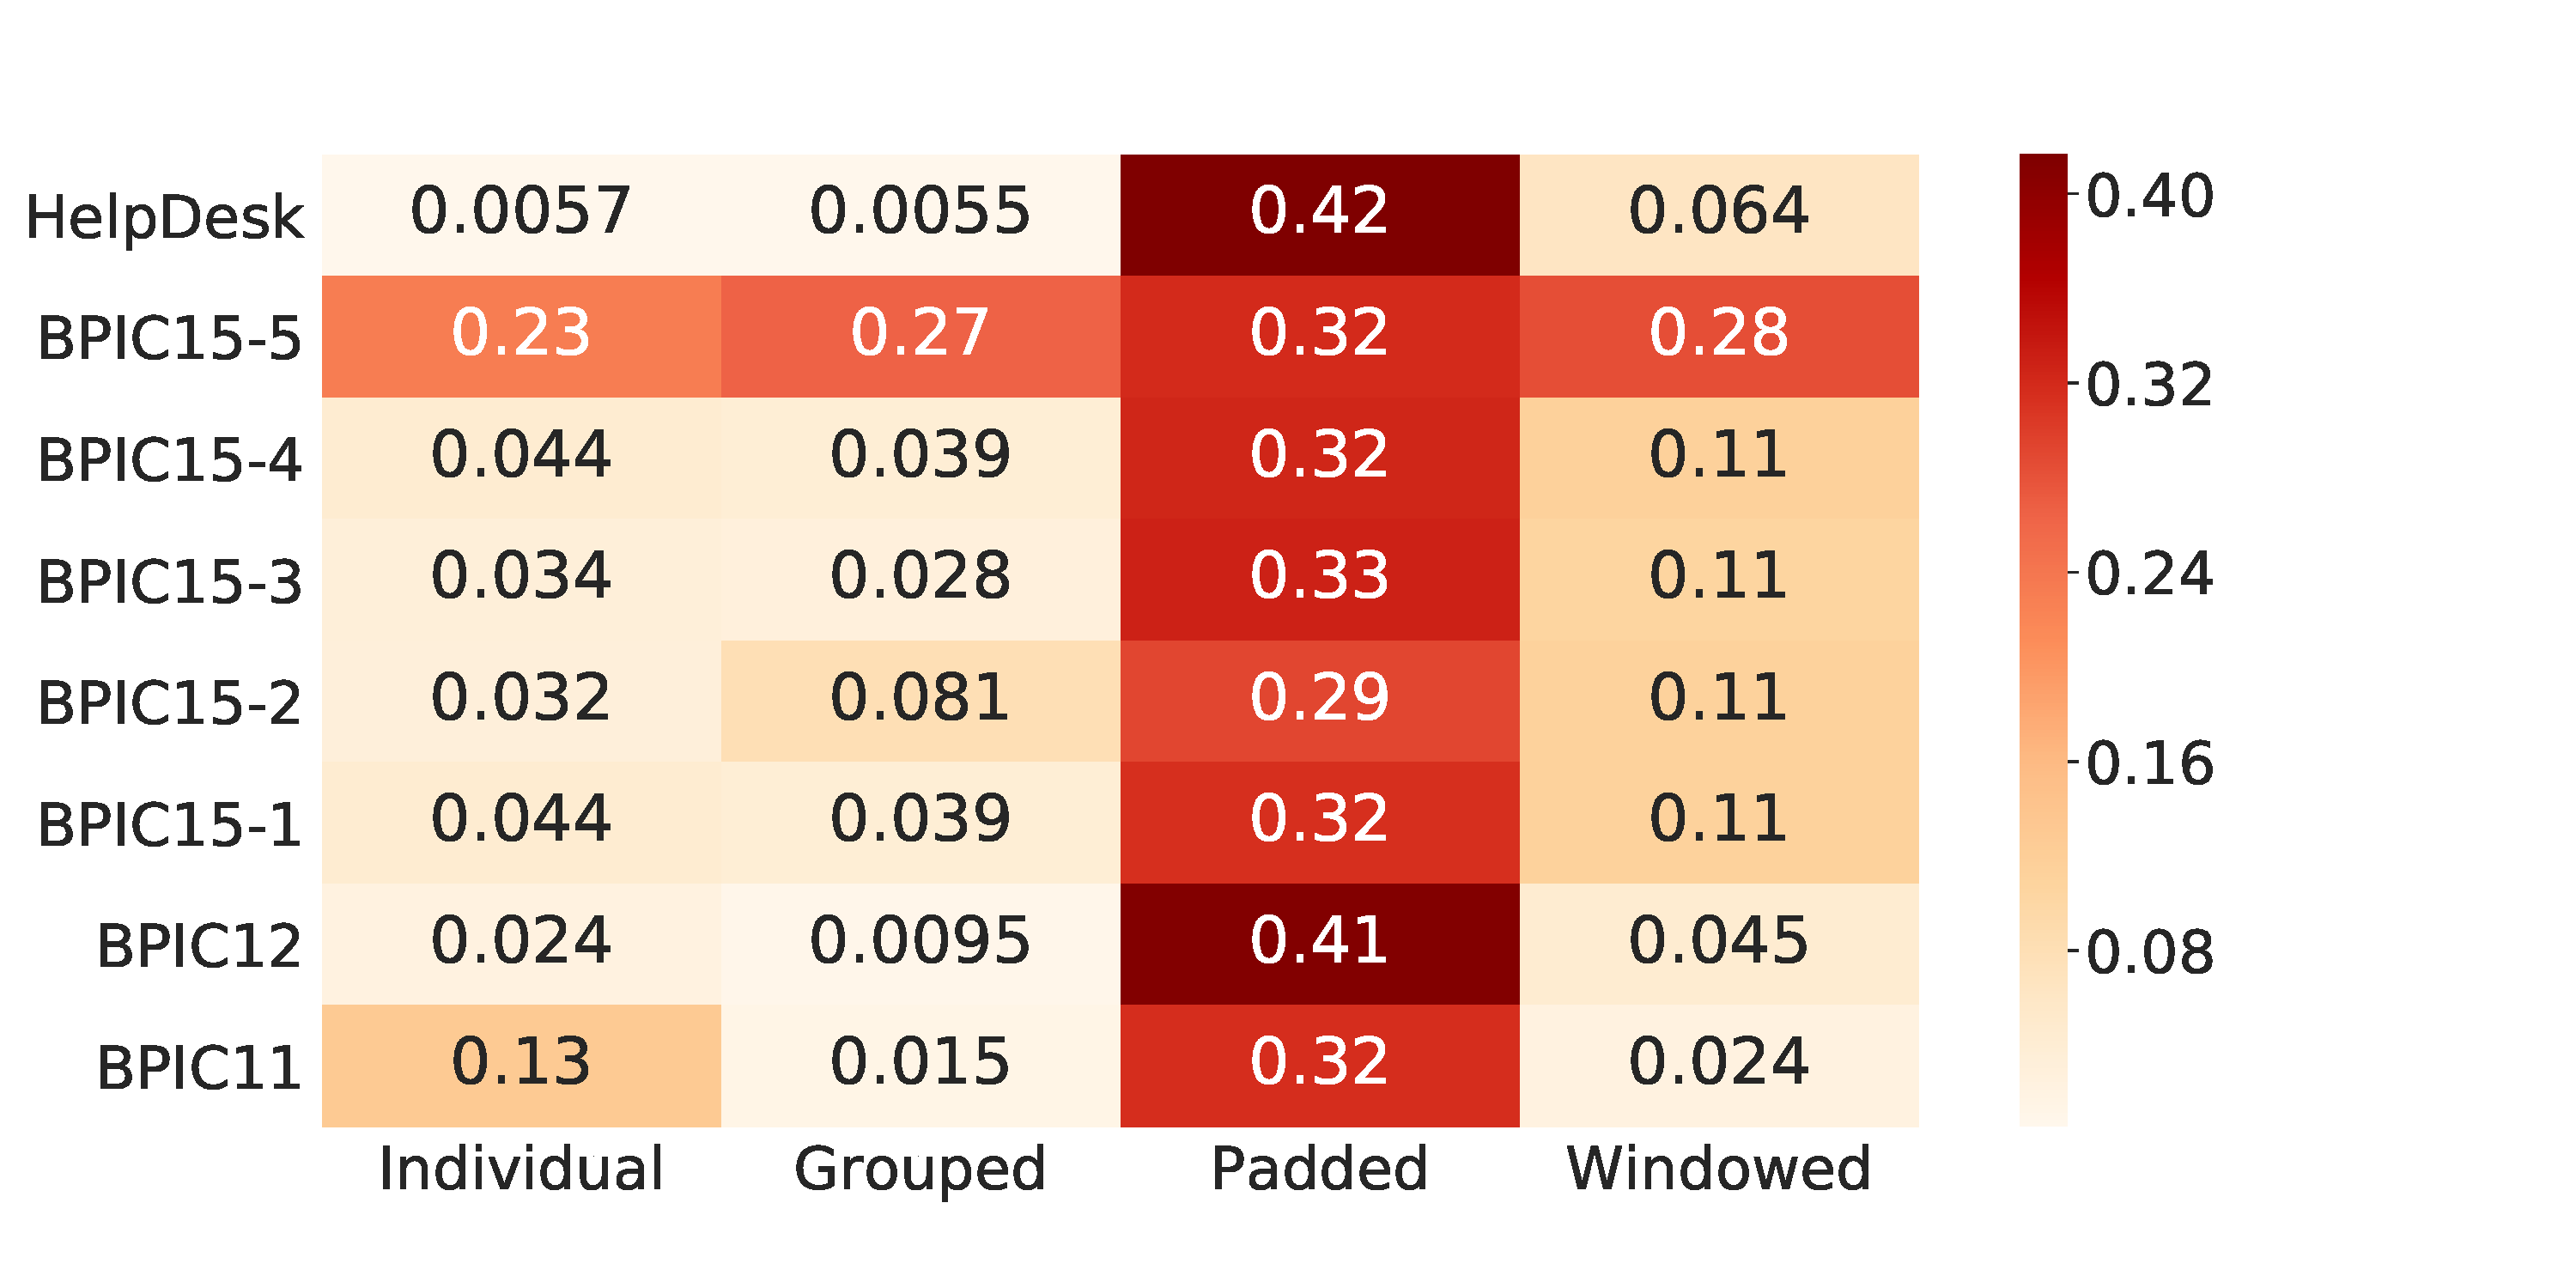
\includegraphics[width=\textwidth]{gfx/grouping-accuracy-harmonization.pdf}
    \caption[Batching strategy harmonizes top accuracies]{The grouping strategy often reduces the standard deviation between the highest accuracies of SCH, SP2 and PFS models}
    \label{fig:grouping-accuracy-harmonization}
\end{figure}

The padding strategy yields results that are very similar to the grouping strategy - except on BPIC11 and HelpDesk. In the former case, the training data had to be trimmed because the padded traces had required too much memory. In the latter case, the batch size seems to have had a profound effect on accuracy.

Klinkmüller et al. state that the windowing strategy leads to unstable results~\cite{klinkmuller2018reliablemonitoring}. While this statement seems to be especially true for the longer processes in BPIC11 and BPIC15, the windowing strategy seems to have less of an impact with shorter processes as evidenced with BPIC12. There, all models show a dip towards the end of the trace.\\

Generally, models were expected to become more accurate as the trace neared its end. However, this did not turn out to be the case. Instead, the accuracy was high when variability in the respective stage of the process was low. For example, processes in BPIC11 always begin similarly, as patients need to be onboarded~\cite{bose2011analysis}. The connection of accuracy and variability could be a cause for the high accuracies at the beginning of the BPIC11 stability curves. The processes in BPIC12 always end either on approval or dismissal of the application, making the models very accurate in this stage~\cite{adriansyah2012mining}.

\section{Discussion}\label{sec:eval:discussion}
After presenting and explaining our findings, we summarize our learnings in this section and compare our findings to the papers mentioned in \autoref{sec:method:dataset-choice}.\\

First, we can to confirm Klinkmüller et al.~\cite{klinkmuller2018reliablemonitoring} and their suspicion that the windowing strategy does not work well for sequence prediction. While it may be a performant strategy to use for time-series prediction, it does not work very well for predicting the future of a single case.

Second, we find that the grouping strategy frequently delivers the best results in terms of speed and accuracy. We realized that it should be iterated upon to include a threshold which limits batches to a maximum size and splits the larger batches accordingly. As evidenced by the charts, the grouping strategy seems to perform better with a medium to highly complex processes from BPIC11 and BPIC15, while padding works better with the more straightforward process from BPIC12. In combination with the SP2 model, the grouping strategy contributed to most of the highest accuracies.

Third, we realize that Embeddings might not be useful on the currently available datasets as these might have not enough samples. The lacking performance of the EVM model and its barely converging loss indicate that this might be the case. All accuracy/loss curves from training are enclosed in \autoref{appendix:loss-curves}, and show that especially for the EVM model, the loss optimization does not work correctly.\\

We end the evaluation with a comparison of our best results with the initially mentioned publications based on BPIC12. While Evermann et al.~\cite{evermann2016} were able to obtain an accuracy of $0.768$, they did not focus on specific cases. Furthermore, Evermann et al. did not use Keras on top of Tensorflow but Tensorflow directly, which enabled him to make use of low-level functions directly. To the best of our knowledge, our implementation sufficiently approximates theirs, but this can be a reason for the low accuracy. Another very probable reason is their feature engineering~\cite{evermann2016}.

On BPIC12 and the HelpDesk log, Böhmer et al.~\cite{boehmer2018probability} attain an accuracy of $0.77$ with their statistical approach. While they argue that machine learning methods may perform better, they place great value on comprehensible reasoning information from the model.

Tax et al.~\cite{tax2017} reach a maximum accuracy of $0.76$ in their paper on BPIC12 and $0.71$ on the HelpDesk log.

Using the individual strategy, all SCH, SP2, and PFS score above $0.80$ on both datasets.
This surpasses all three aformentioned results.
The SCH model edges to the best accuracy of $0.853$, with the SP2 model close at $0.851$ on BPIC12.
On the HelpDesk dataset, the PFS and SCH models reach $0.862$ and $0.854$.
The fact that our accuracy surpasses that of Böhmer et al. supports their thesis of lower comprehensibility at higher accuracy.\\

In this evaluation we discussed the performances of the models on the individual datasets.
We determined that the grouping strategy delivers good results, but can still be optimized.
Furthermore, we noted that the complexity of the traces in the log has a large impact on stability.
Depending on the amount of variability in different stages of the process, model accuracy varies dramatically.
We could confirm that our models outperform recently published approaches, and describe how it can be improved in the next chapter.
We then conclude the thesis with a summary of the results.
